\documentclass{article}
\usepackage{amsmath,mathtools}
\usepackage[utf8]{inputenc}
\usepackage[ngerman]{babel}
\usepackage{acronym}
\usepackage{graphicx} 
\usepackage{epstopdf}
\usepackage{svg}
\usepackage{multirow}

%Hyperlinks package, links aus inhaltsverzeichnis
\usepackage[hidelinks]{hyperref}
\hypersetup{
    colorlinks=false, %set true if you want colored links
    linktoc=all
}
%Blattformatierung
\usepackage{geometry}
\geometry{a4paper, top=25mm, left=30mm, right=25mm, bottom=20mm}

\begin{document}
\tableofcontents

\newpage
\section{Spektren bei Konstant- und Nullsignal}
\begin{figure}[h!]
DFT-Spektren wurden über $n=7500$ Messwerte berechnet, Leistungsdichtespektren über $2*n=15000$ Autokorrelationswerte.
\centering
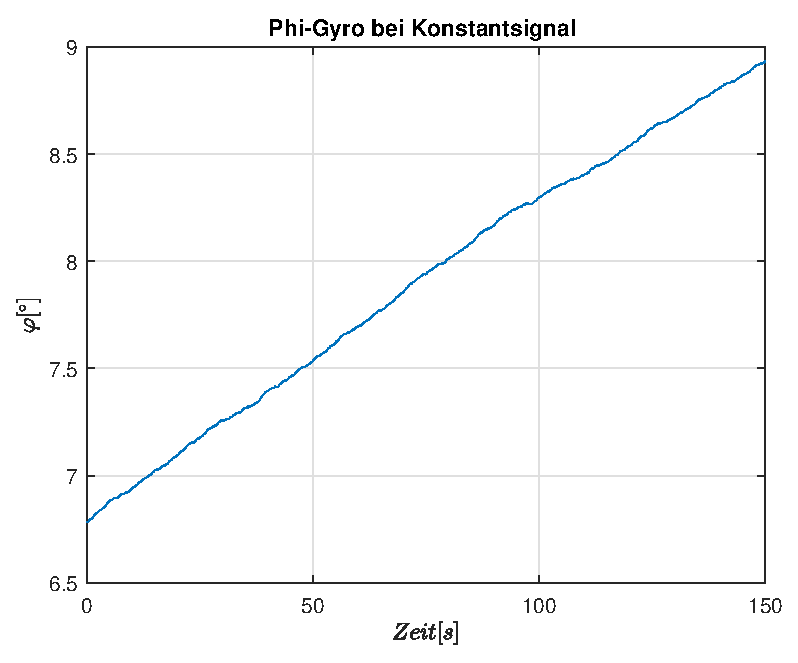
\includegraphics[width=0.5\linewidth]{img/phi_g_constsig}
\end{figure}
\begin{figure}[h!]
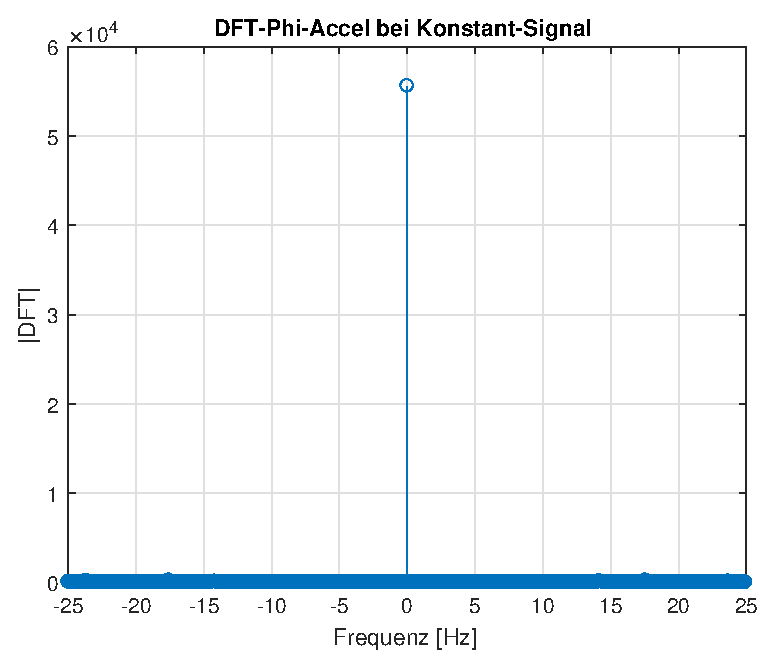
\includegraphics[width=0.5\linewidth]{img/dft_phi_a_constsig}
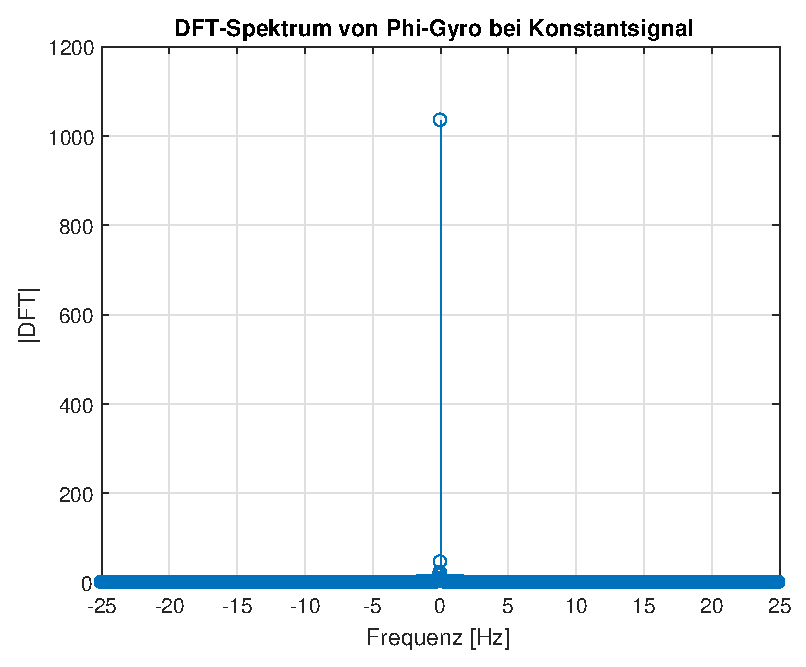
\includegraphics[width=0.5\linewidth]{img/dft_phi_g_constsig}
\end{figure}
\begin{figure}[h!]
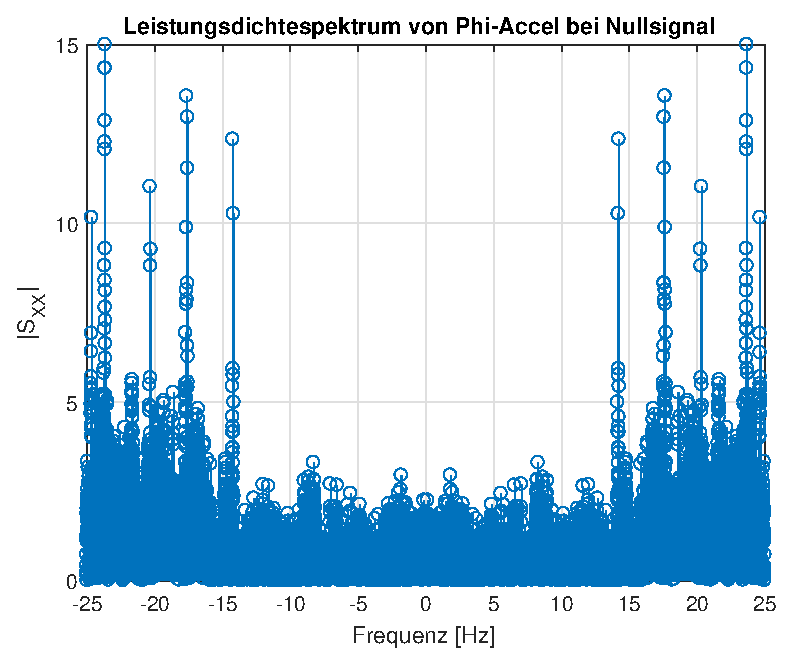
\includegraphics[width=0.5\linewidth]{img/lds_phi_a_zerosig}
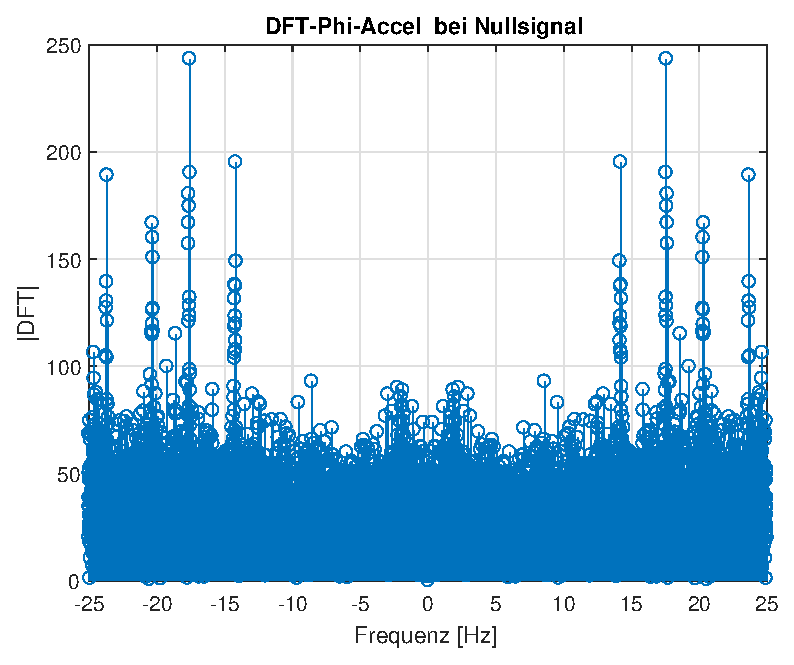
\includegraphics[width=0.5\linewidth]{img/dft_phi_a_zerosig}
\end{figure}

\newpage
\section{Spektren von $\varphi$ aus Winkelschätzung bei Sinusanregung}
\subsection{DFT-Spektren von $\varphi$ bei $T_M = sin(2\pi\cdot f \cdot t)$}
\begin{figure}[h!]
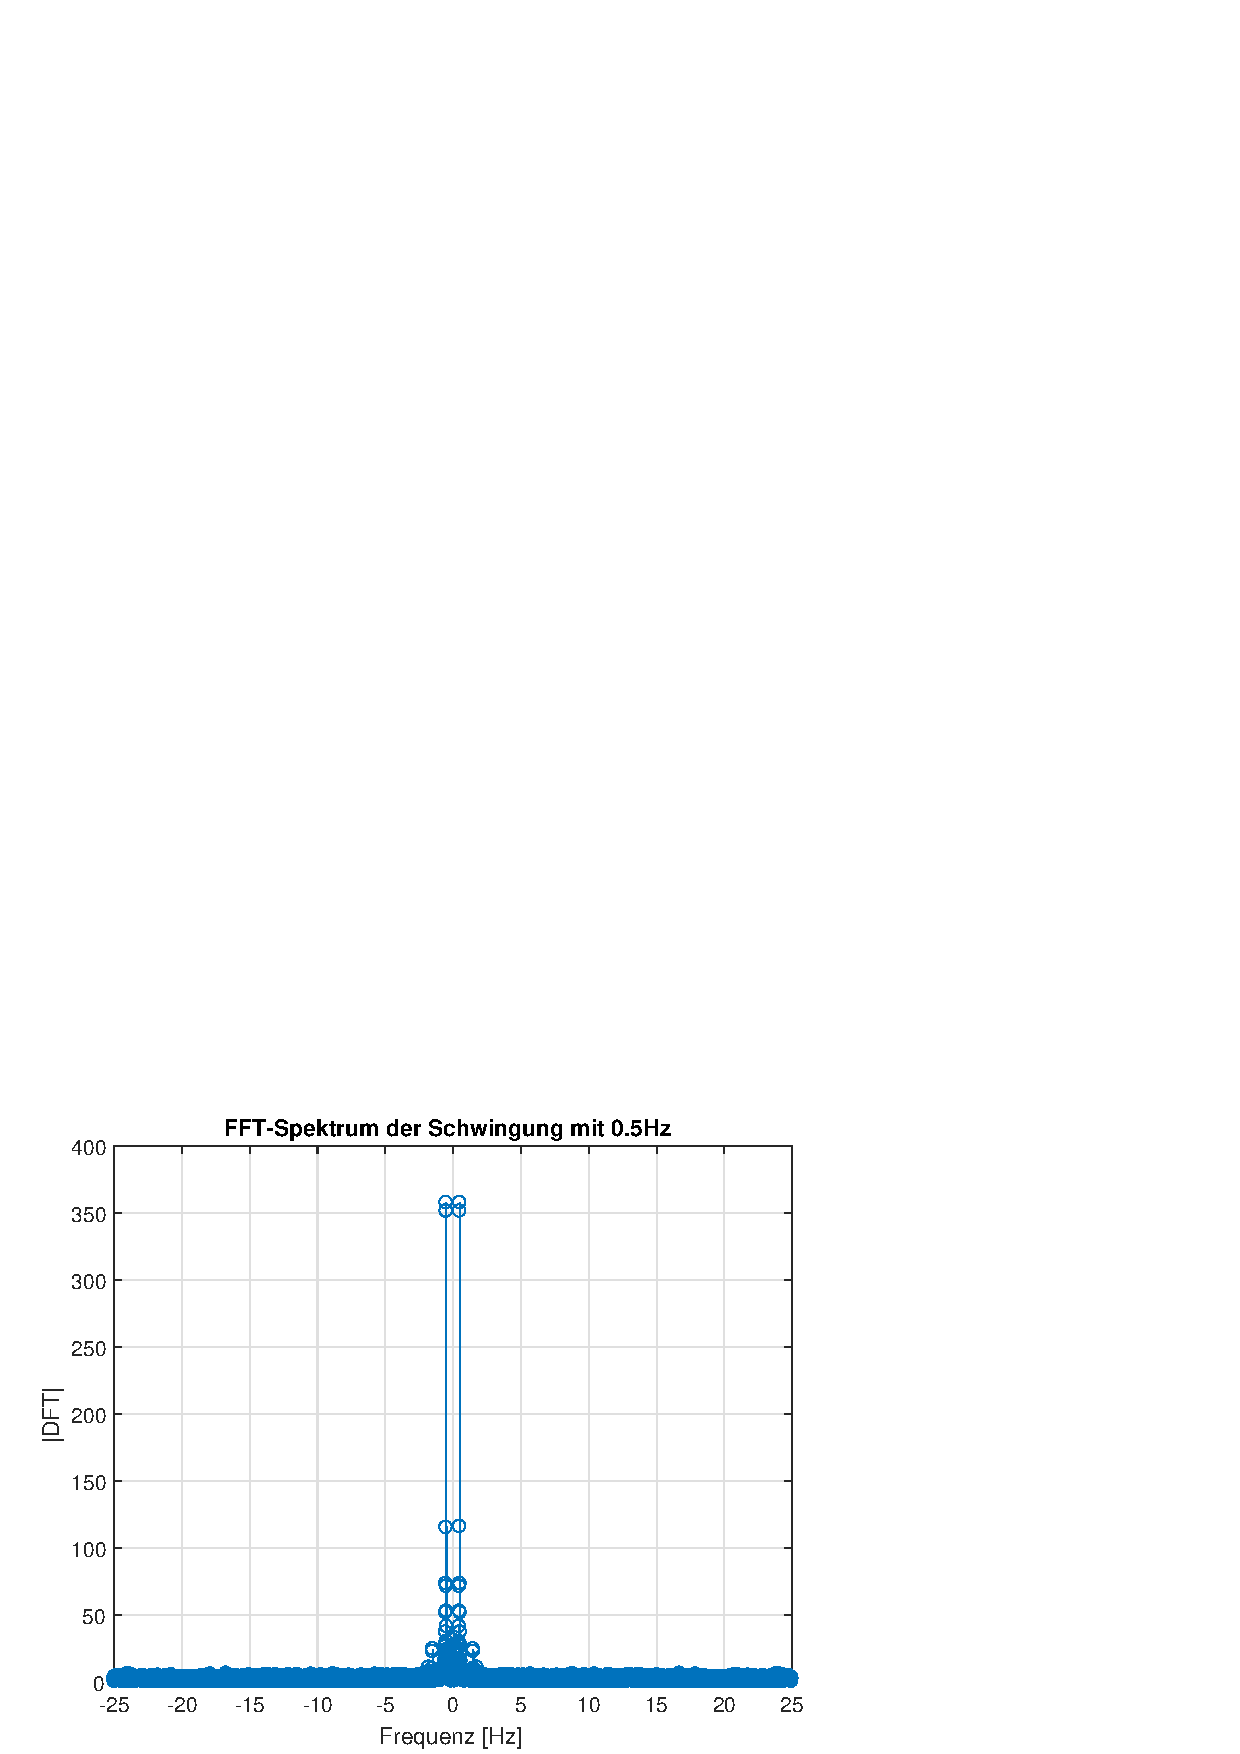
\includegraphics[width=0.5\linewidth]{img/dft_sinefreq_0_5}
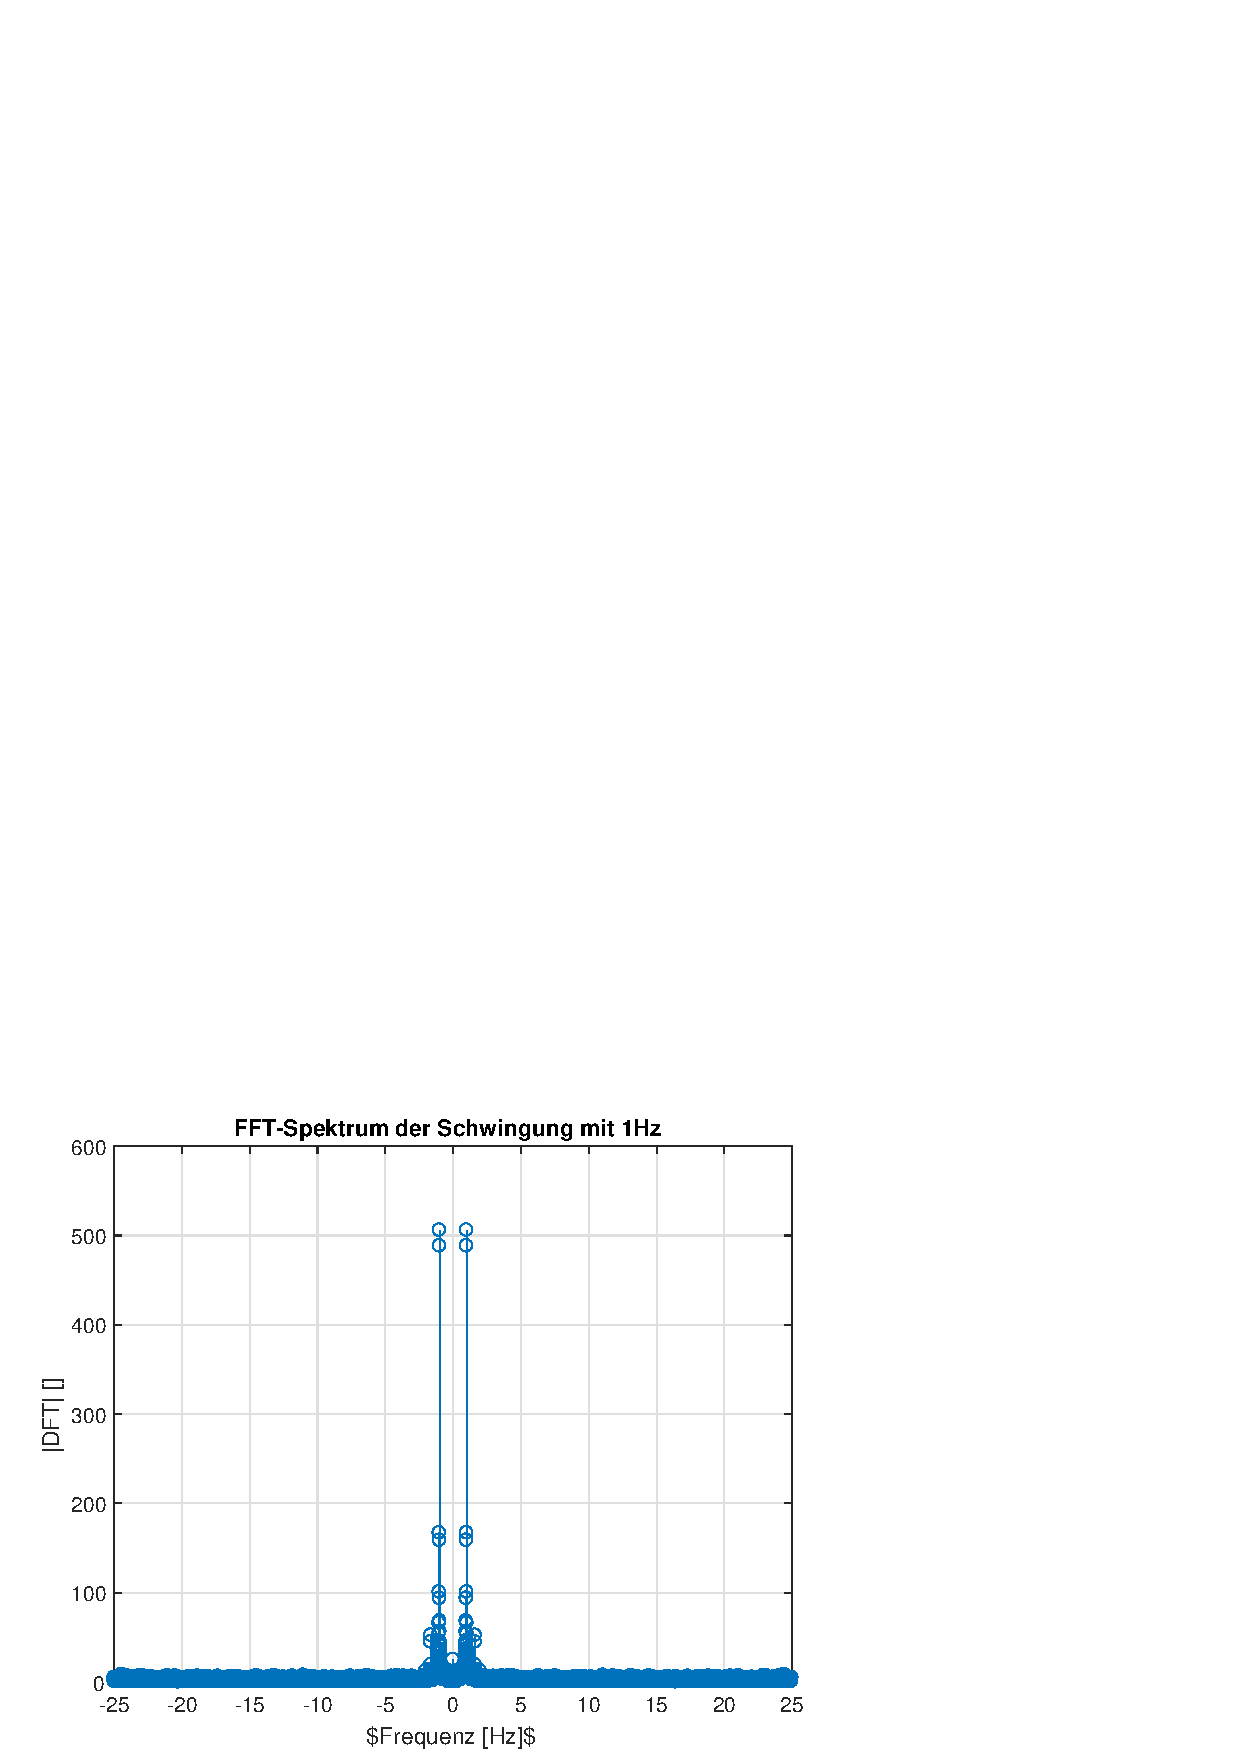
\includegraphics[width=0.5\linewidth]{img/dft_sinefreq_1}
\end{figure}
\begin{figure}[h!]
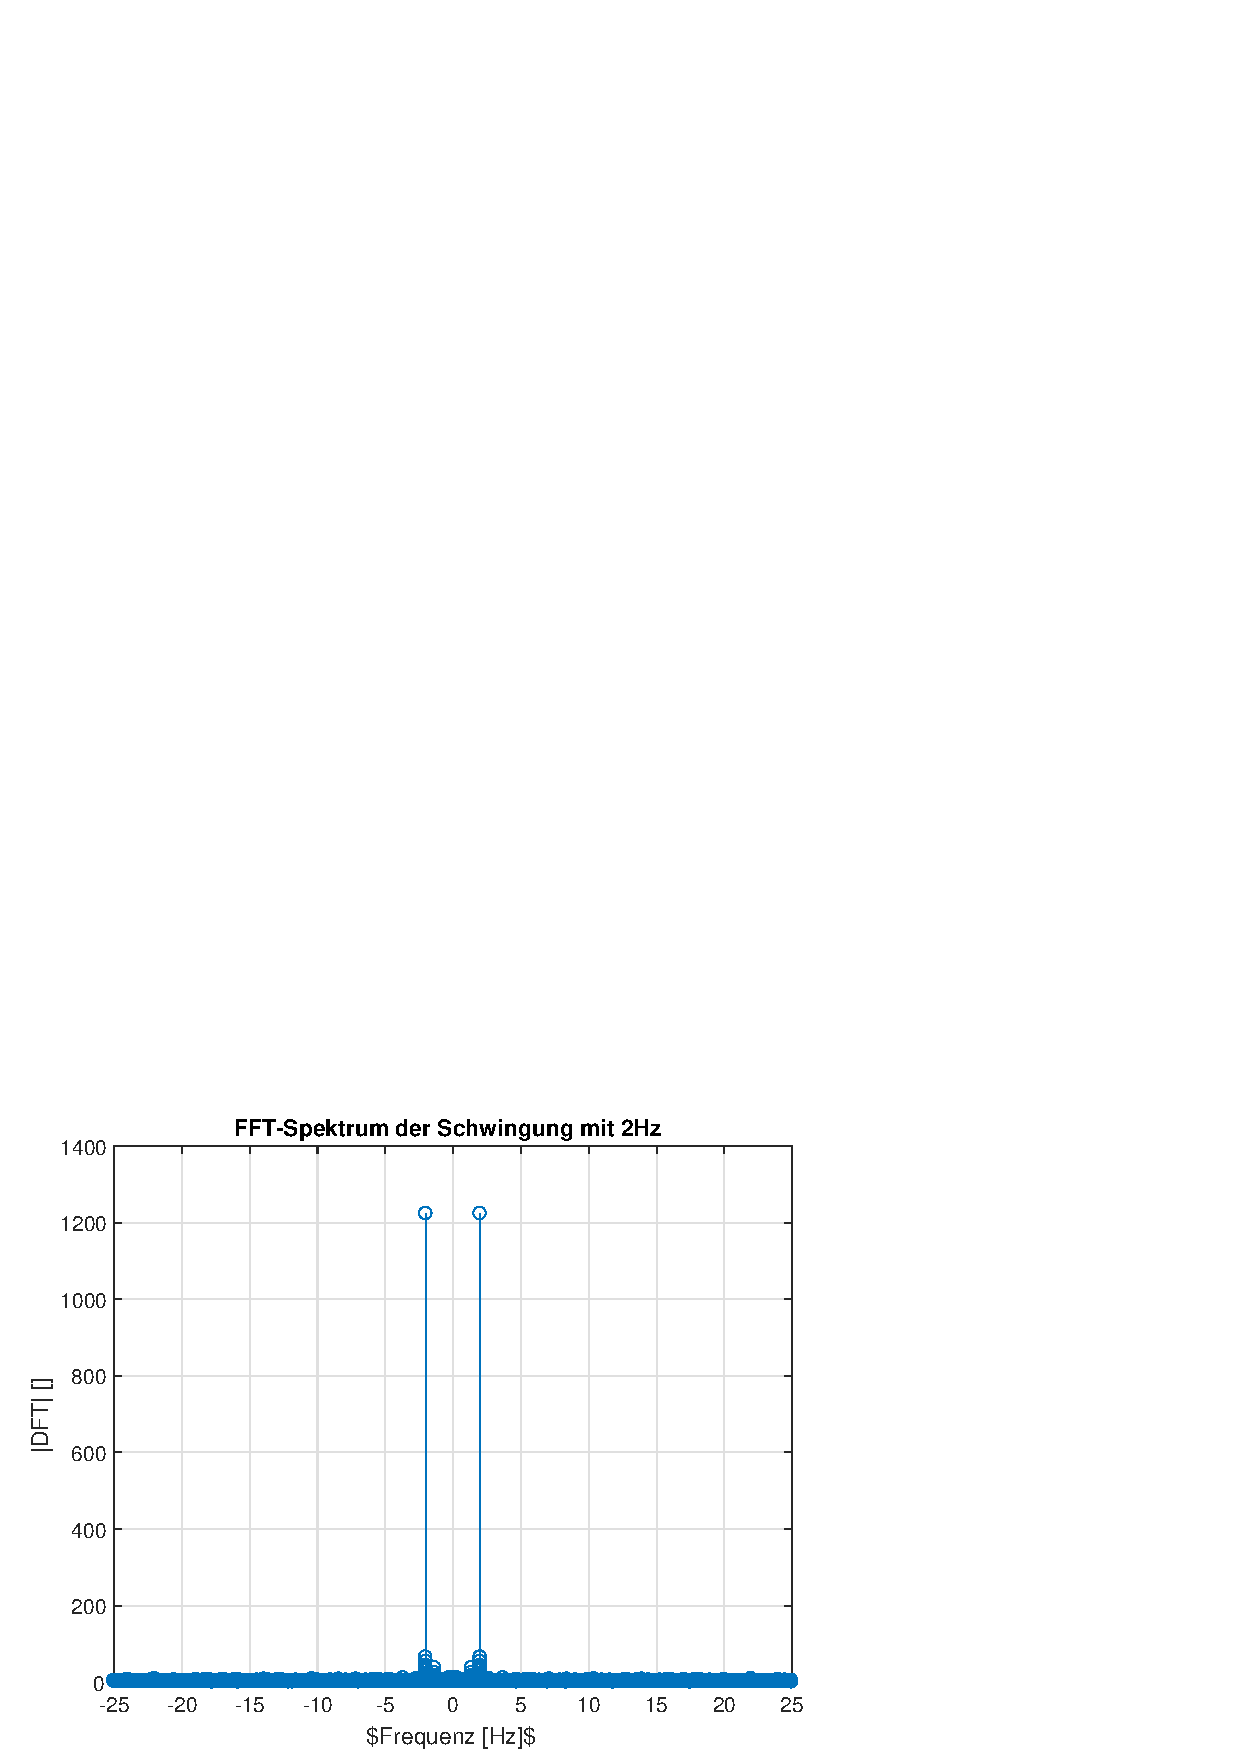
\includegraphics[width=0.5\linewidth]{img/dft_sinefreq_2}
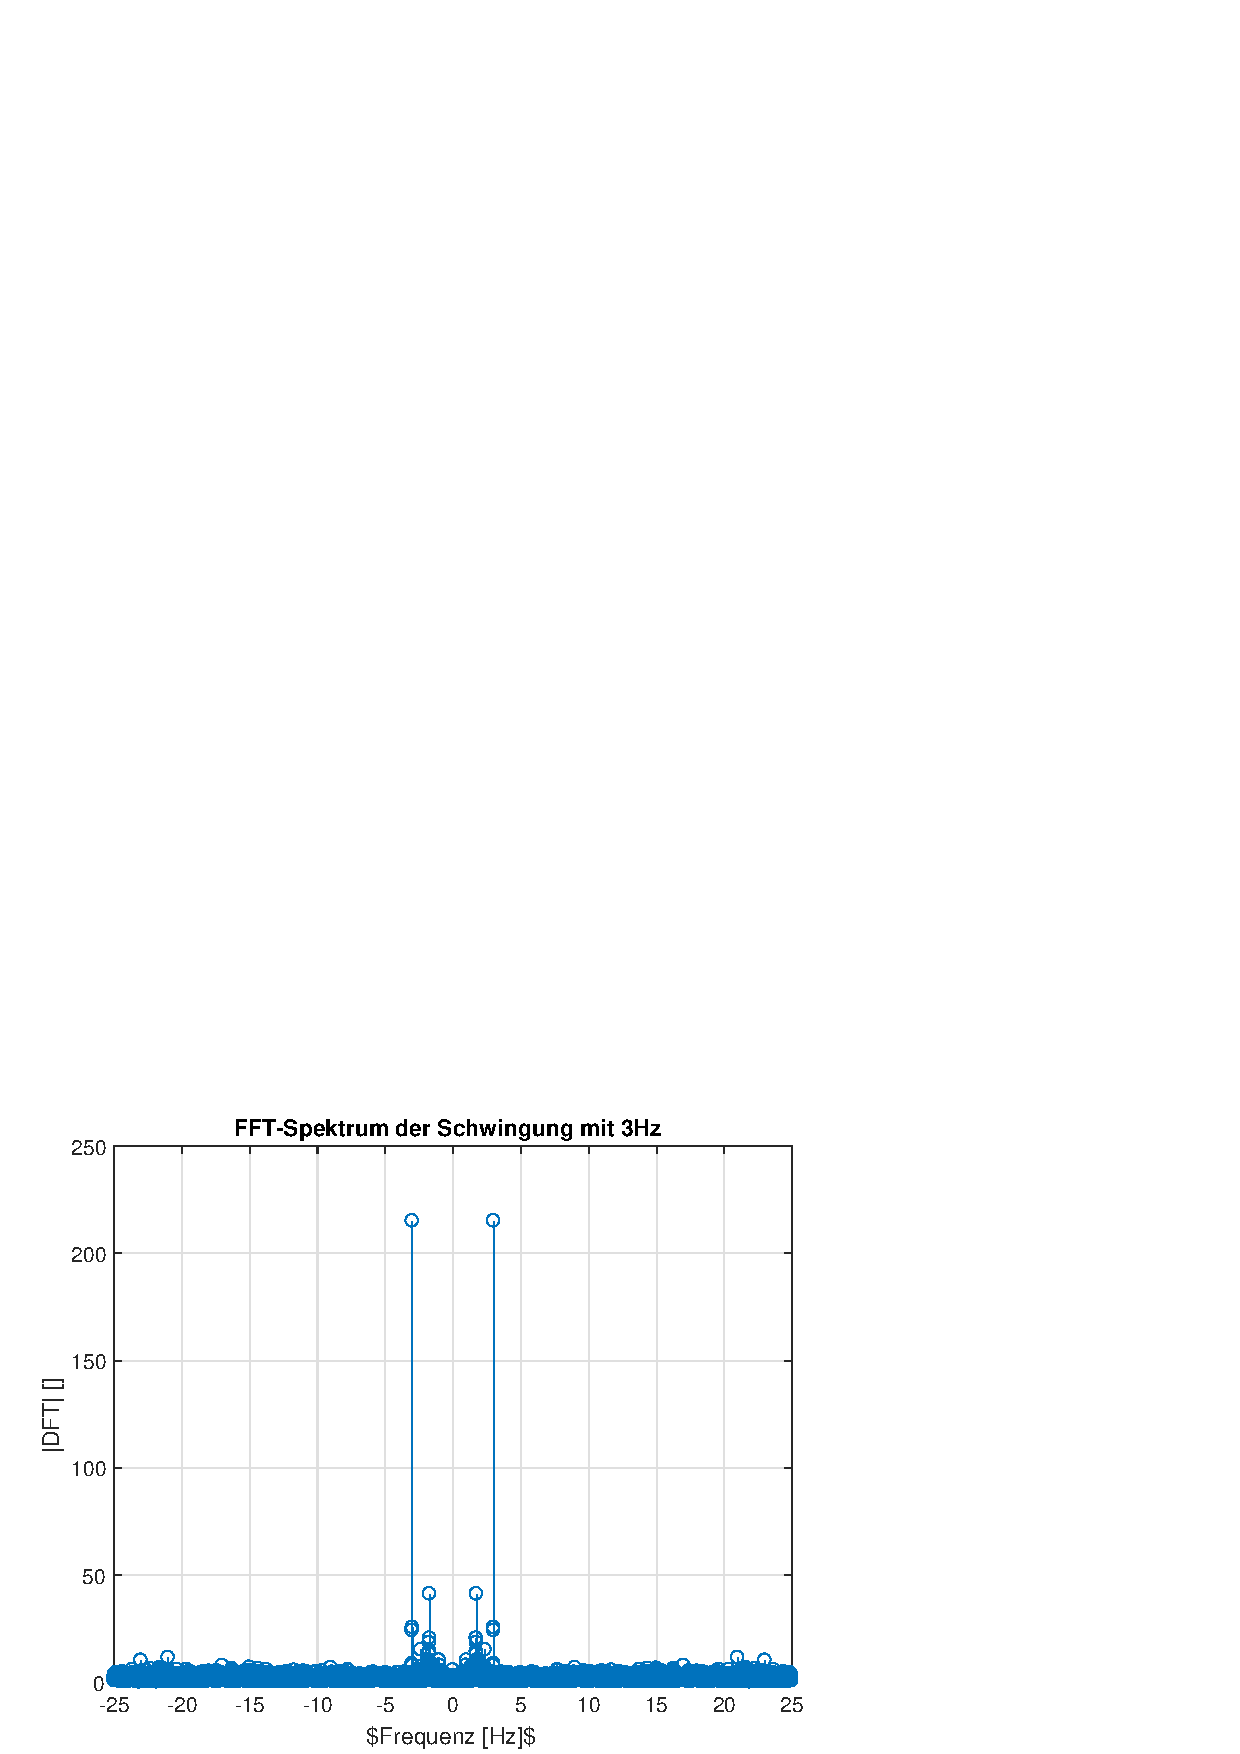
\includegraphics[width=0.5\linewidth]{img/dft_sinefreq_3}
\end{figure}
\begin{figure}[h!]
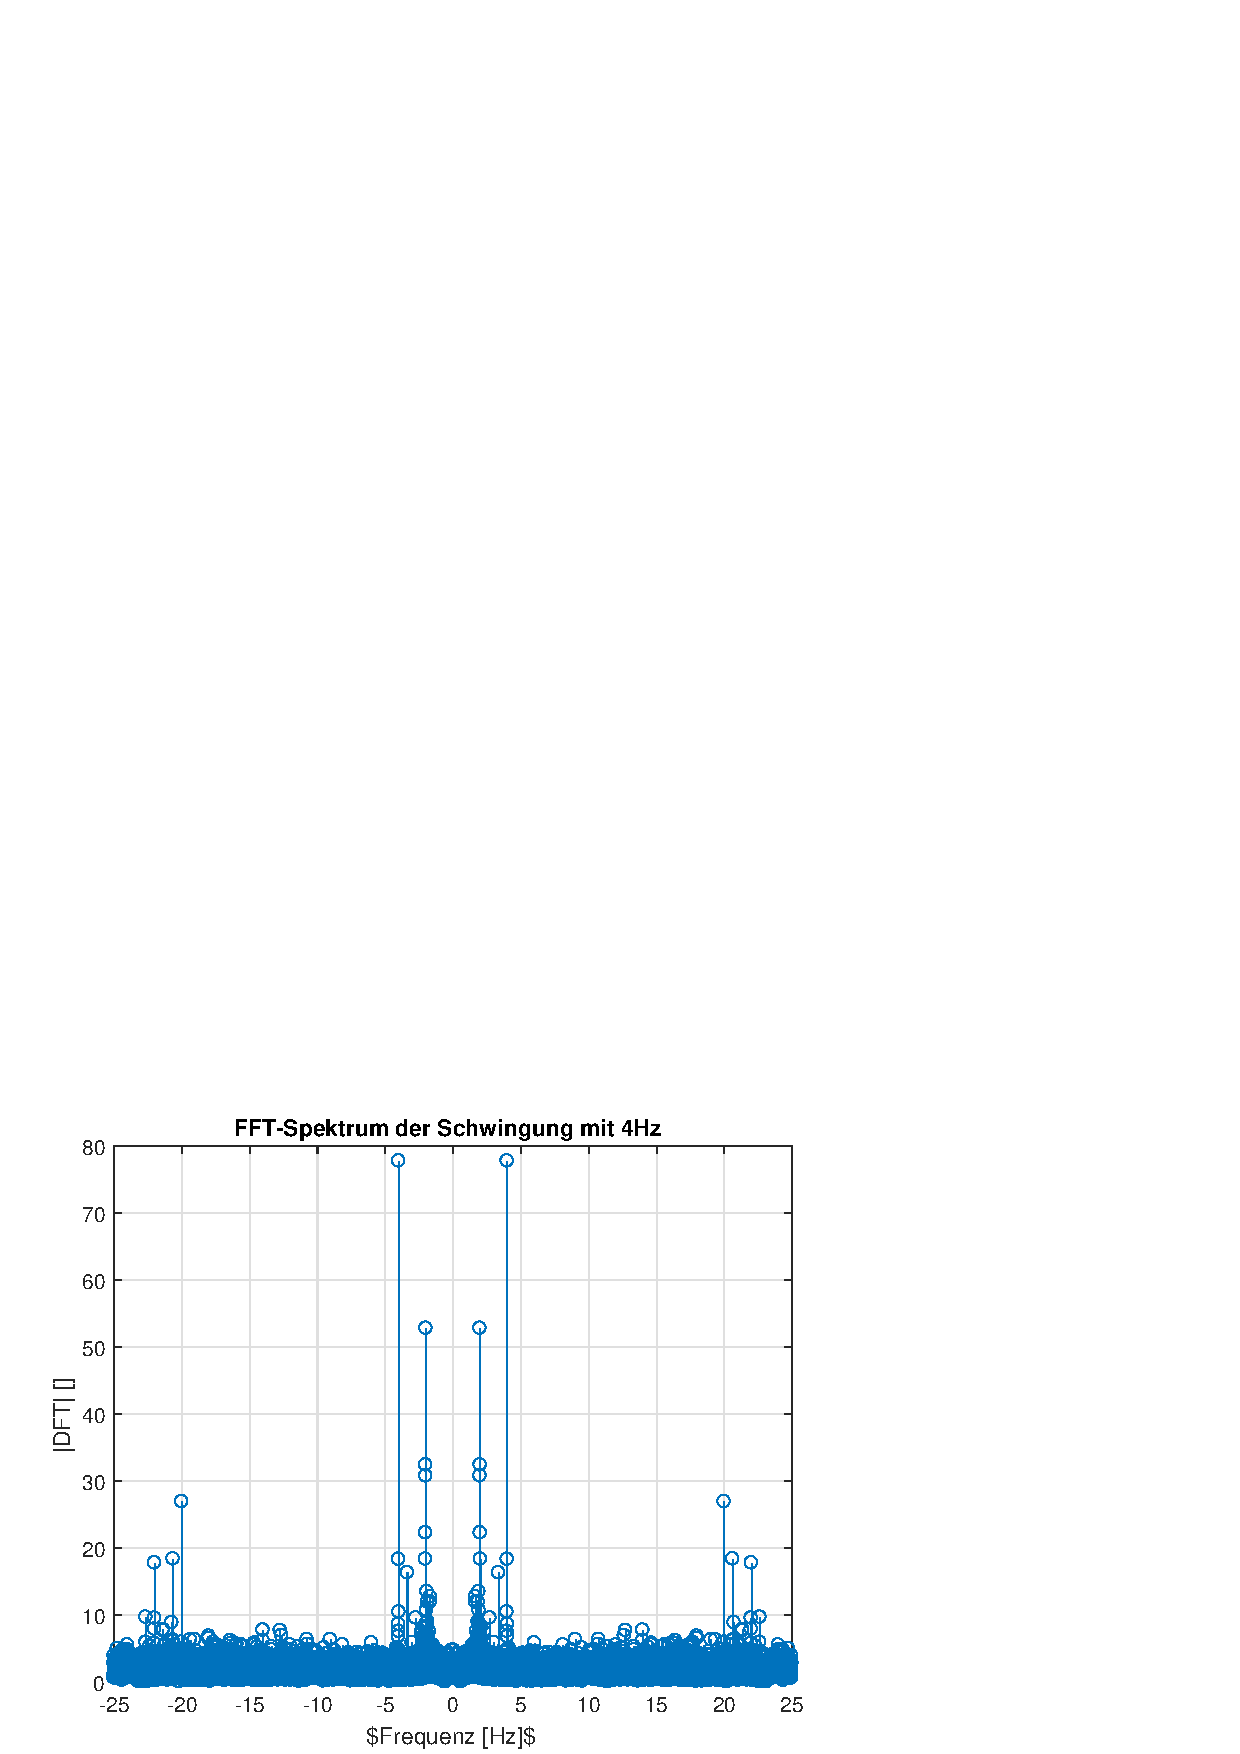
\includegraphics[width=0.5\linewidth]{img/dft_sinefreq_4}
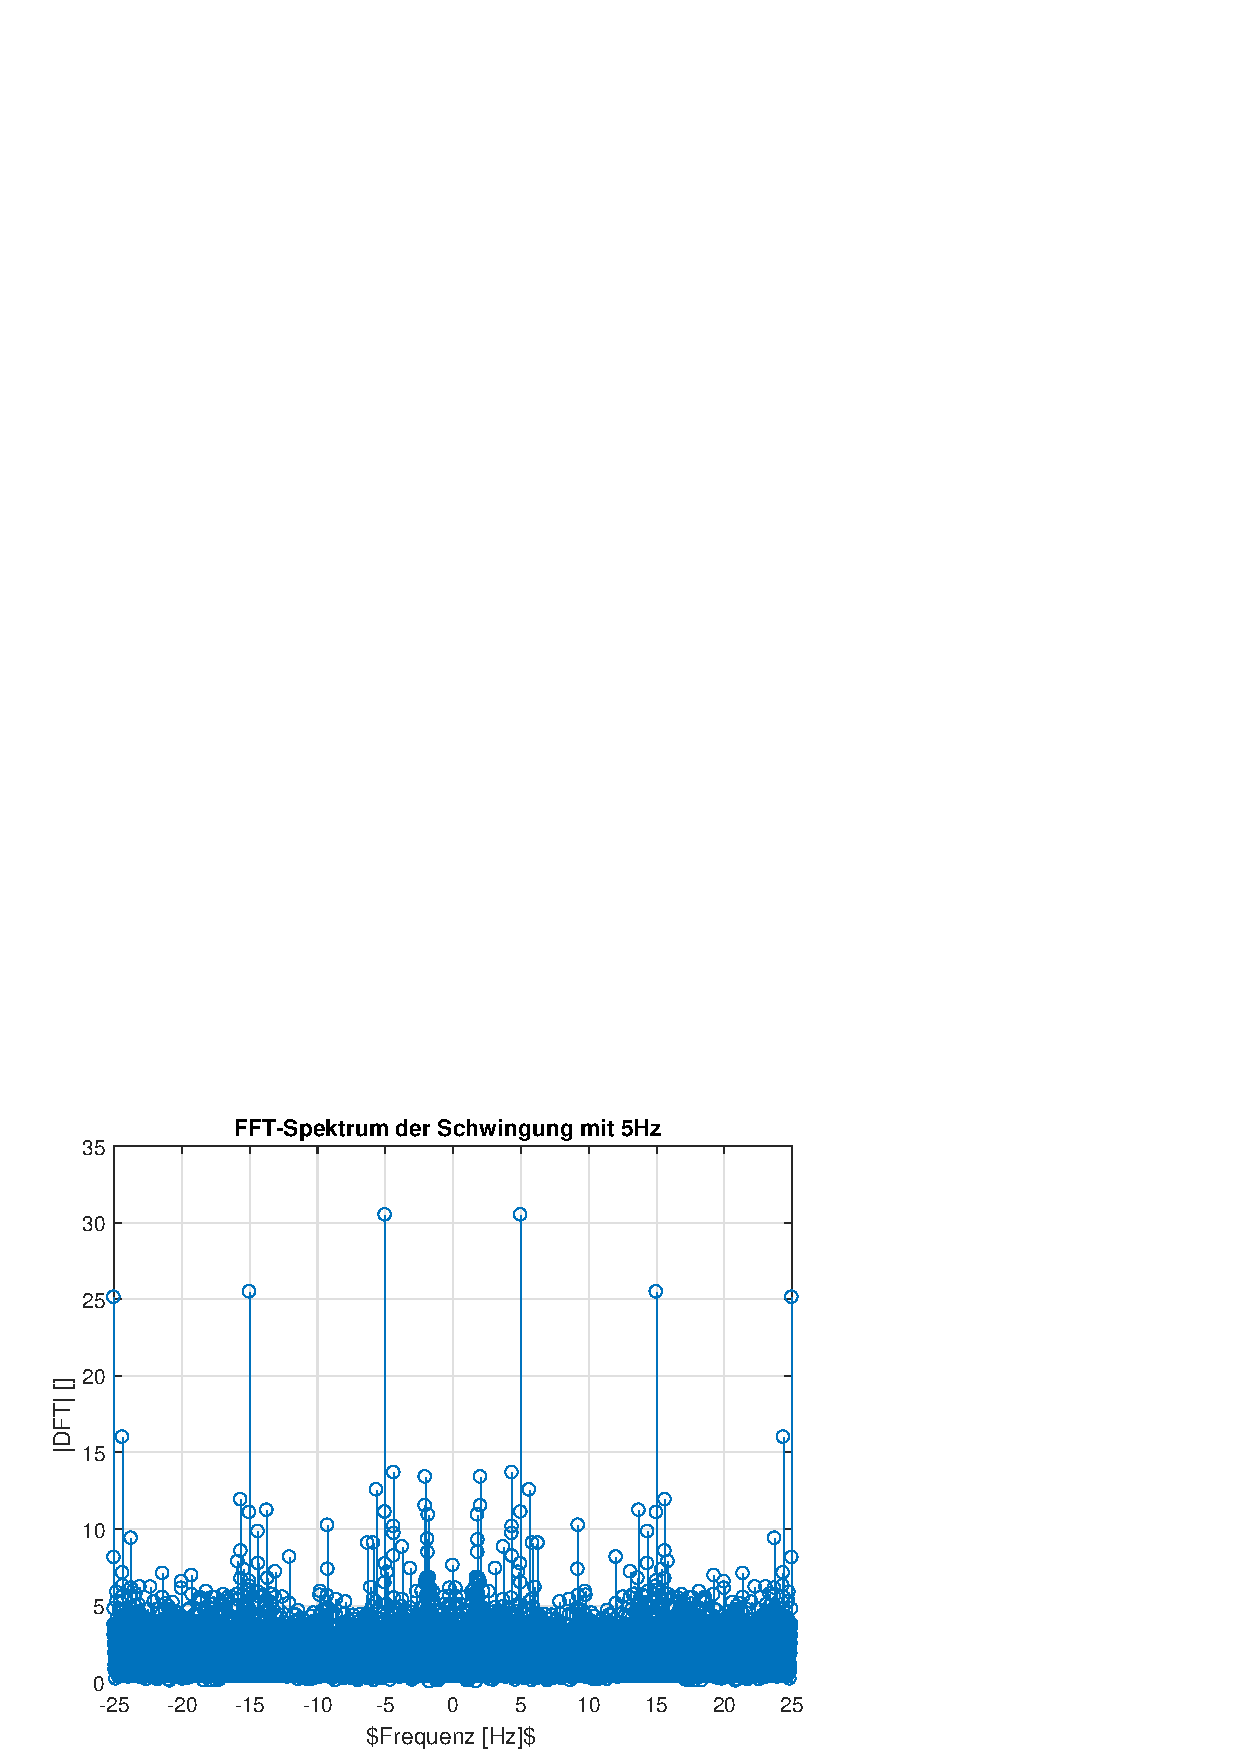
\includegraphics[width=0.5\linewidth]{img/dft_sinefreq_5}
\end{figure}
\newpage
\begin{figure}[h!]
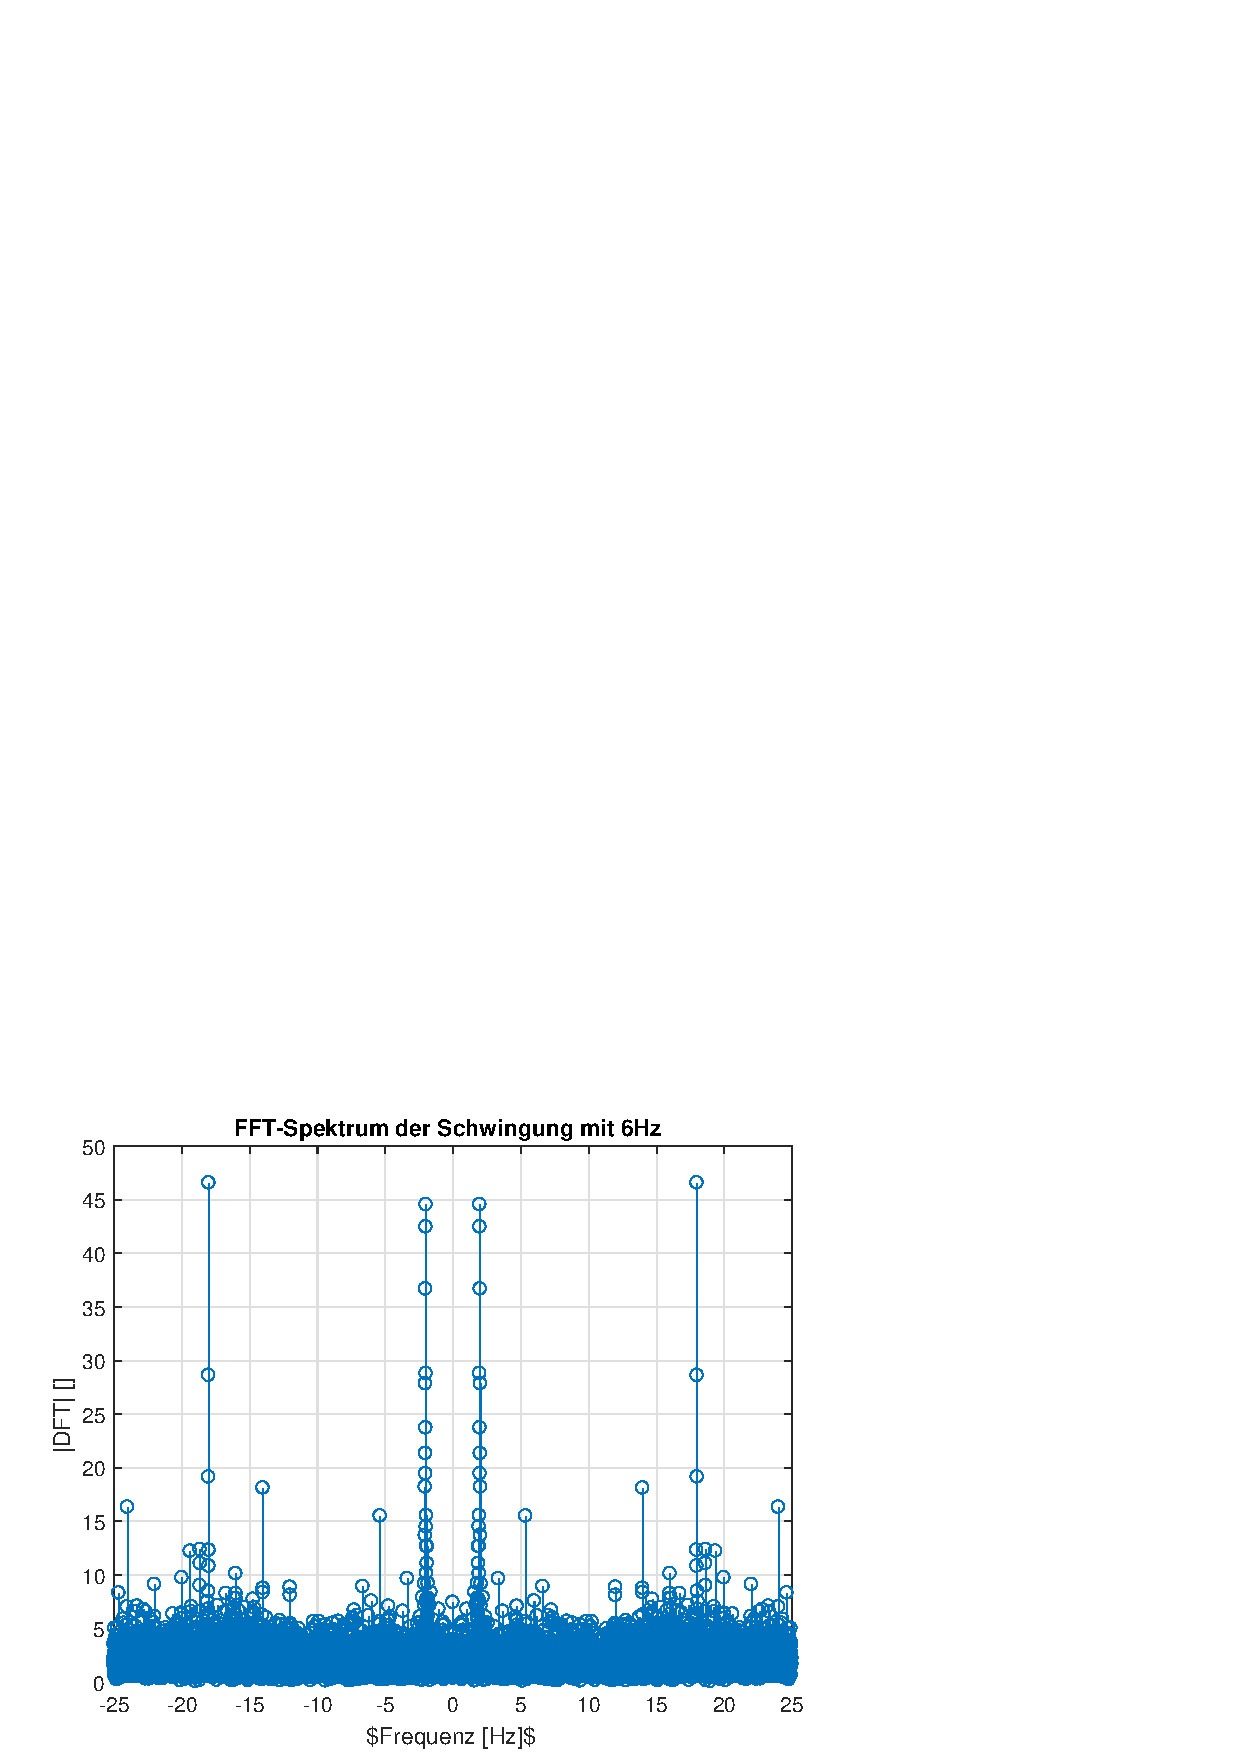
\includegraphics[width=0.5\linewidth]{img/dft_sinefreq_6}
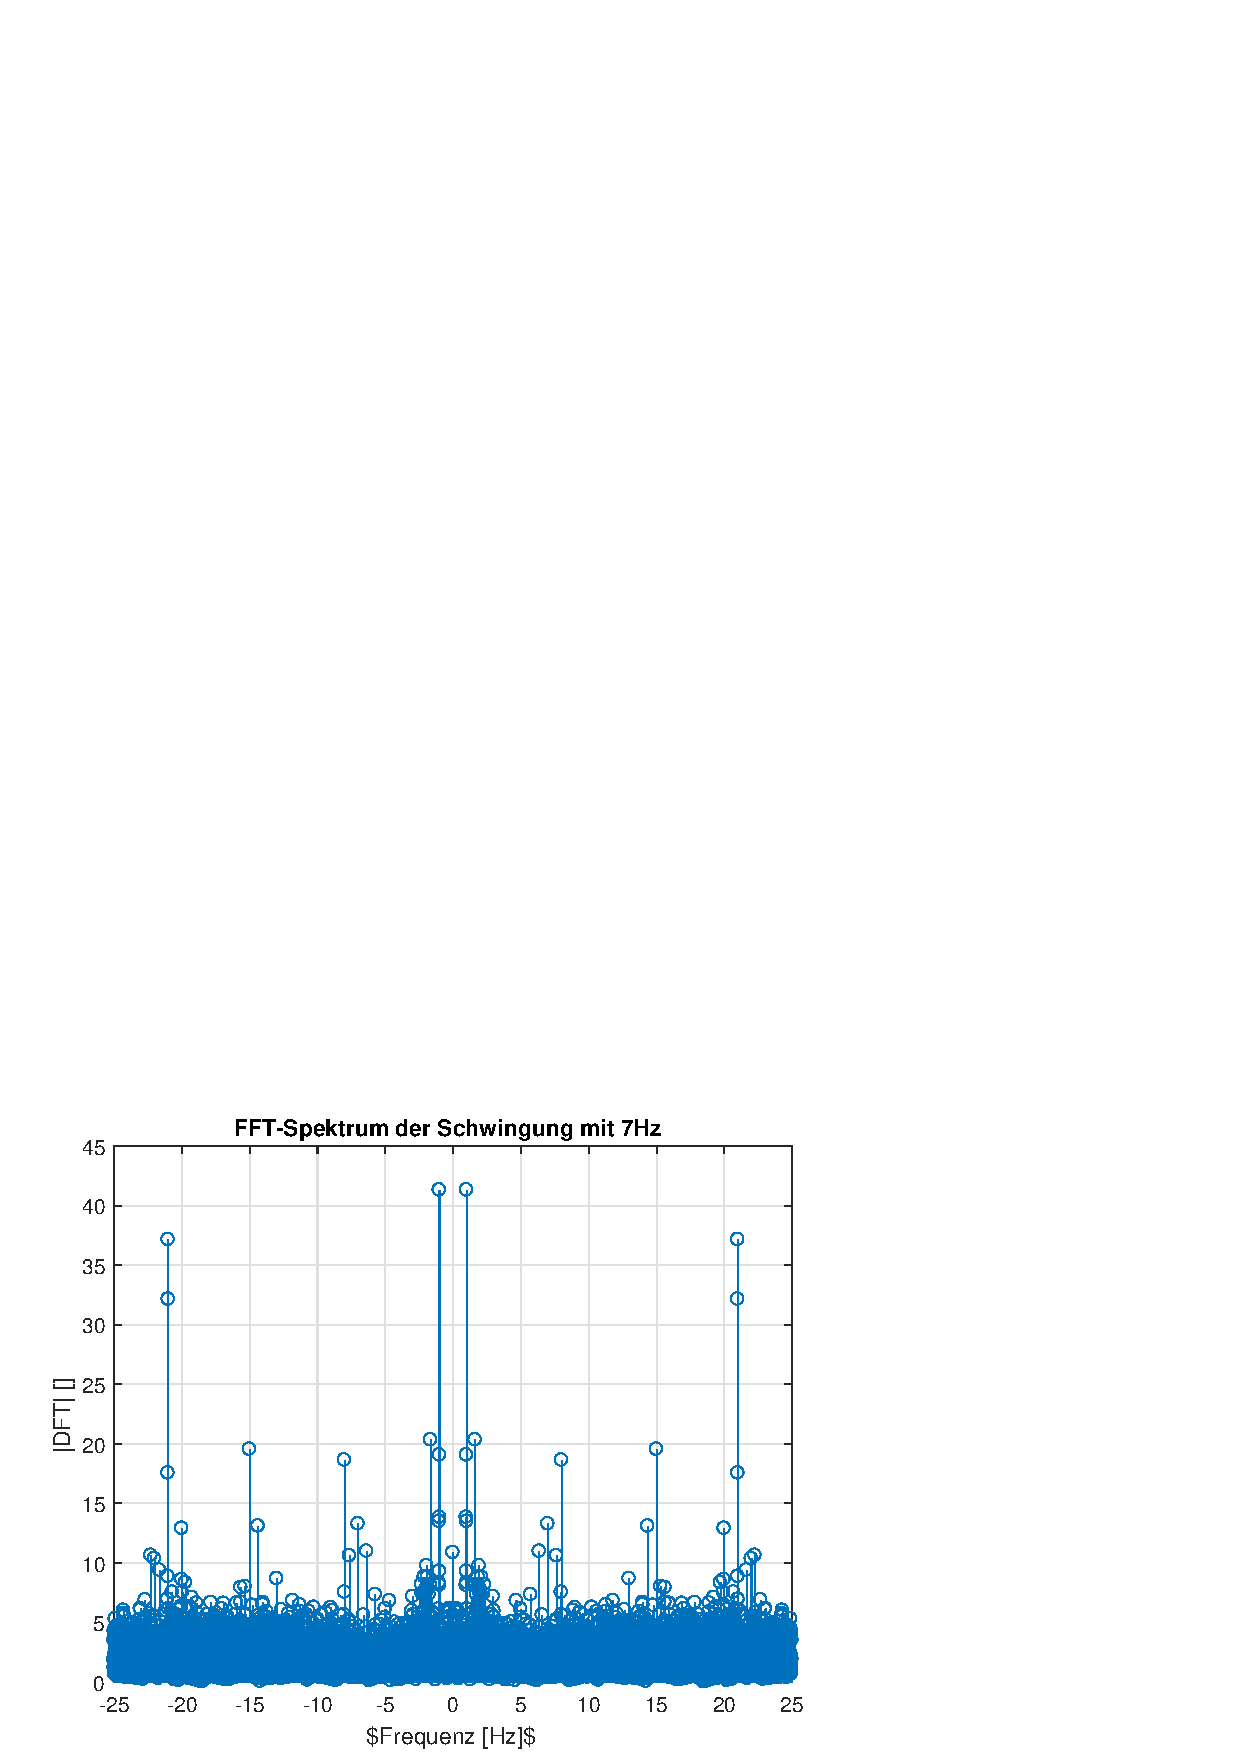
\includegraphics[width=0.5\linewidth]{img/dft_sinefreq_7}
\end{figure}
\begin{figure}[h!]
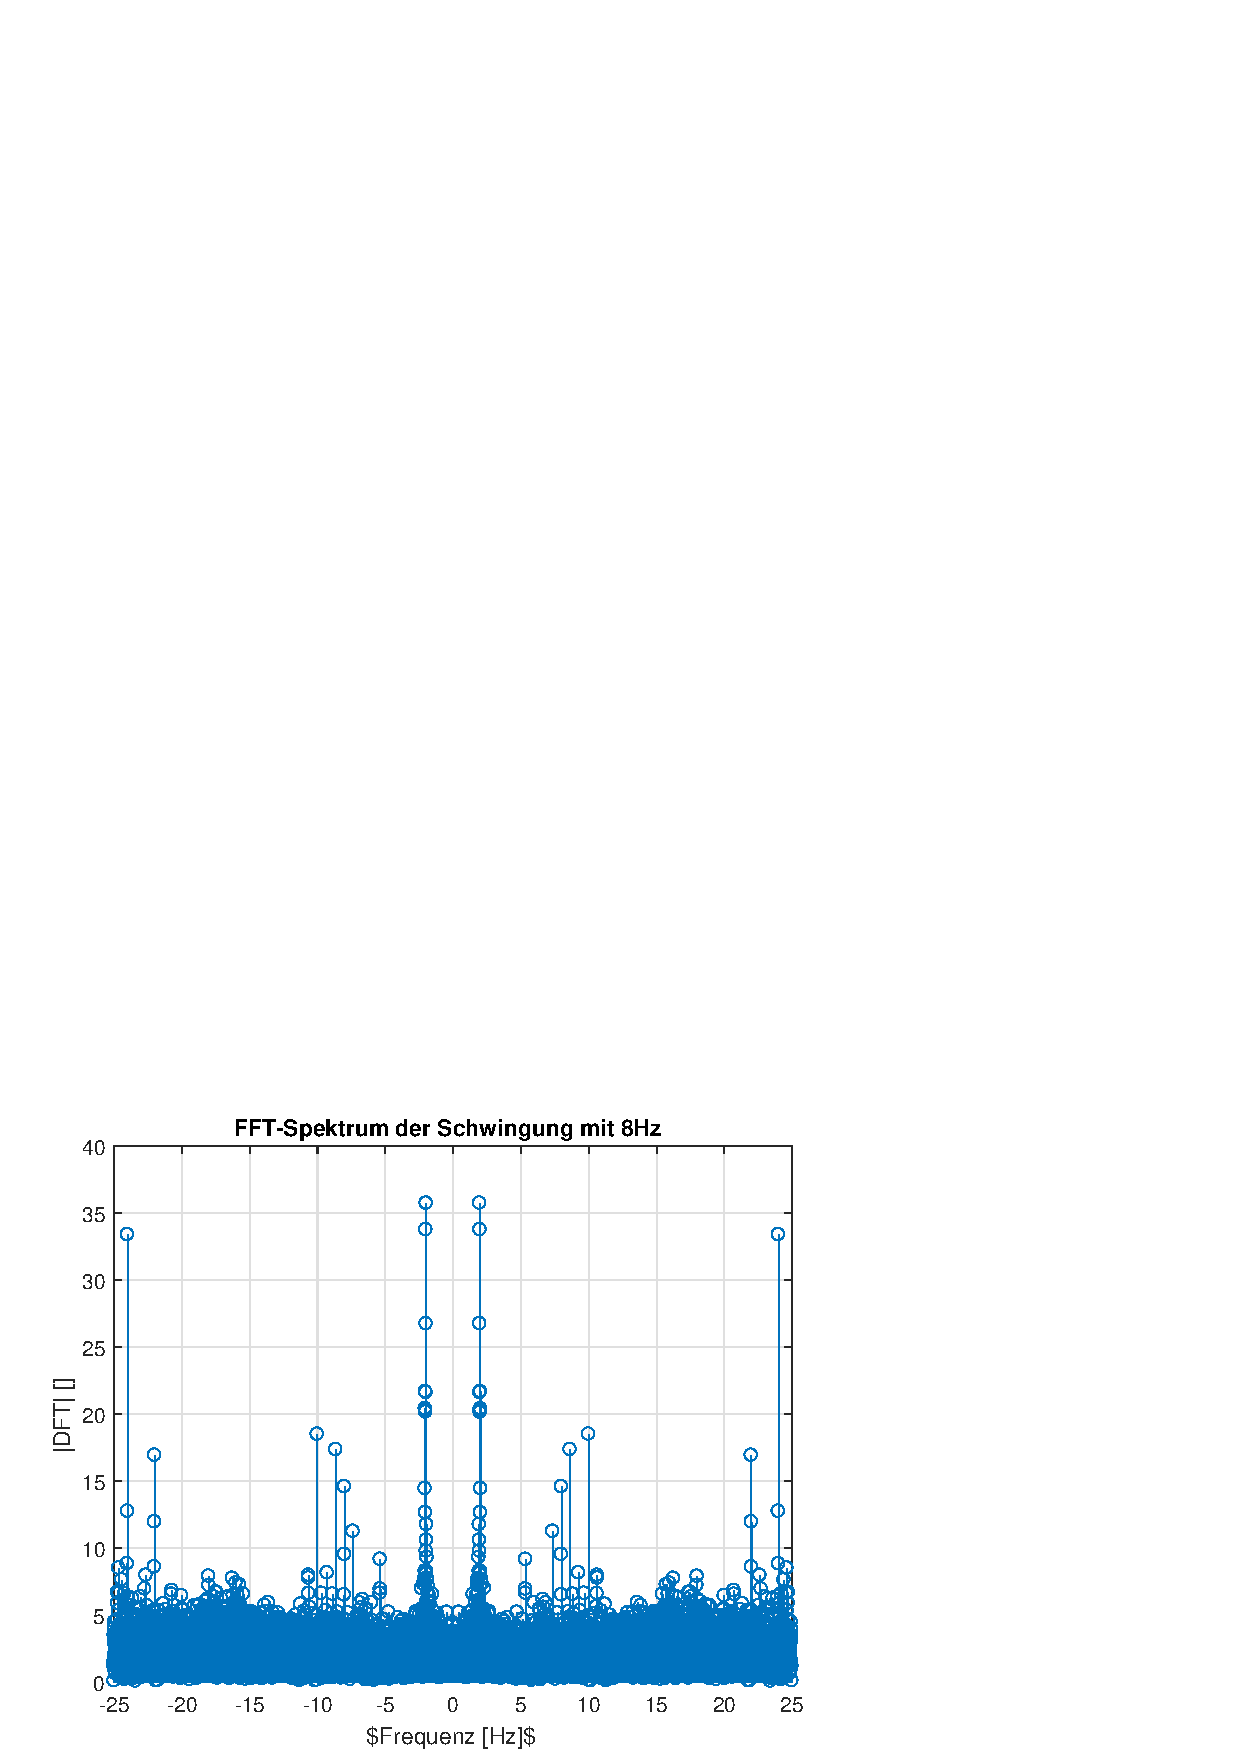
\includegraphics[width=0.5\linewidth]{img/dft_sinefreq_8}
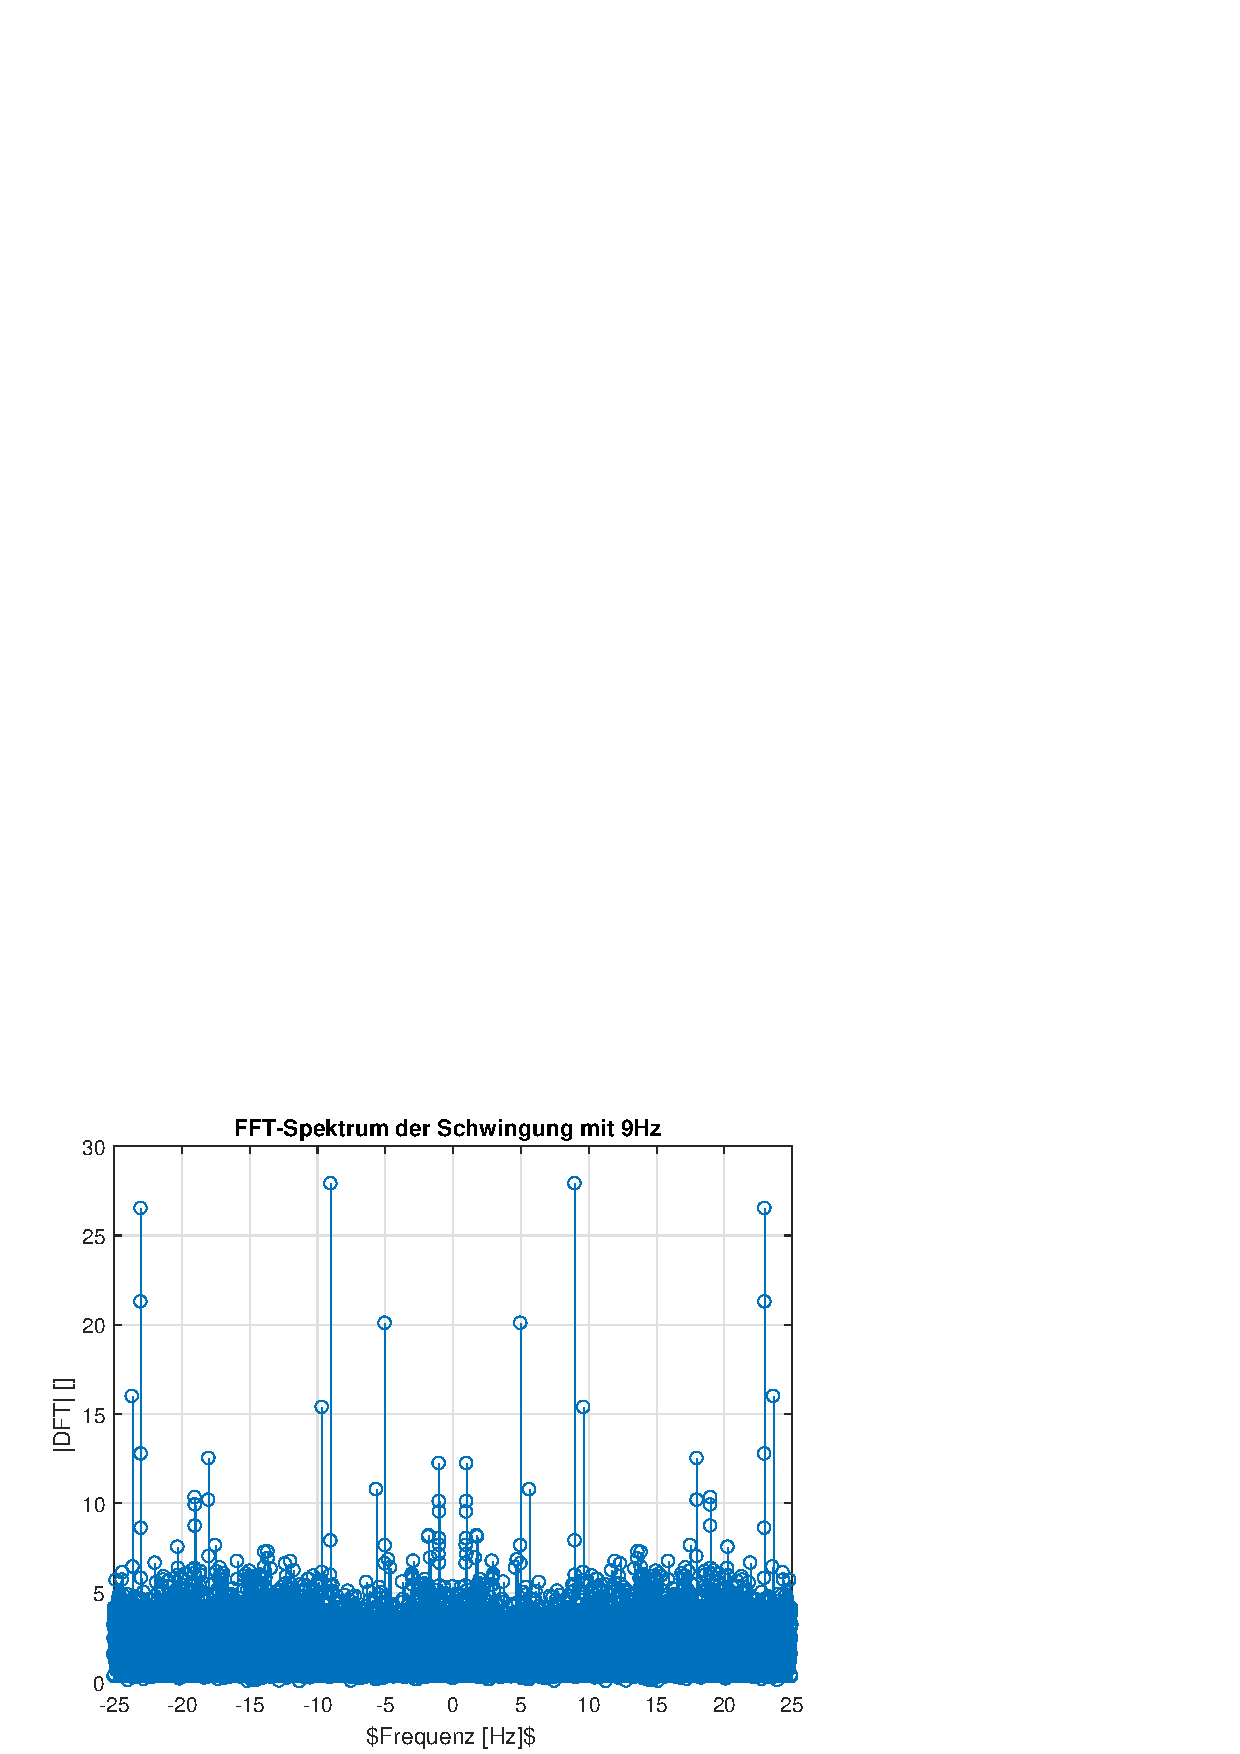
\includegraphics[width=0.5\linewidth]{img/dft_sinefreq_9}
\end{figure}
\begin{figure}[h!]
\centering
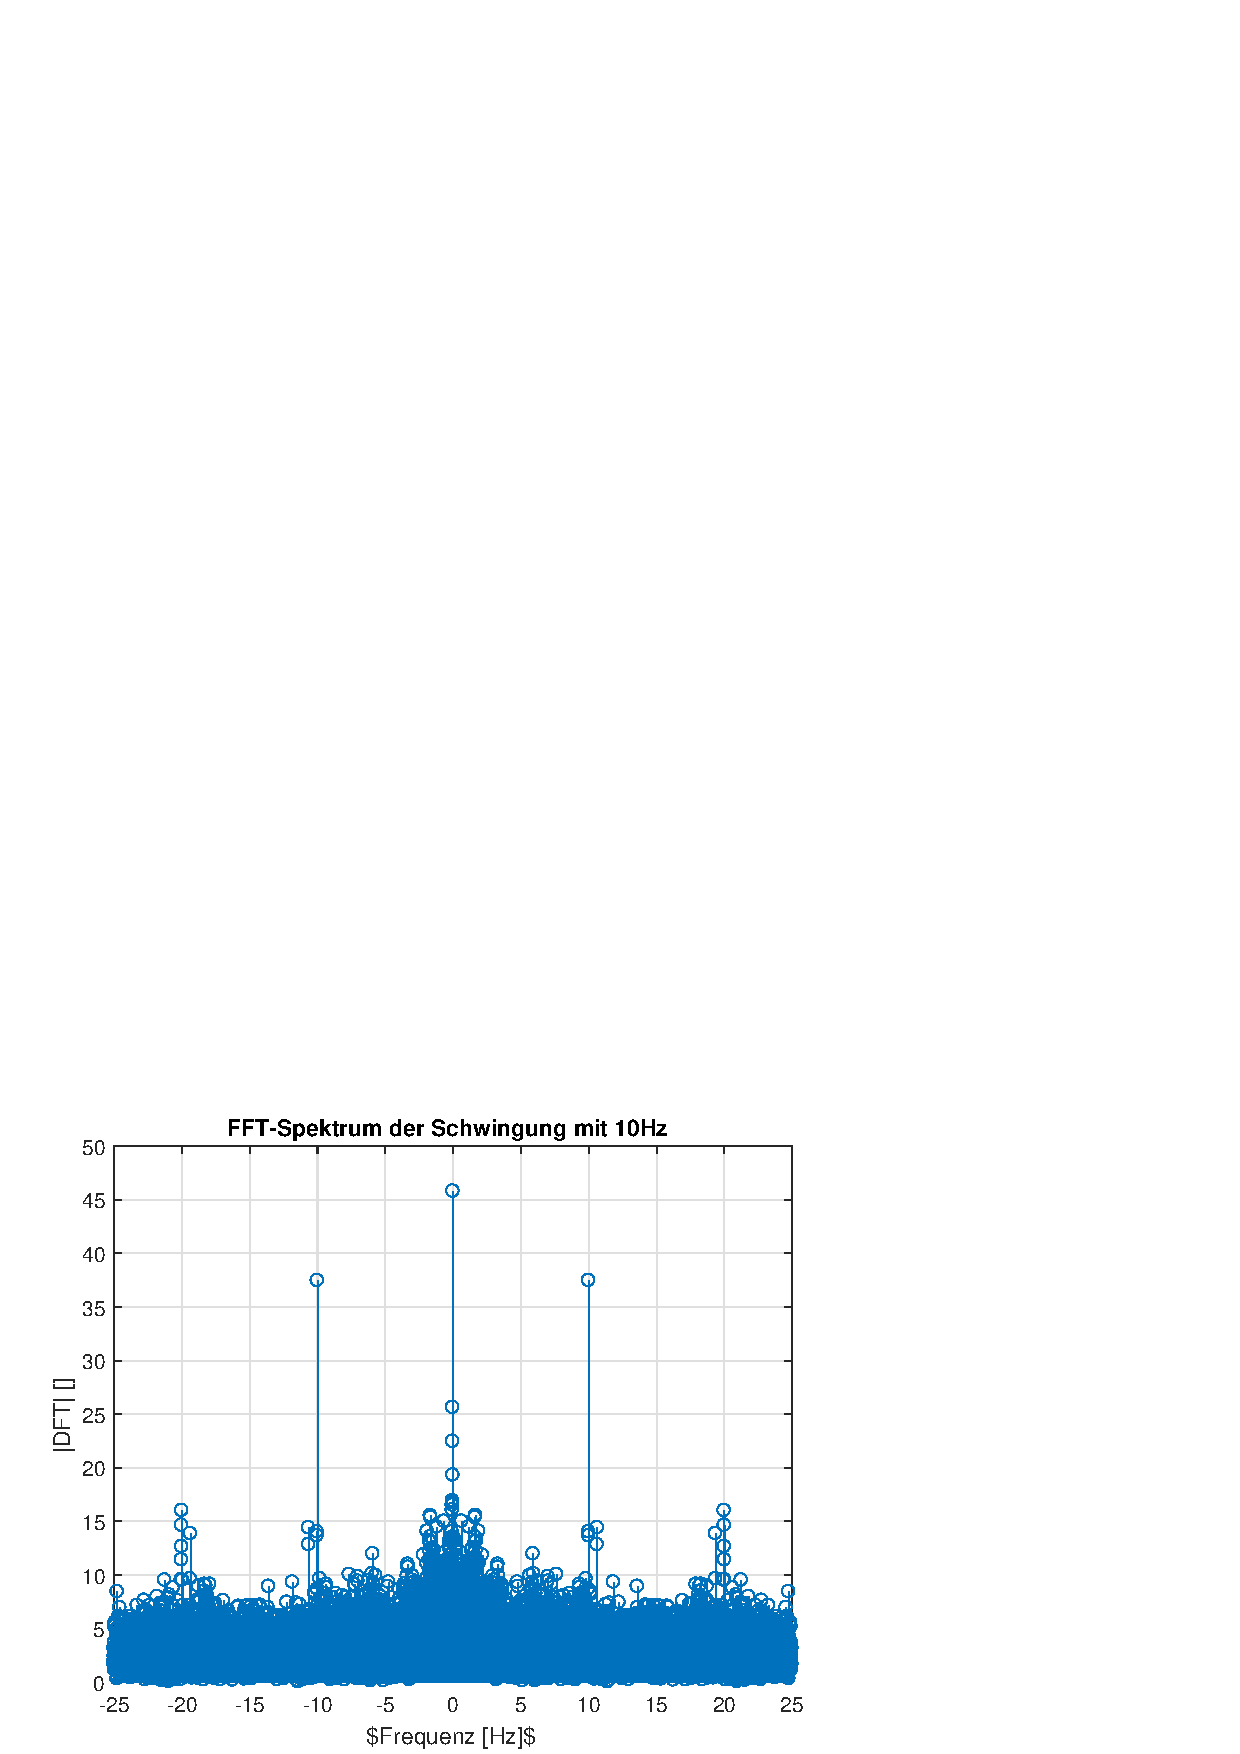
\includegraphics[width=0.5\linewidth]{img/dft_sinefreq_10}
\end{figure}

\newpage

\subsection{Leistungsdichtespektren von $\varphi$ bei $T_M = sin(2\pi\cdot f\cdot t)$}
\begin{figure}[h!]
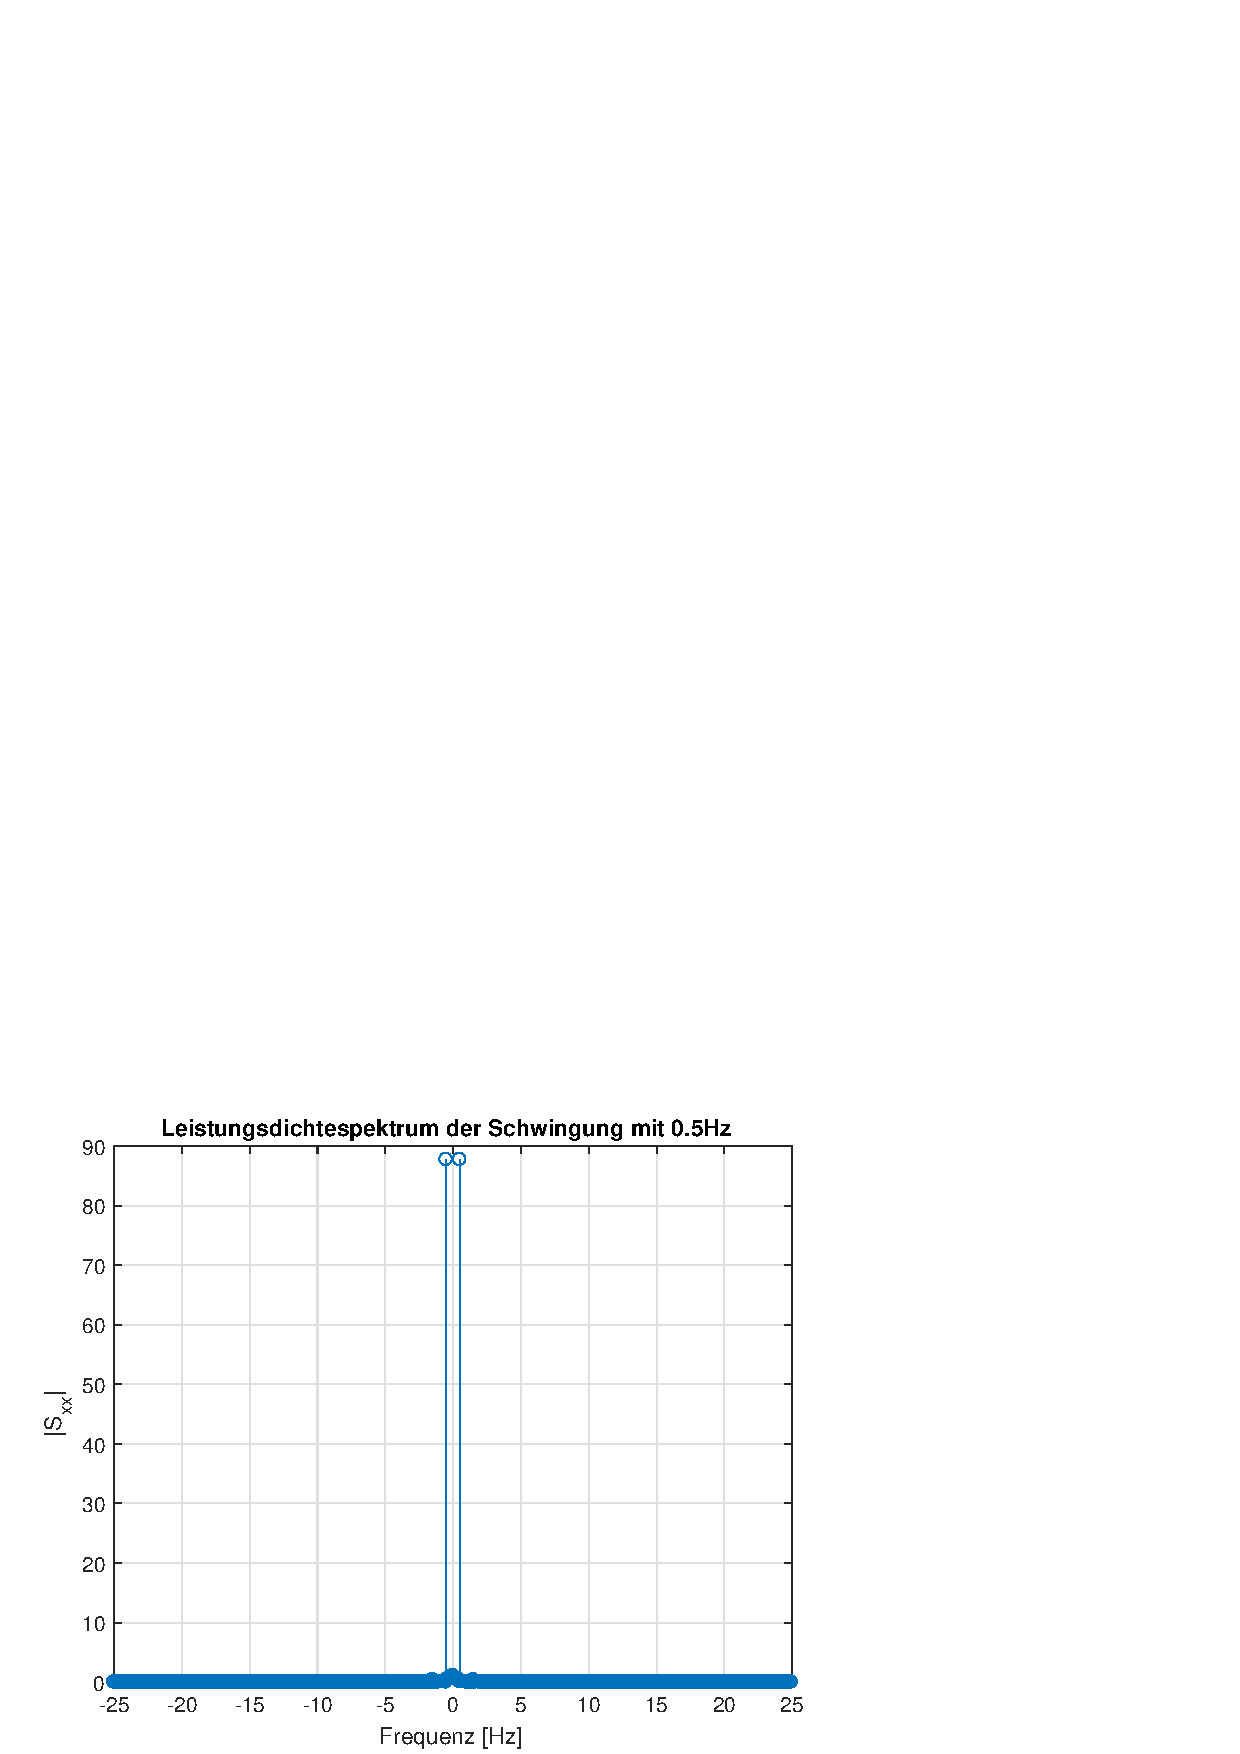
\includegraphics[width=0.5\linewidth]{img/lds_sinefreq_0_5}
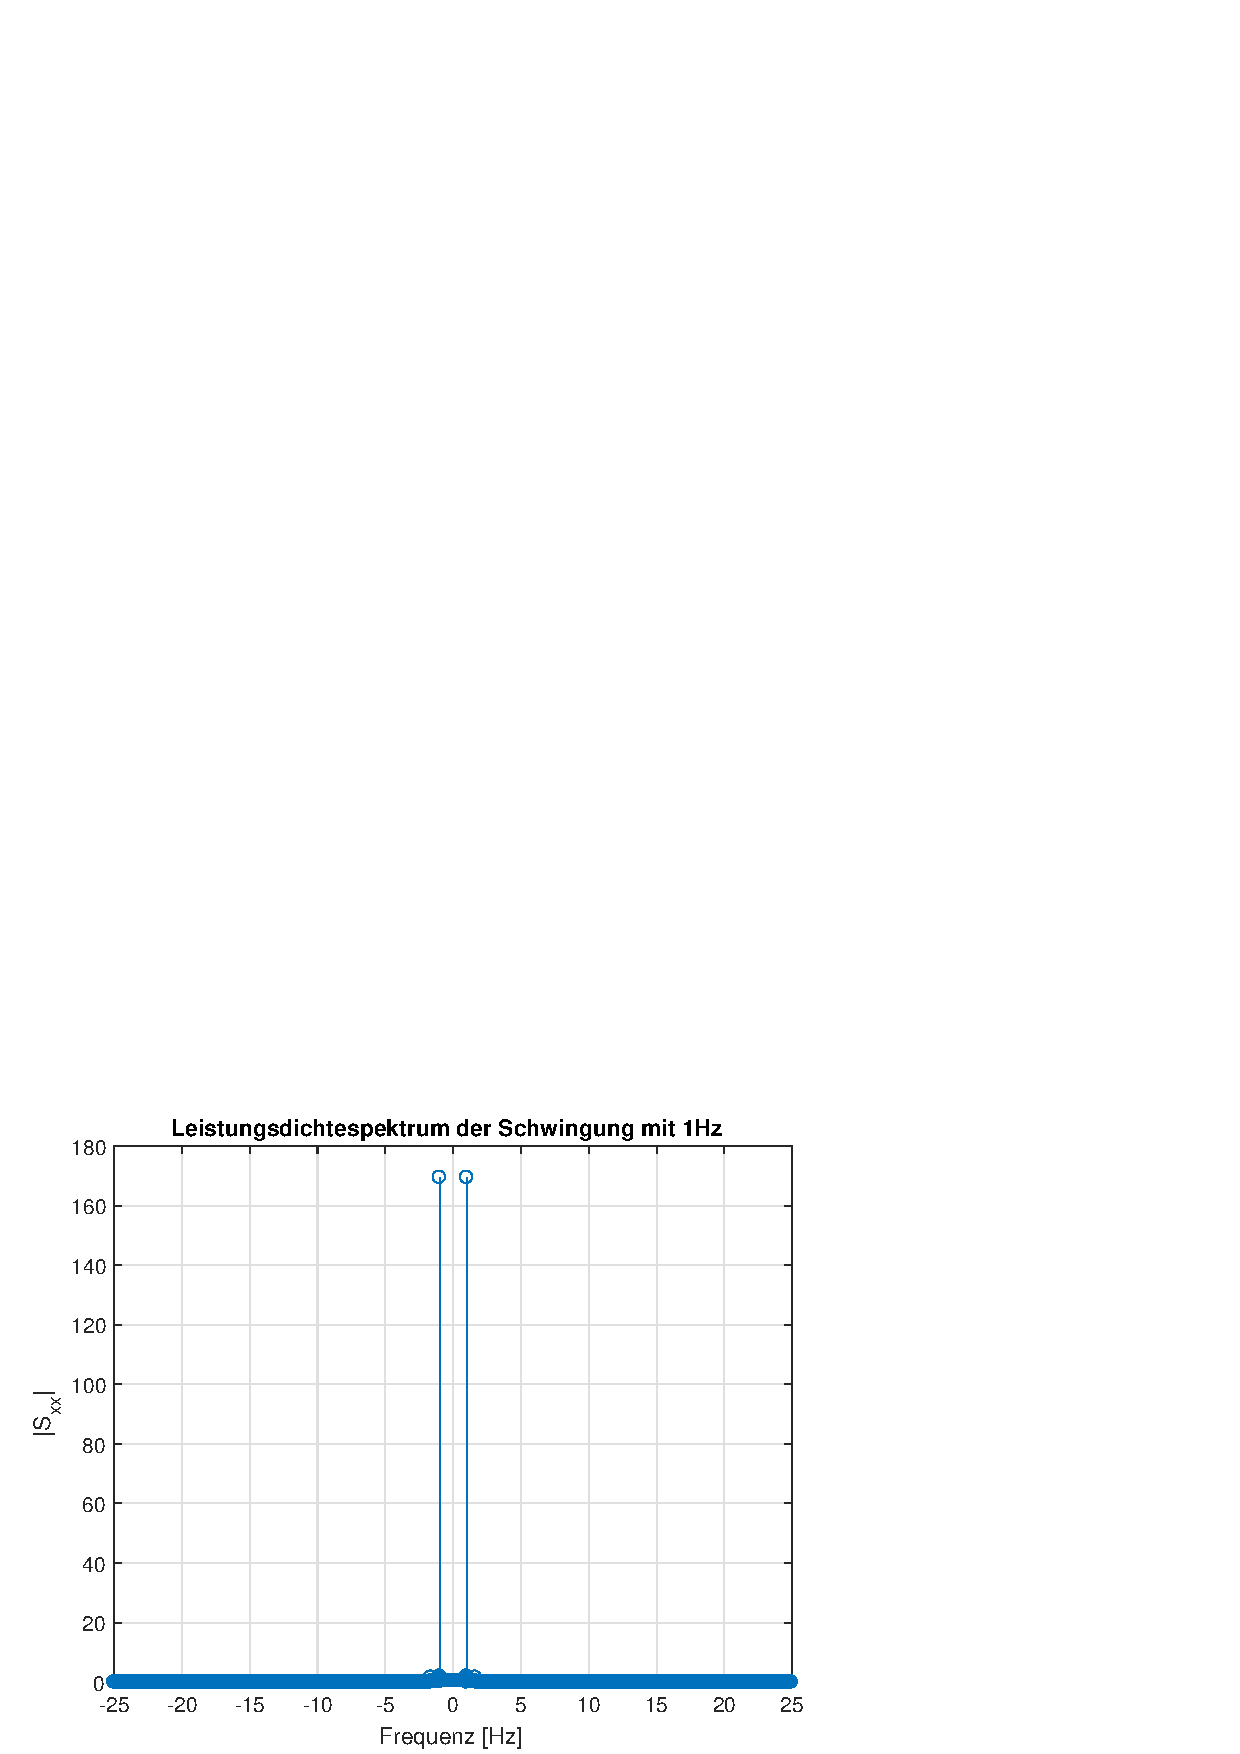
\includegraphics[width=0.5\linewidth]{img/lds_sinefreq_1}
\end{figure}
\begin{figure}[h!]
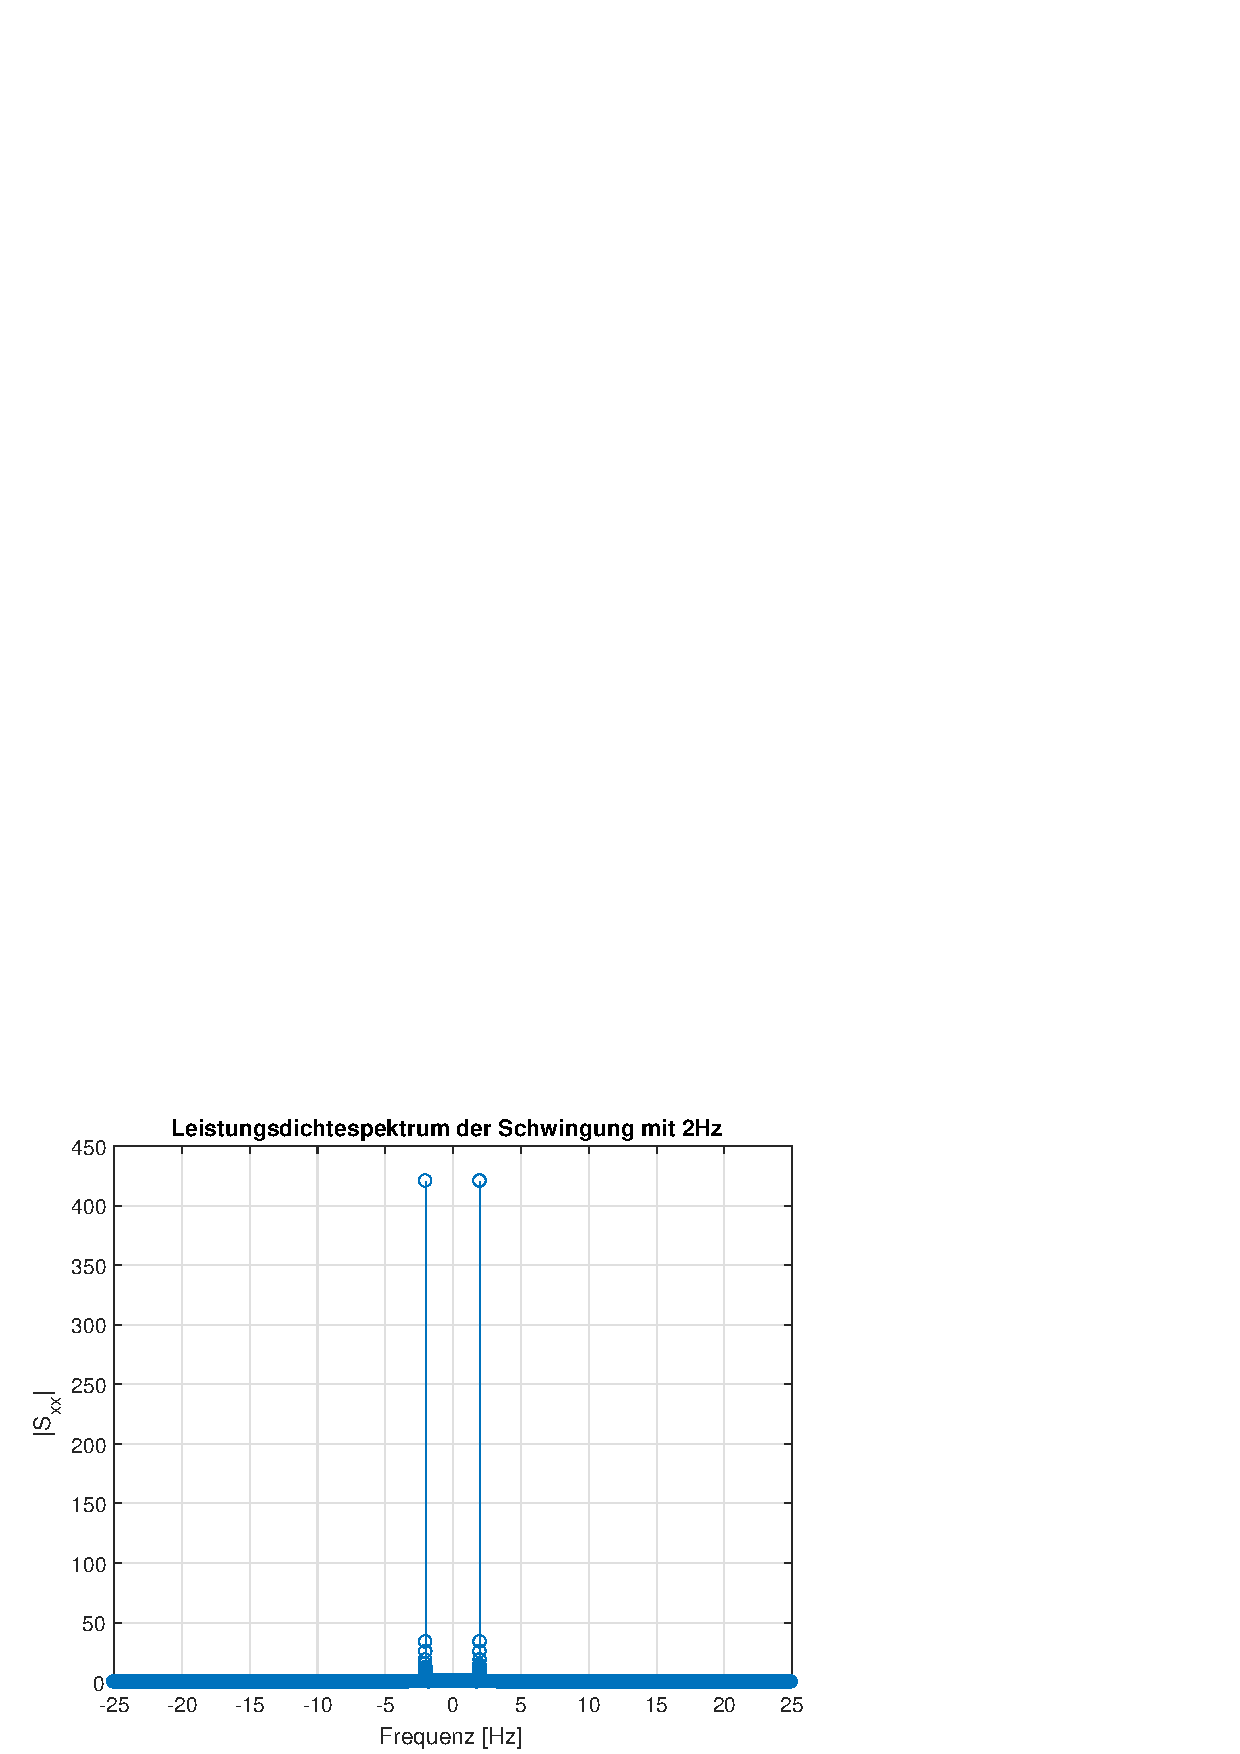
\includegraphics[width=0.5\linewidth]{img/lds_sinefreq_2}
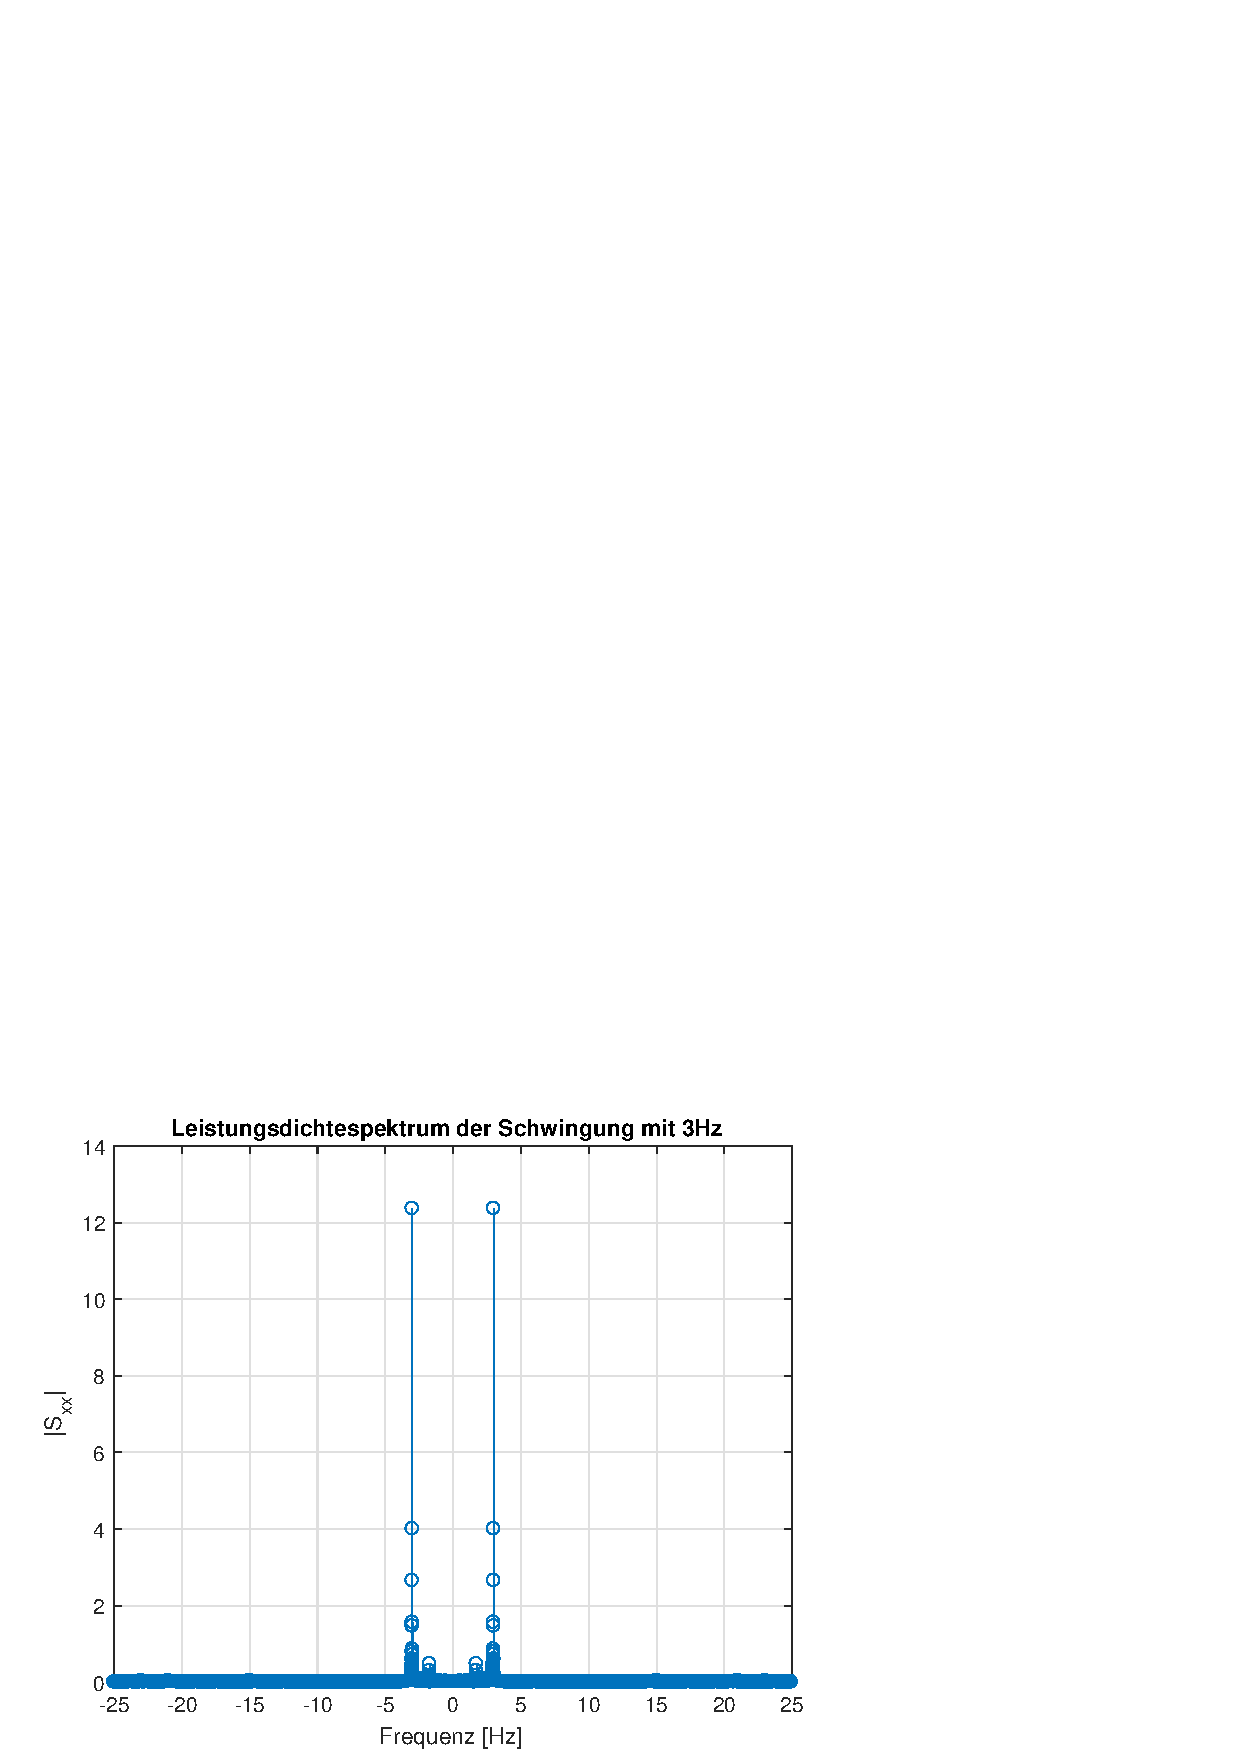
\includegraphics[width=0.5\linewidth]{img/lds_sinefreq_3}
\end{figure}
\begin{figure}[h!]
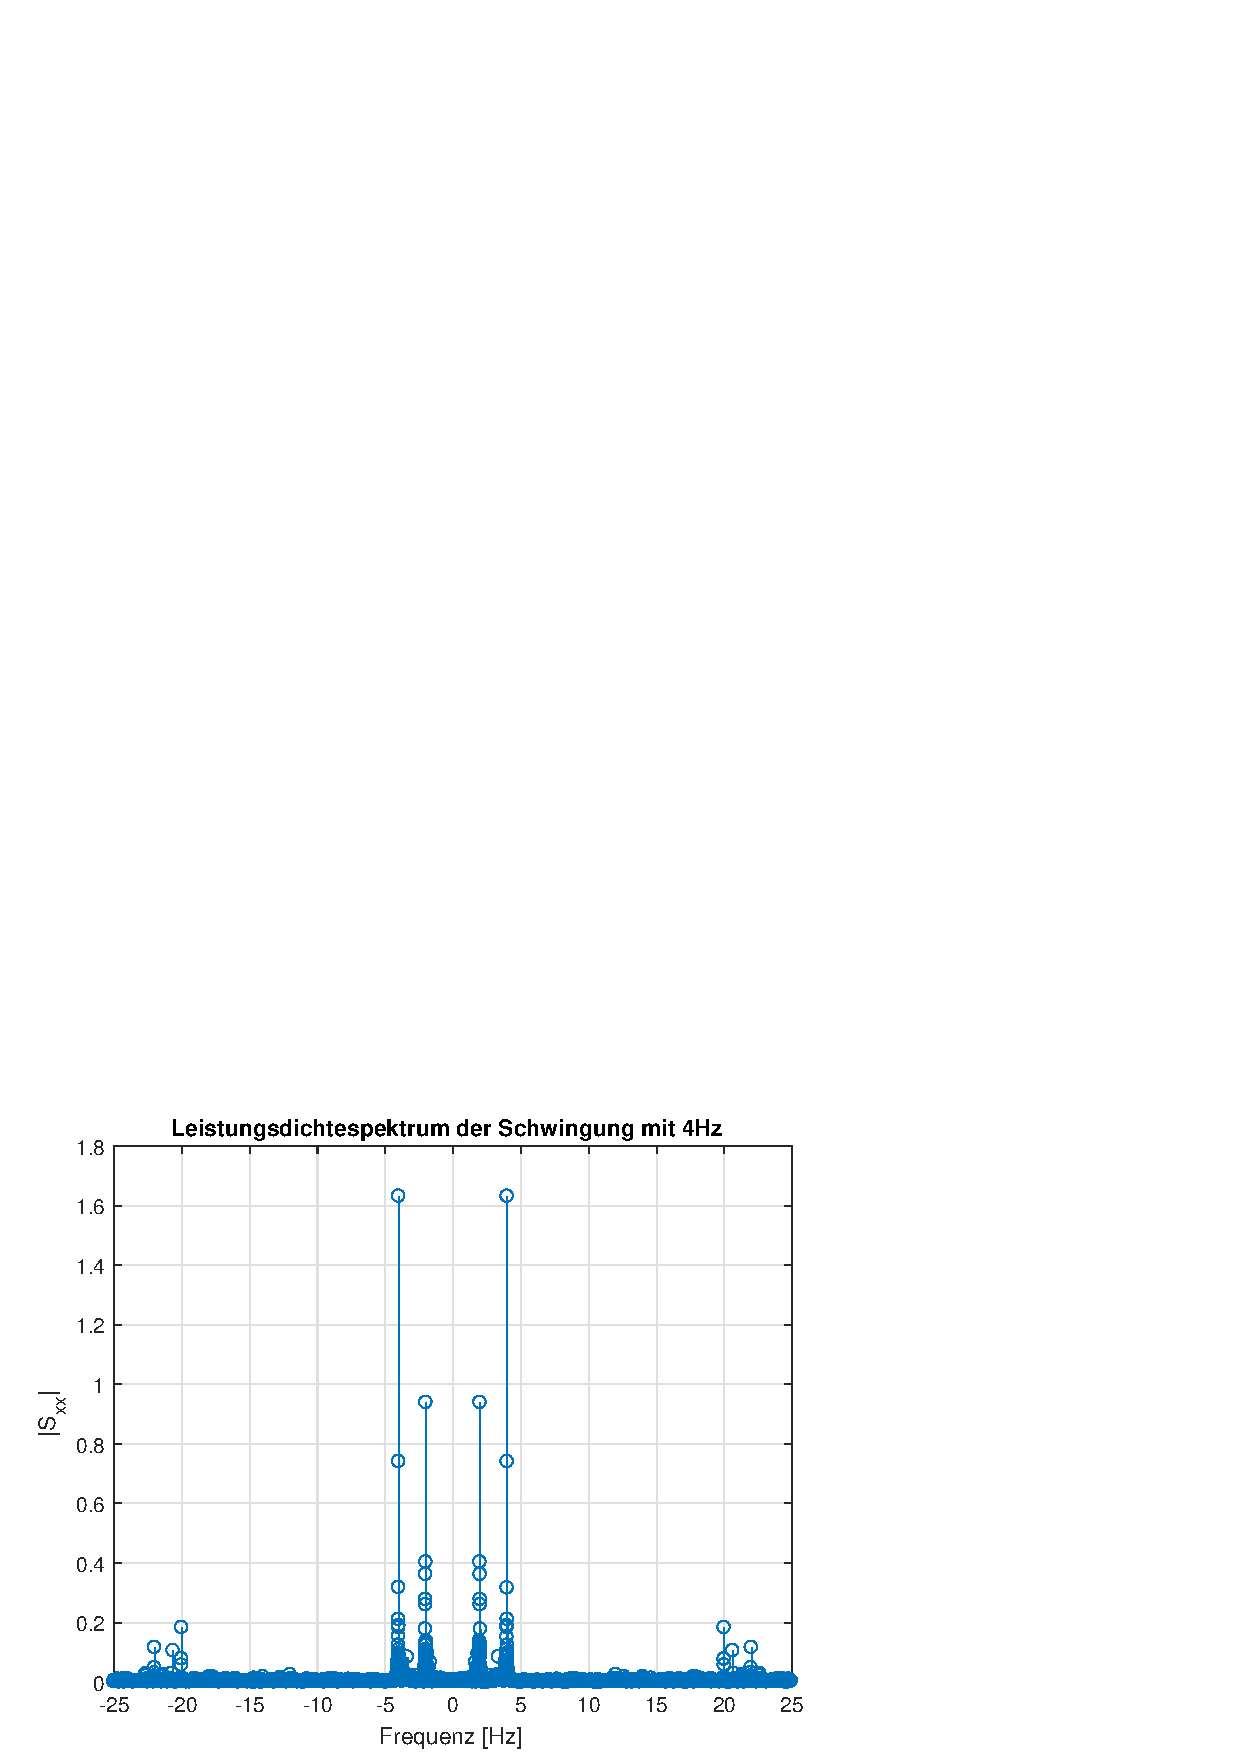
\includegraphics[width=0.5\linewidth]{img/lds_sinefreq_4}
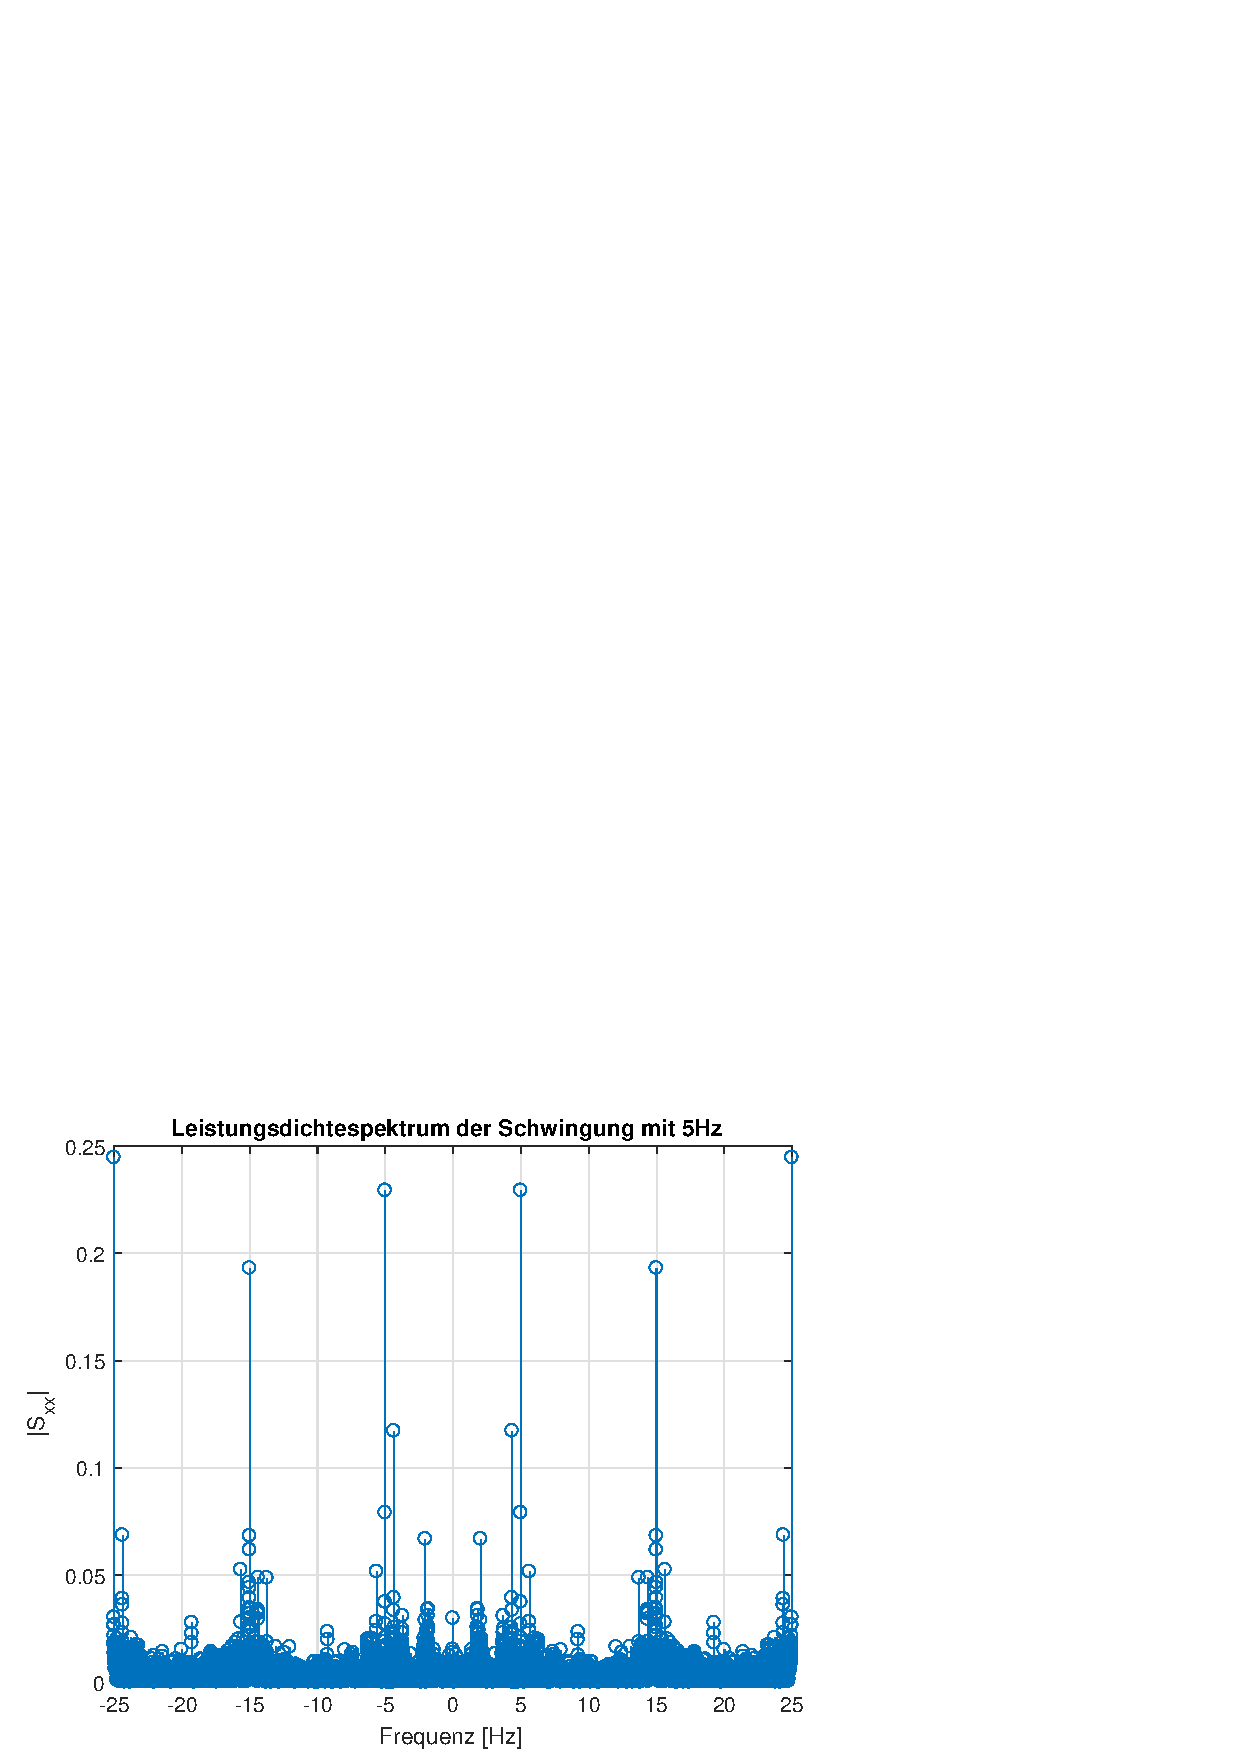
\includegraphics[width=0.5\linewidth]{img/lds_sinefreq_5}
\end{figure}
\newpage
\begin{figure}[h!]
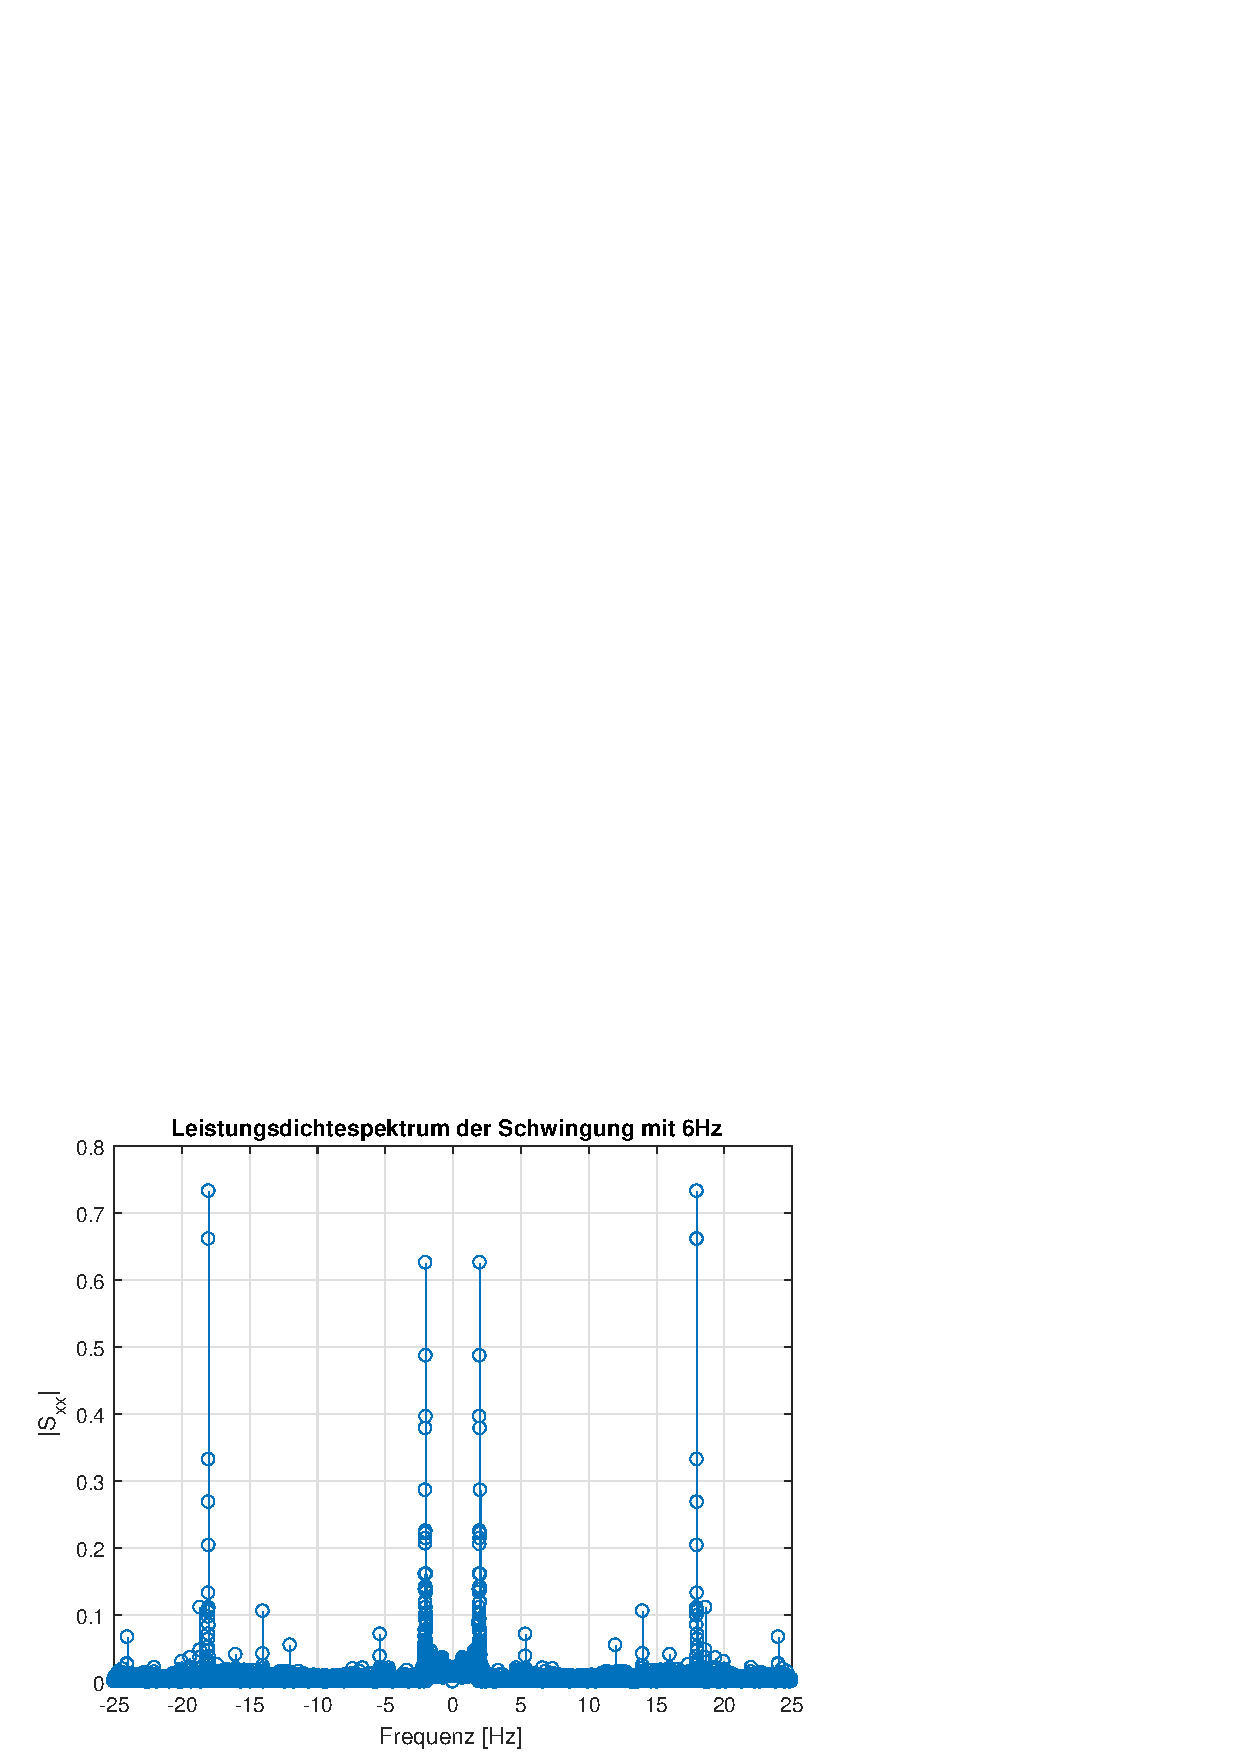
\includegraphics[width=0.5\linewidth]{img/lds_sinefreq_6}
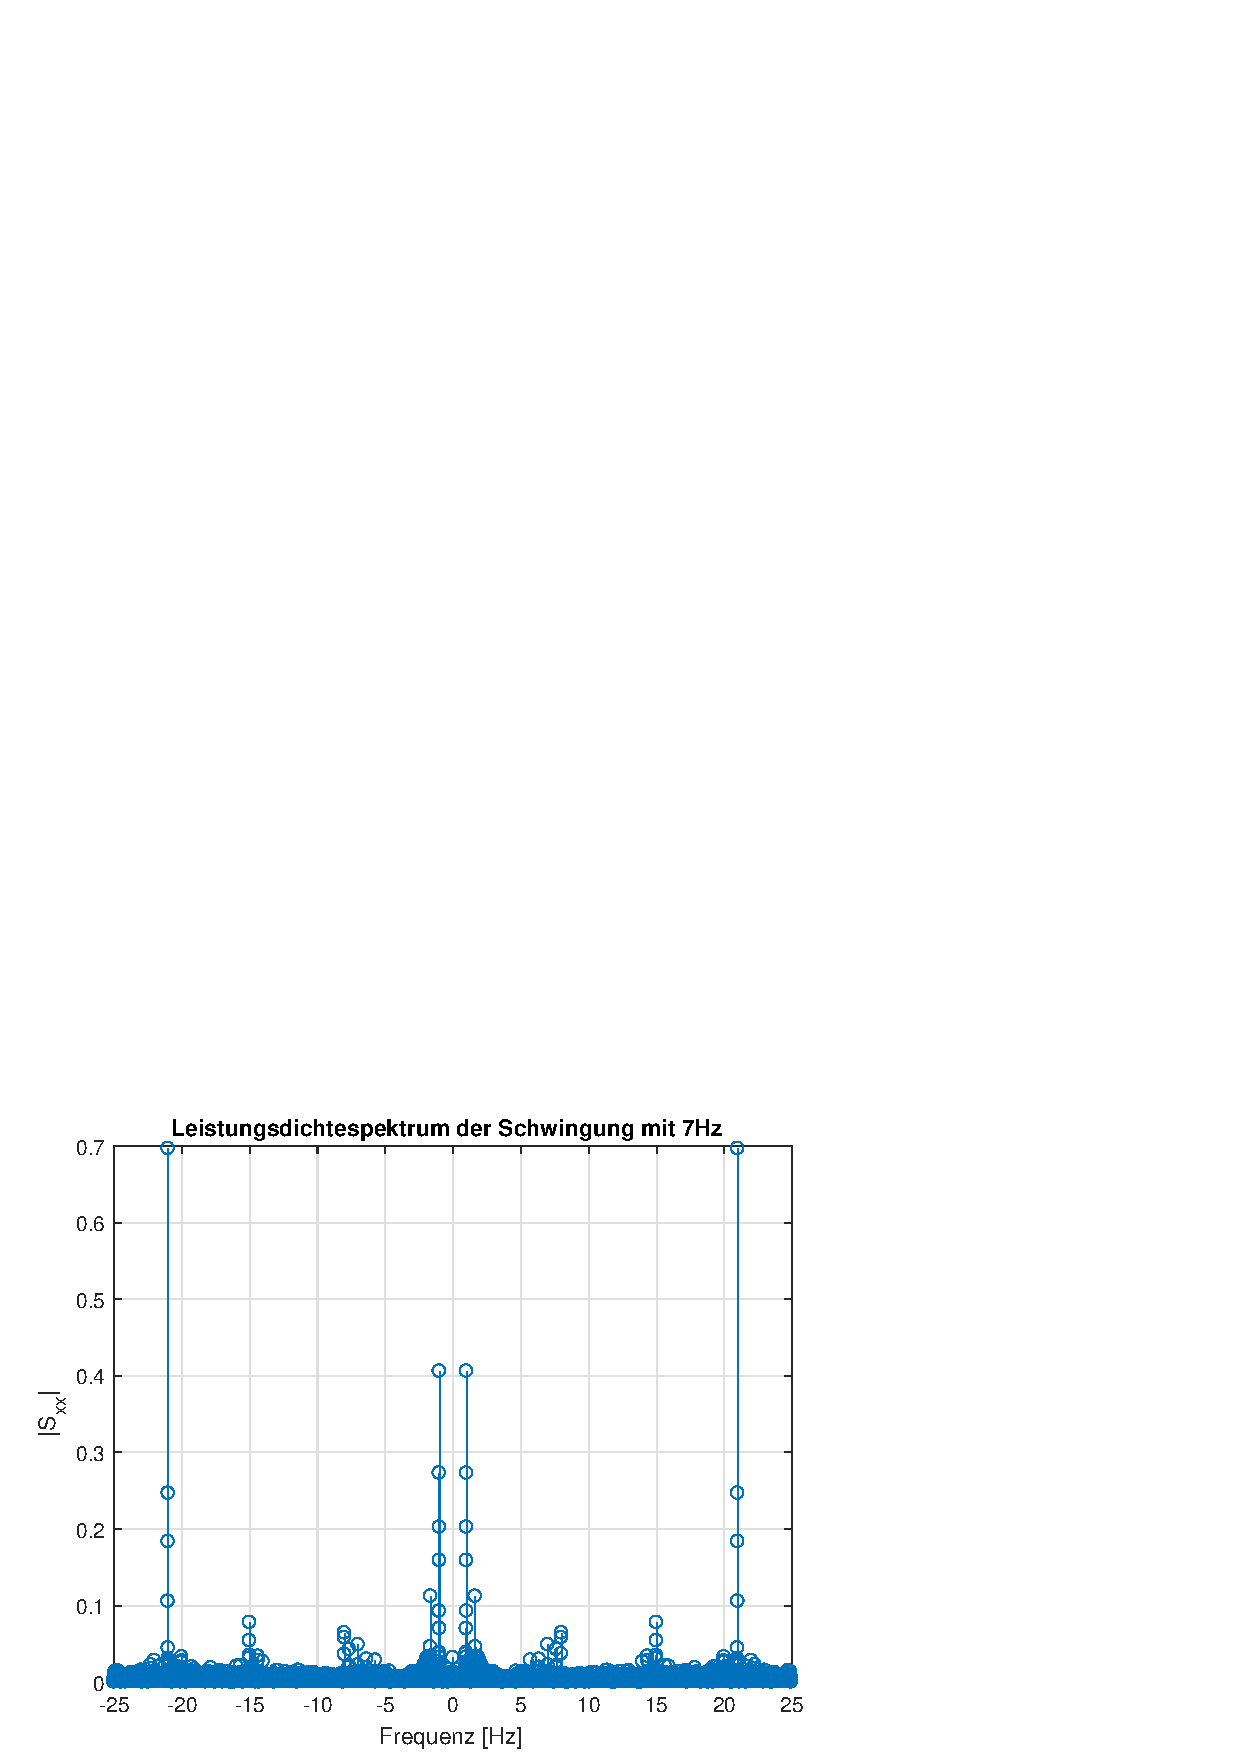
\includegraphics[width=0.5\linewidth]{img/lds_sinefreq_7}
\end{figure}
\begin{figure}[h!]
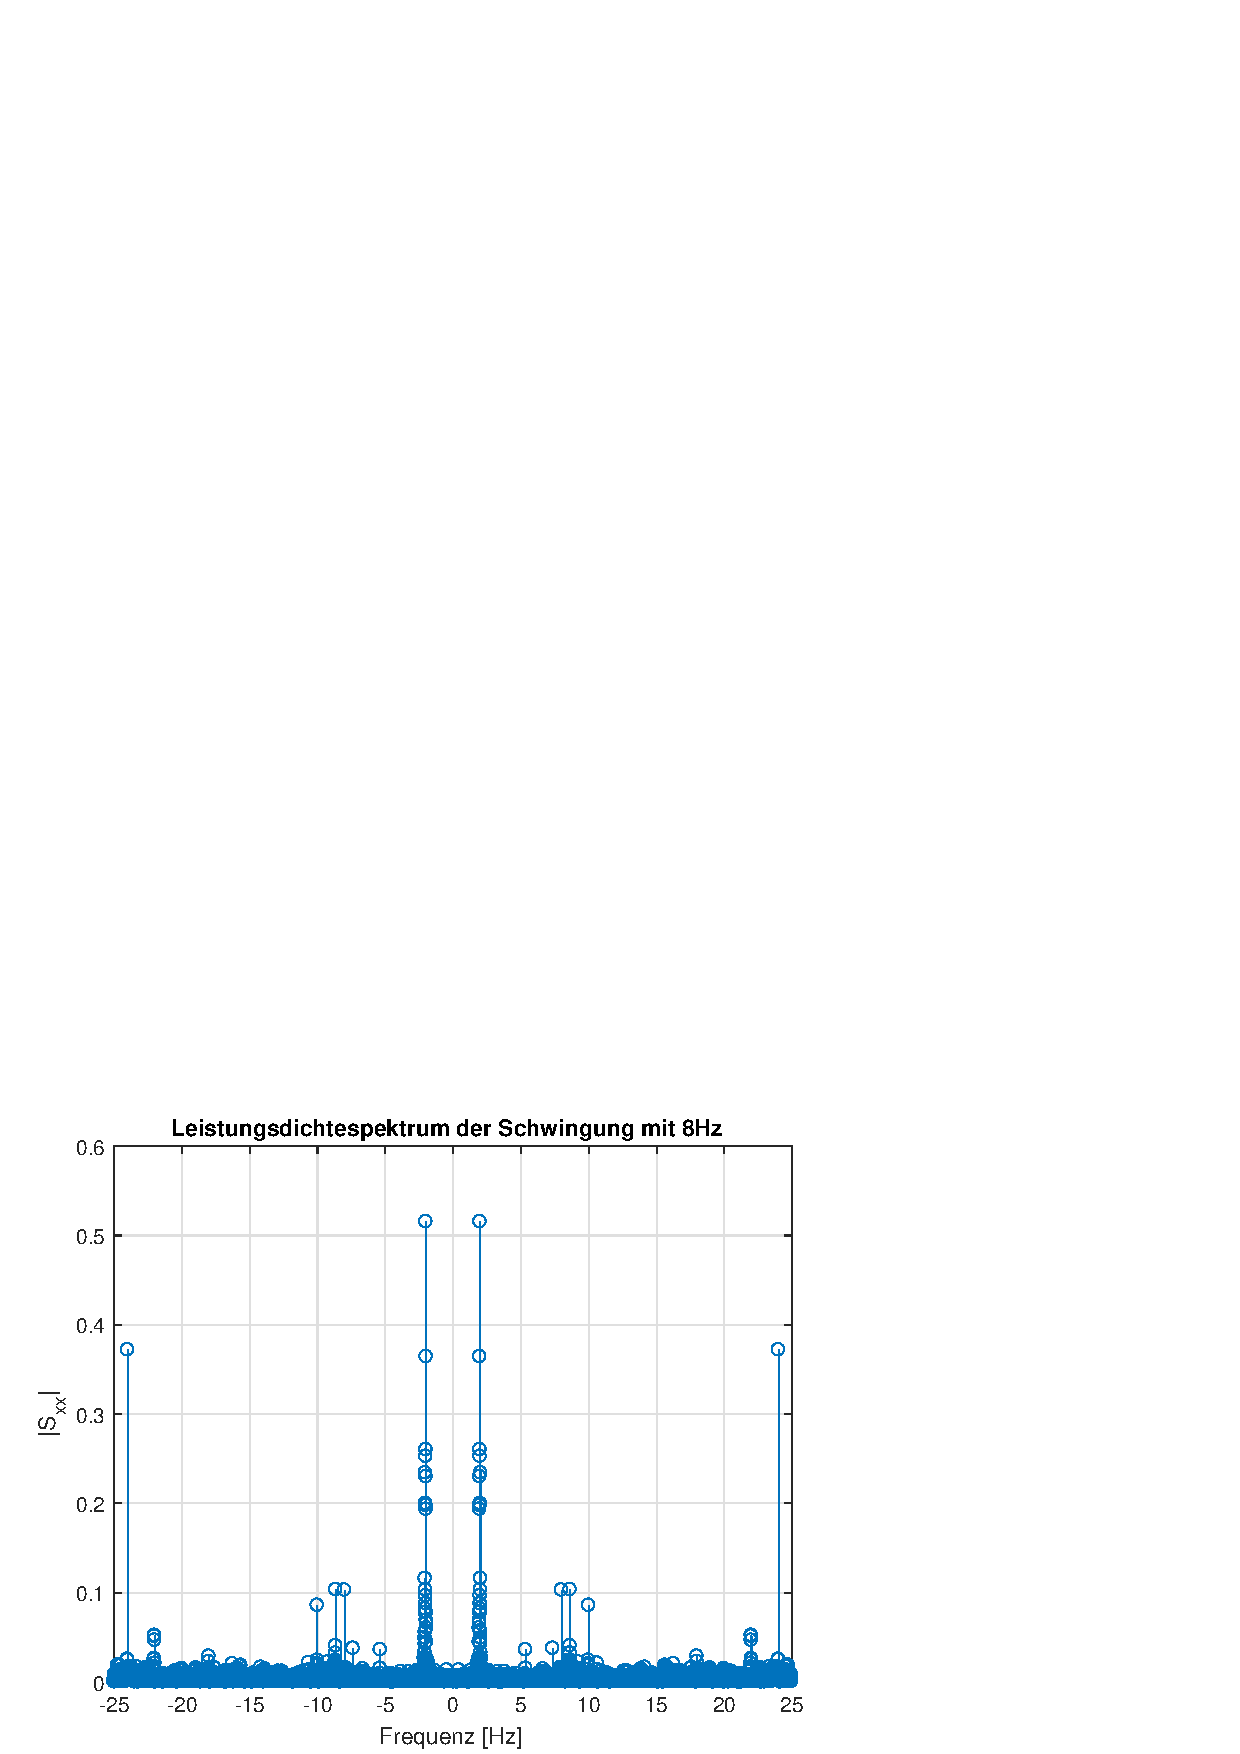
\includegraphics[width=0.5\linewidth]{img/lds_sinefreq_8}
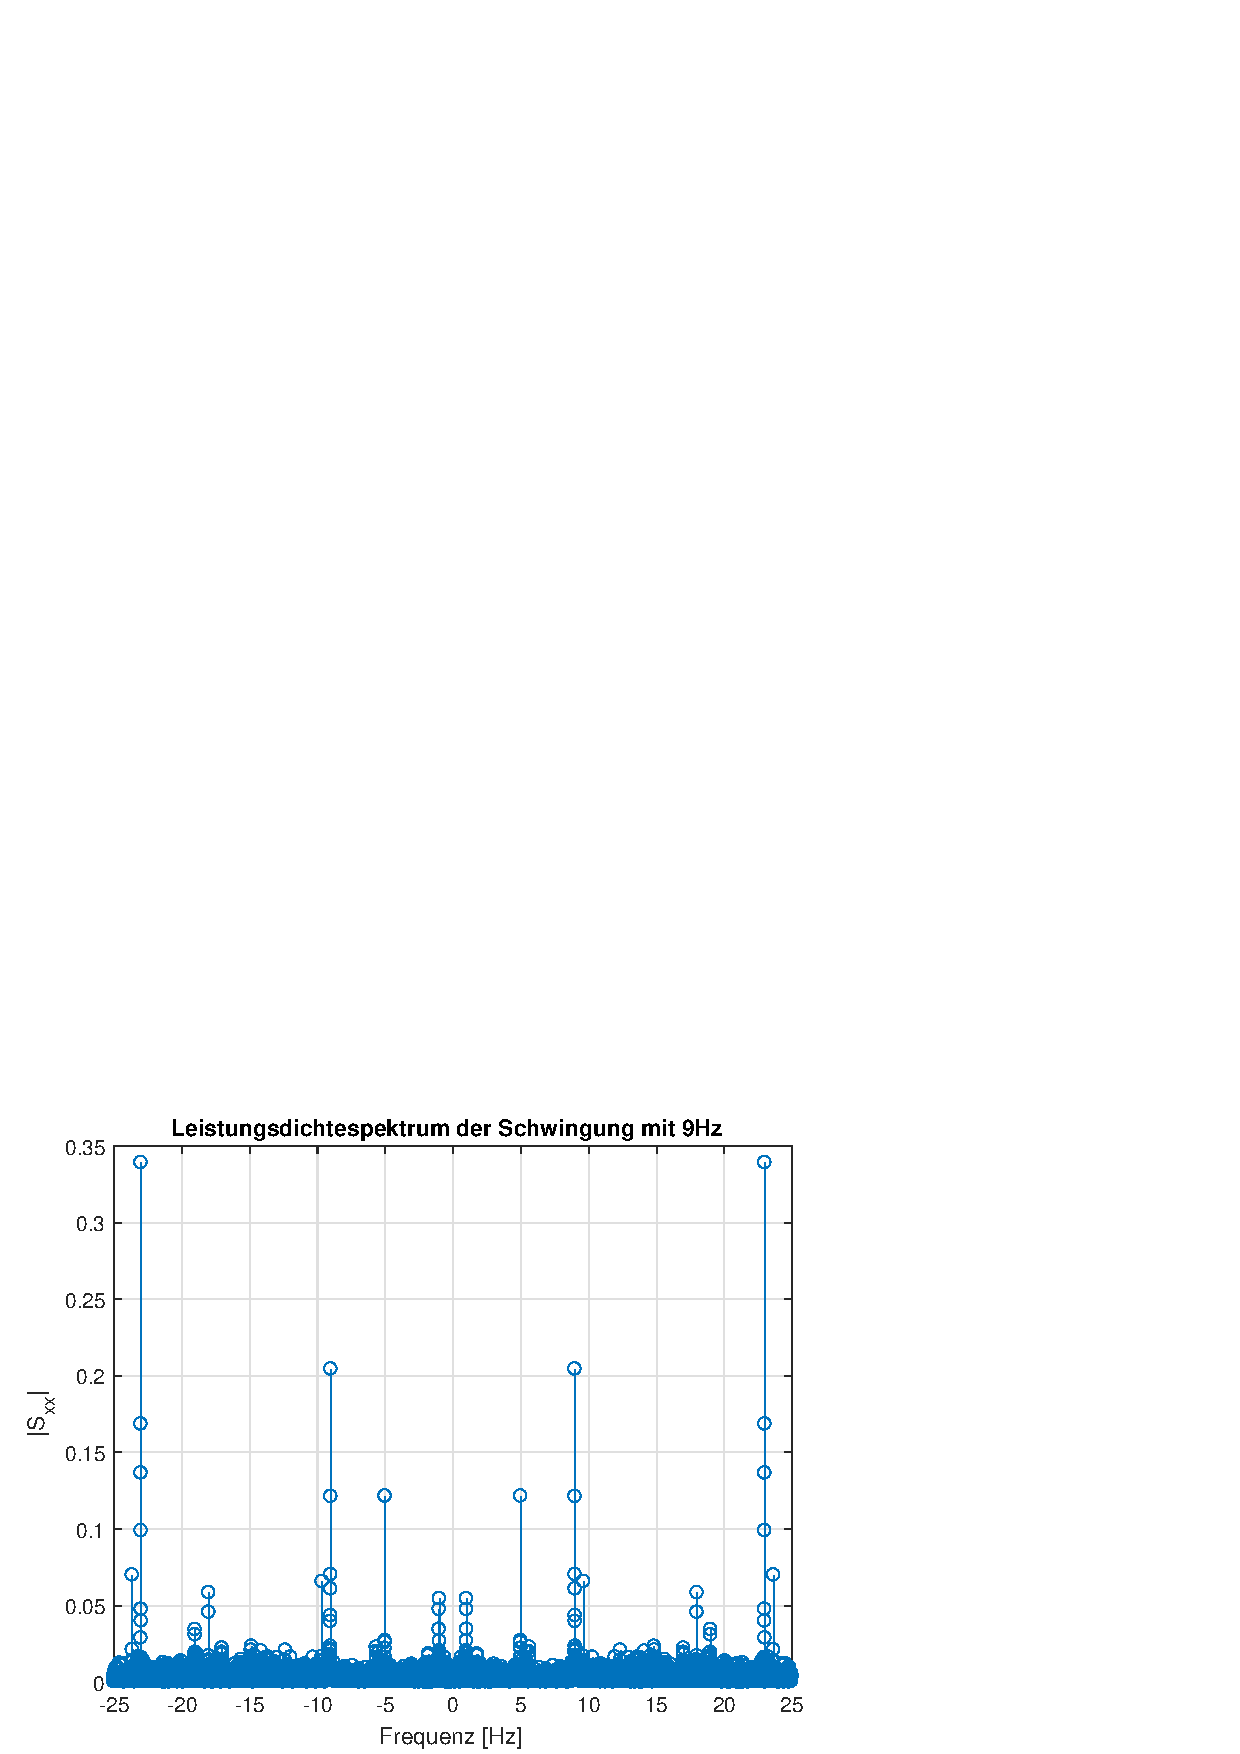
\includegraphics[width=0.5\linewidth]{img/lds_sinefreq_9}
\end{figure}
\begin{figure}[h!]
\centering
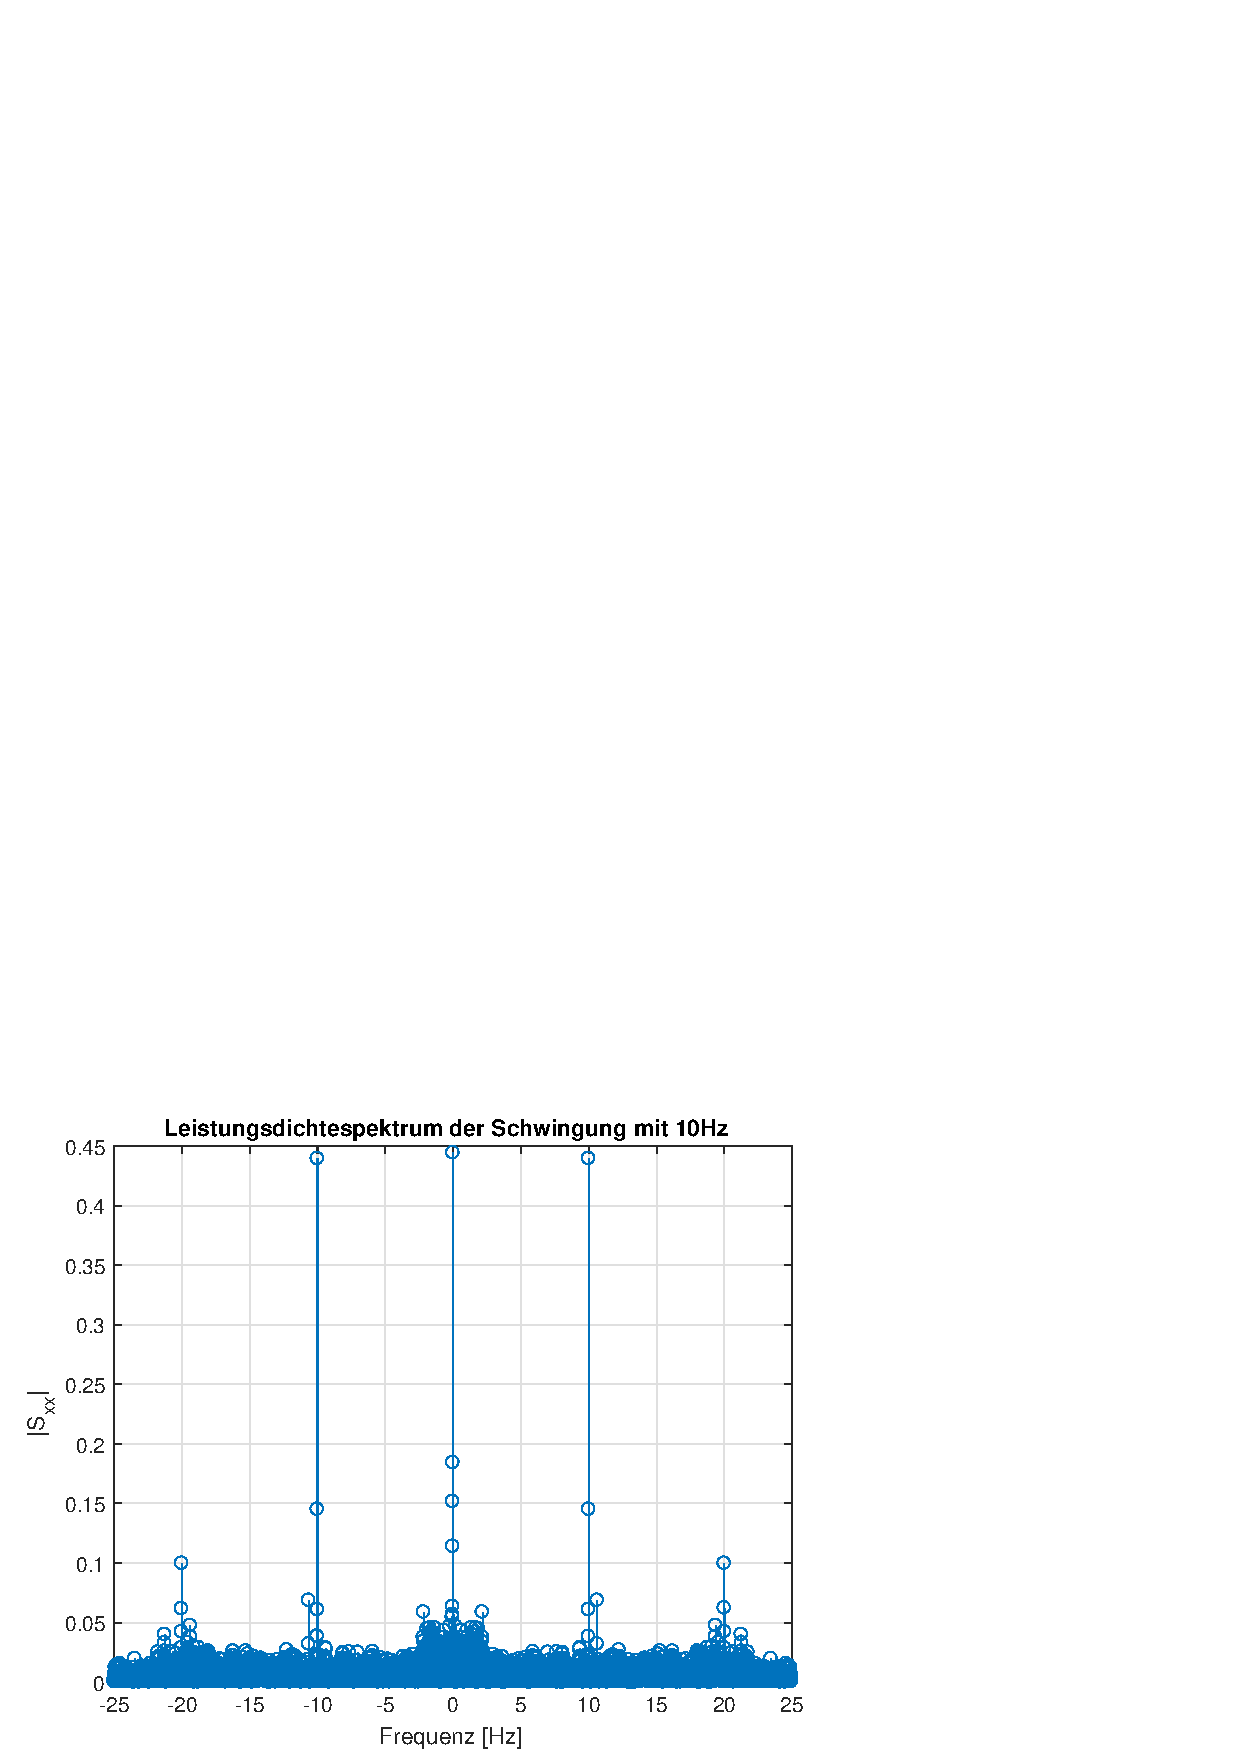
\includegraphics[width=0.5\linewidth]{img/lds_sinefreq_10}
\end{figure}


\newpage
\section{Spektren von $\varphi$ aus Gyro-Integration bei Sinusanregung}
\subsection{DFT-Spektren von $\varphi$ bei $T_M = sin(2\pi\cdot f\cdot t)$}
\begin{figure}[h!]
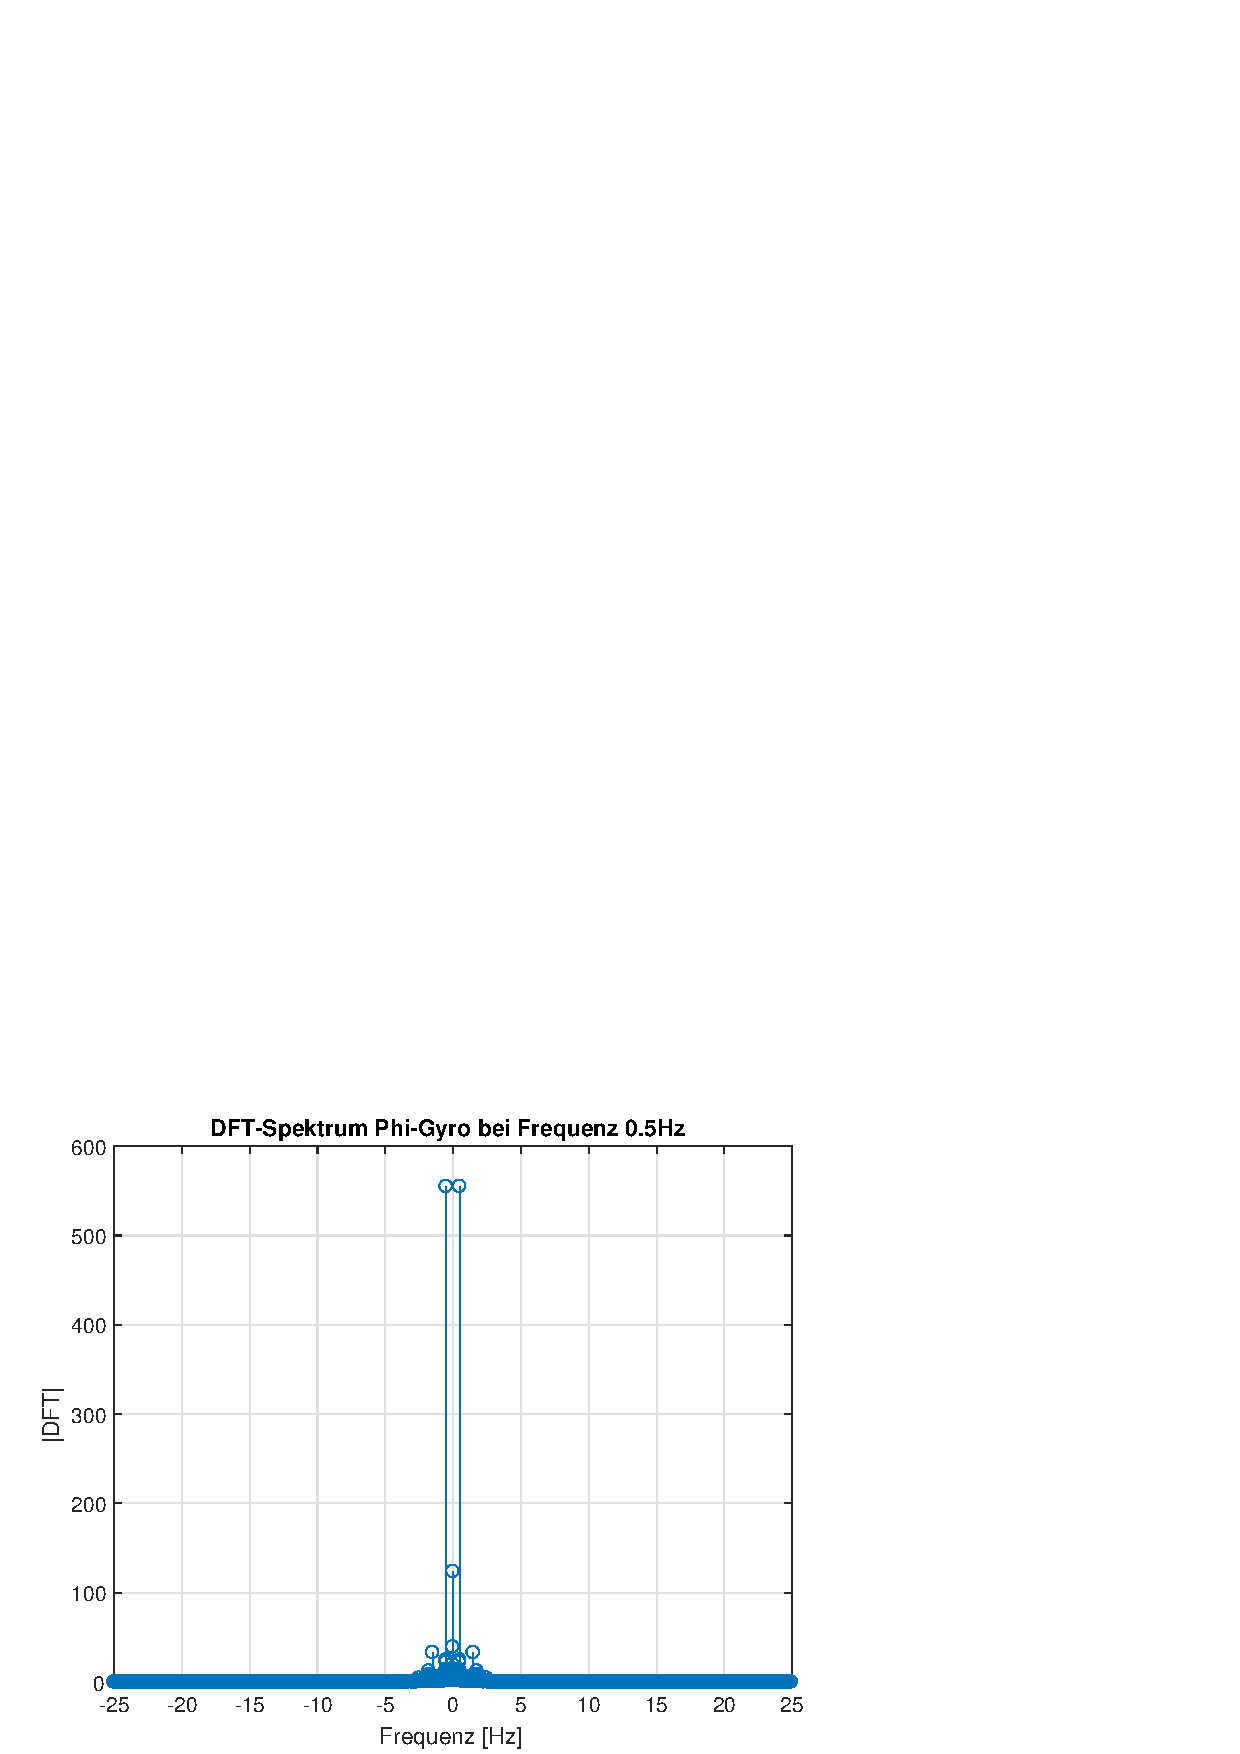
\includegraphics[width=0.5\linewidth]{img/dft_phi_g_1}
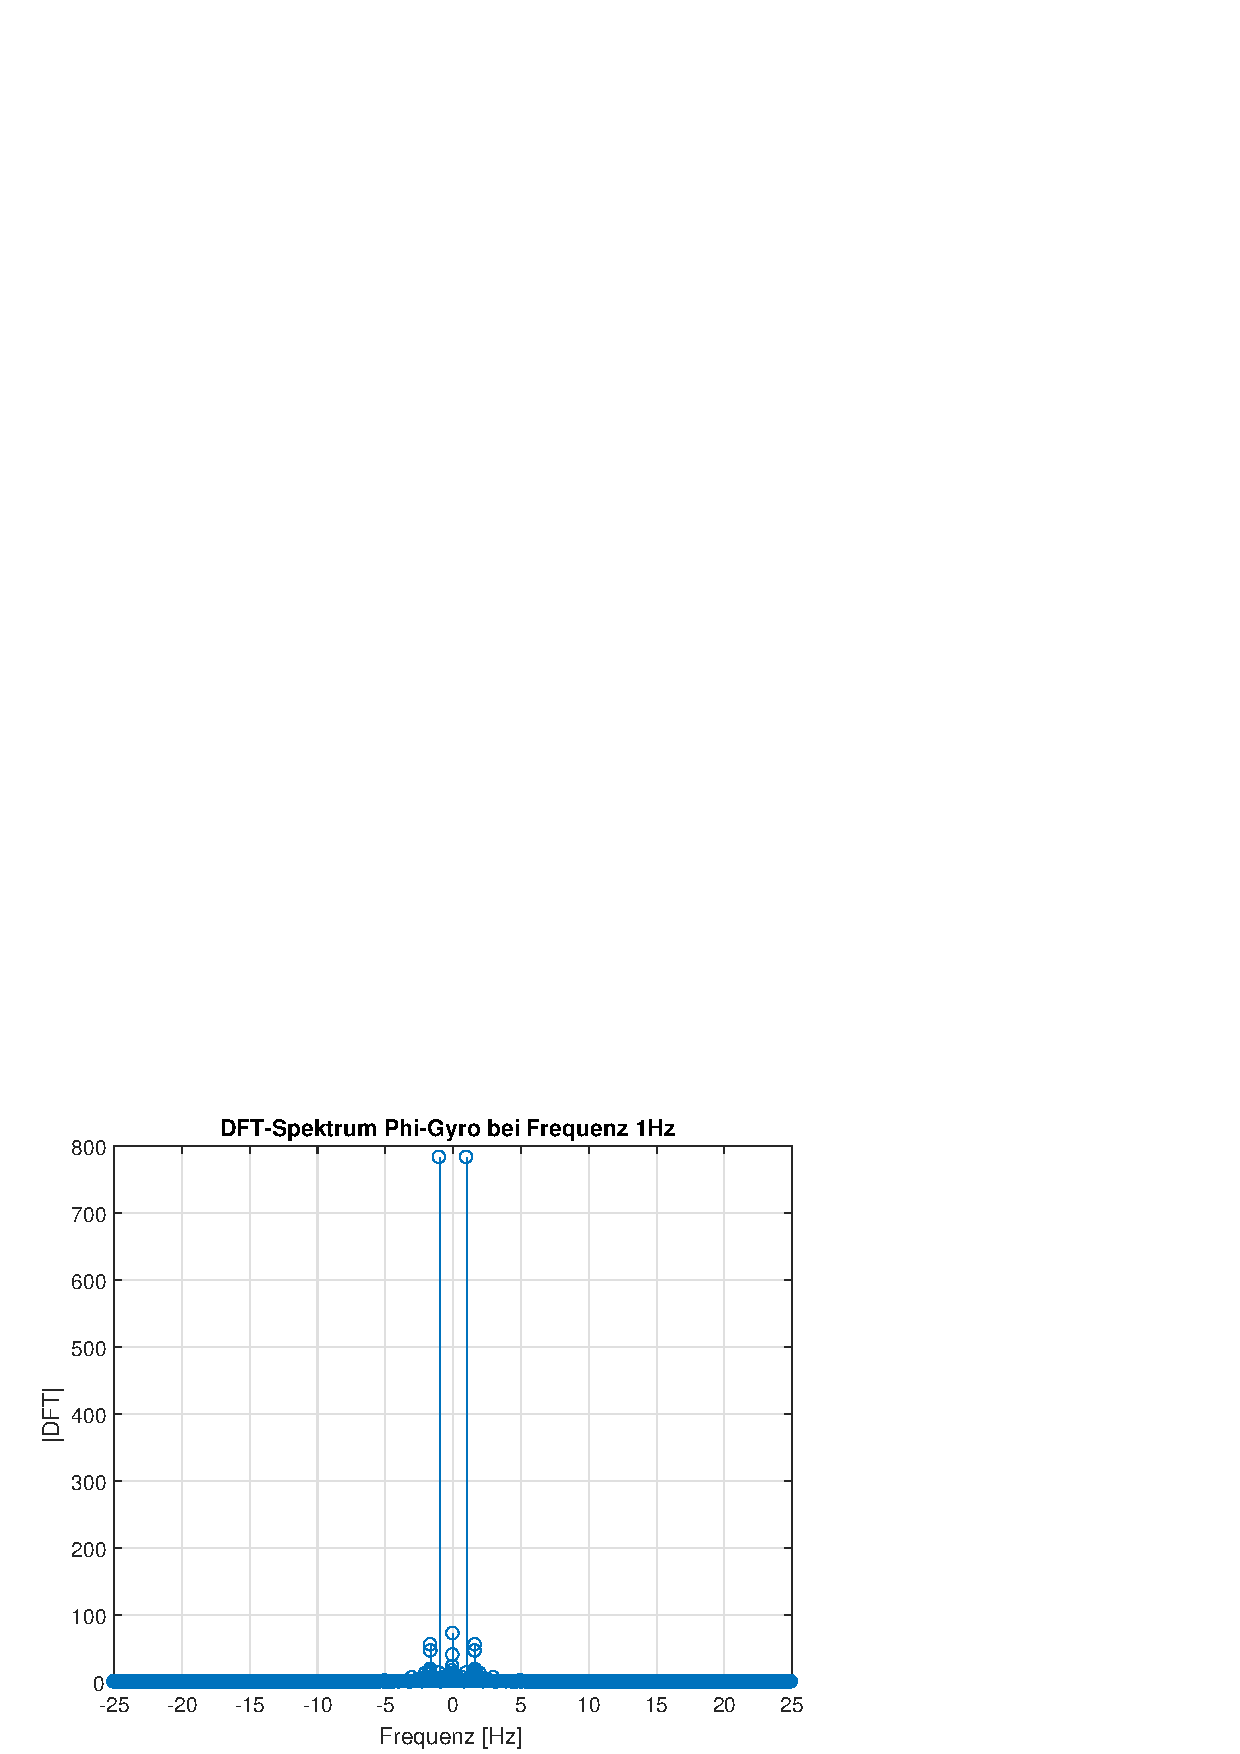
\includegraphics[width=0.5\linewidth]{img/dft_phi_g_2}
\end{figure}
\begin{figure}[h!]
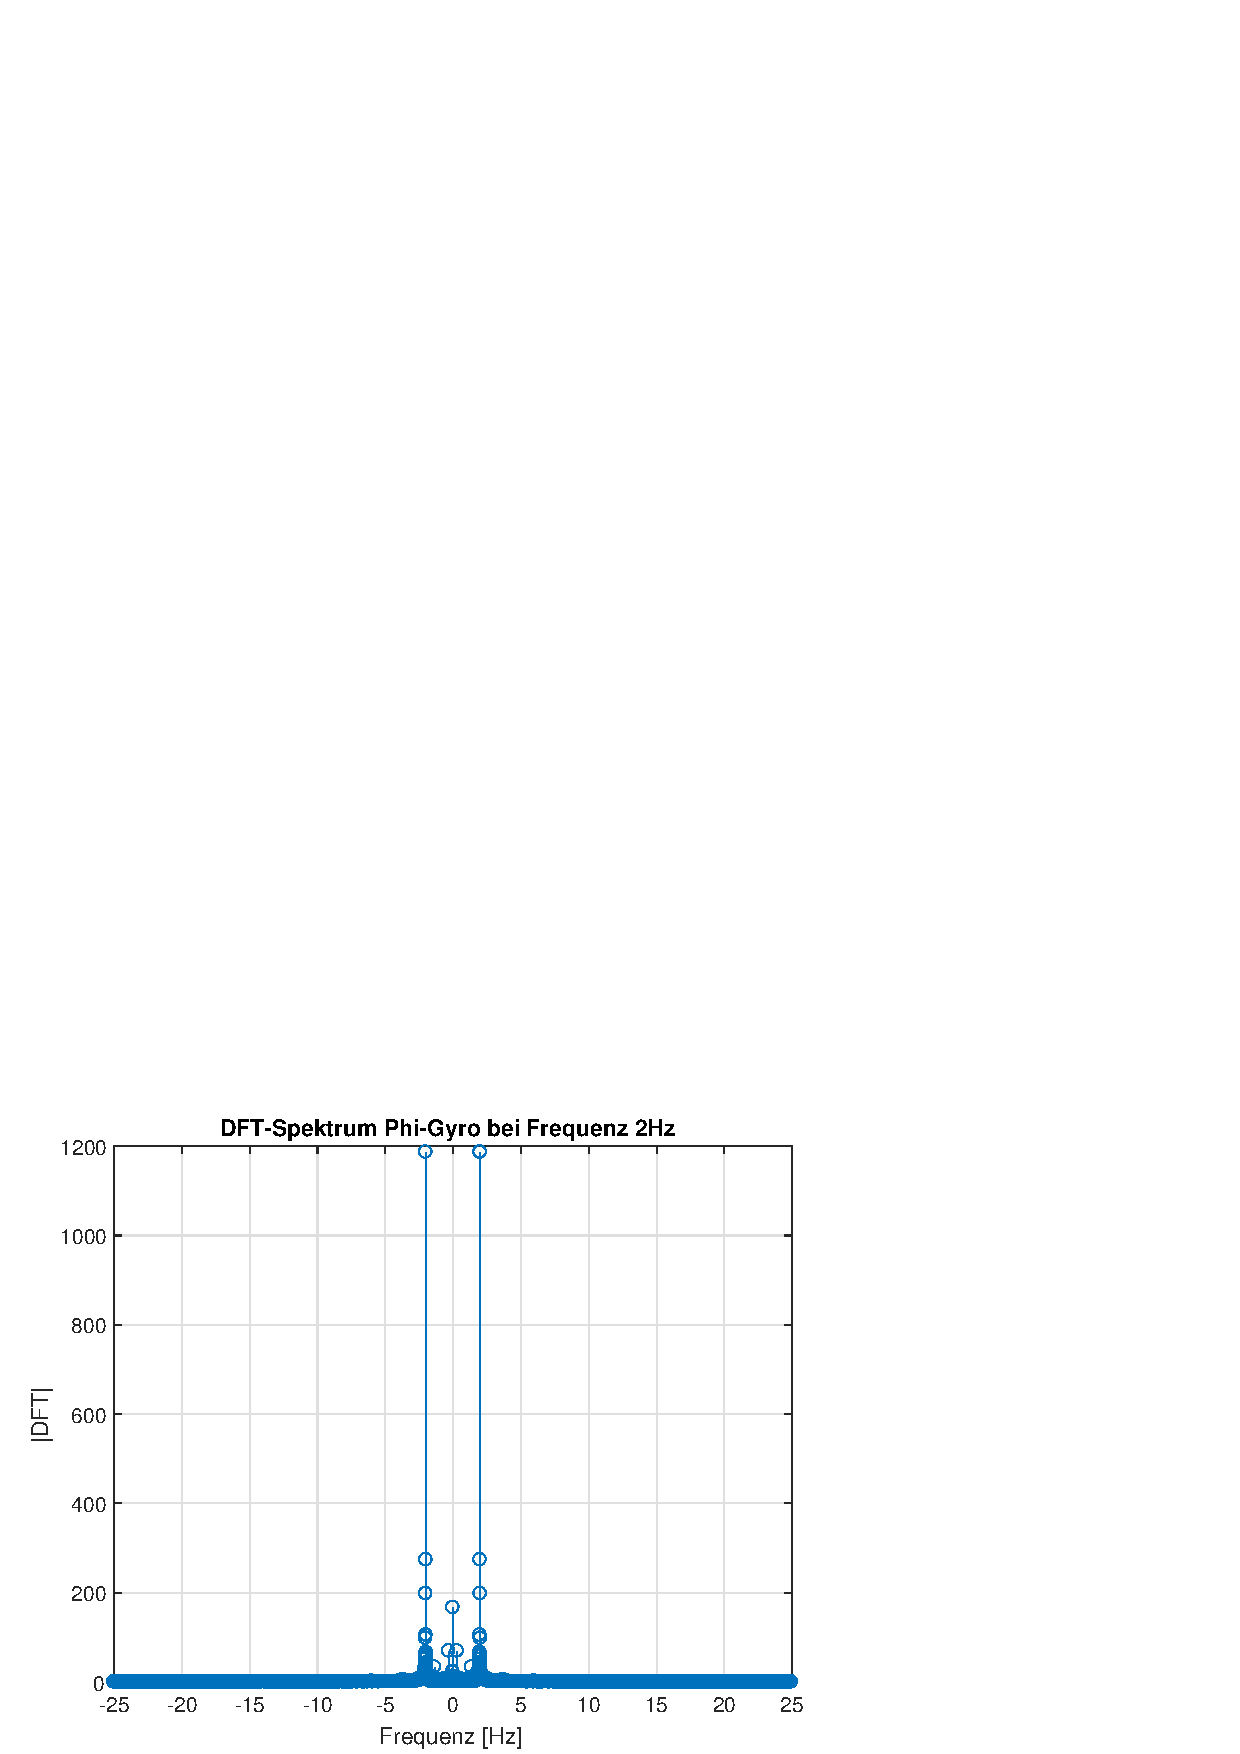
\includegraphics[width=0.5\linewidth]{img/dft_phi_g_3}
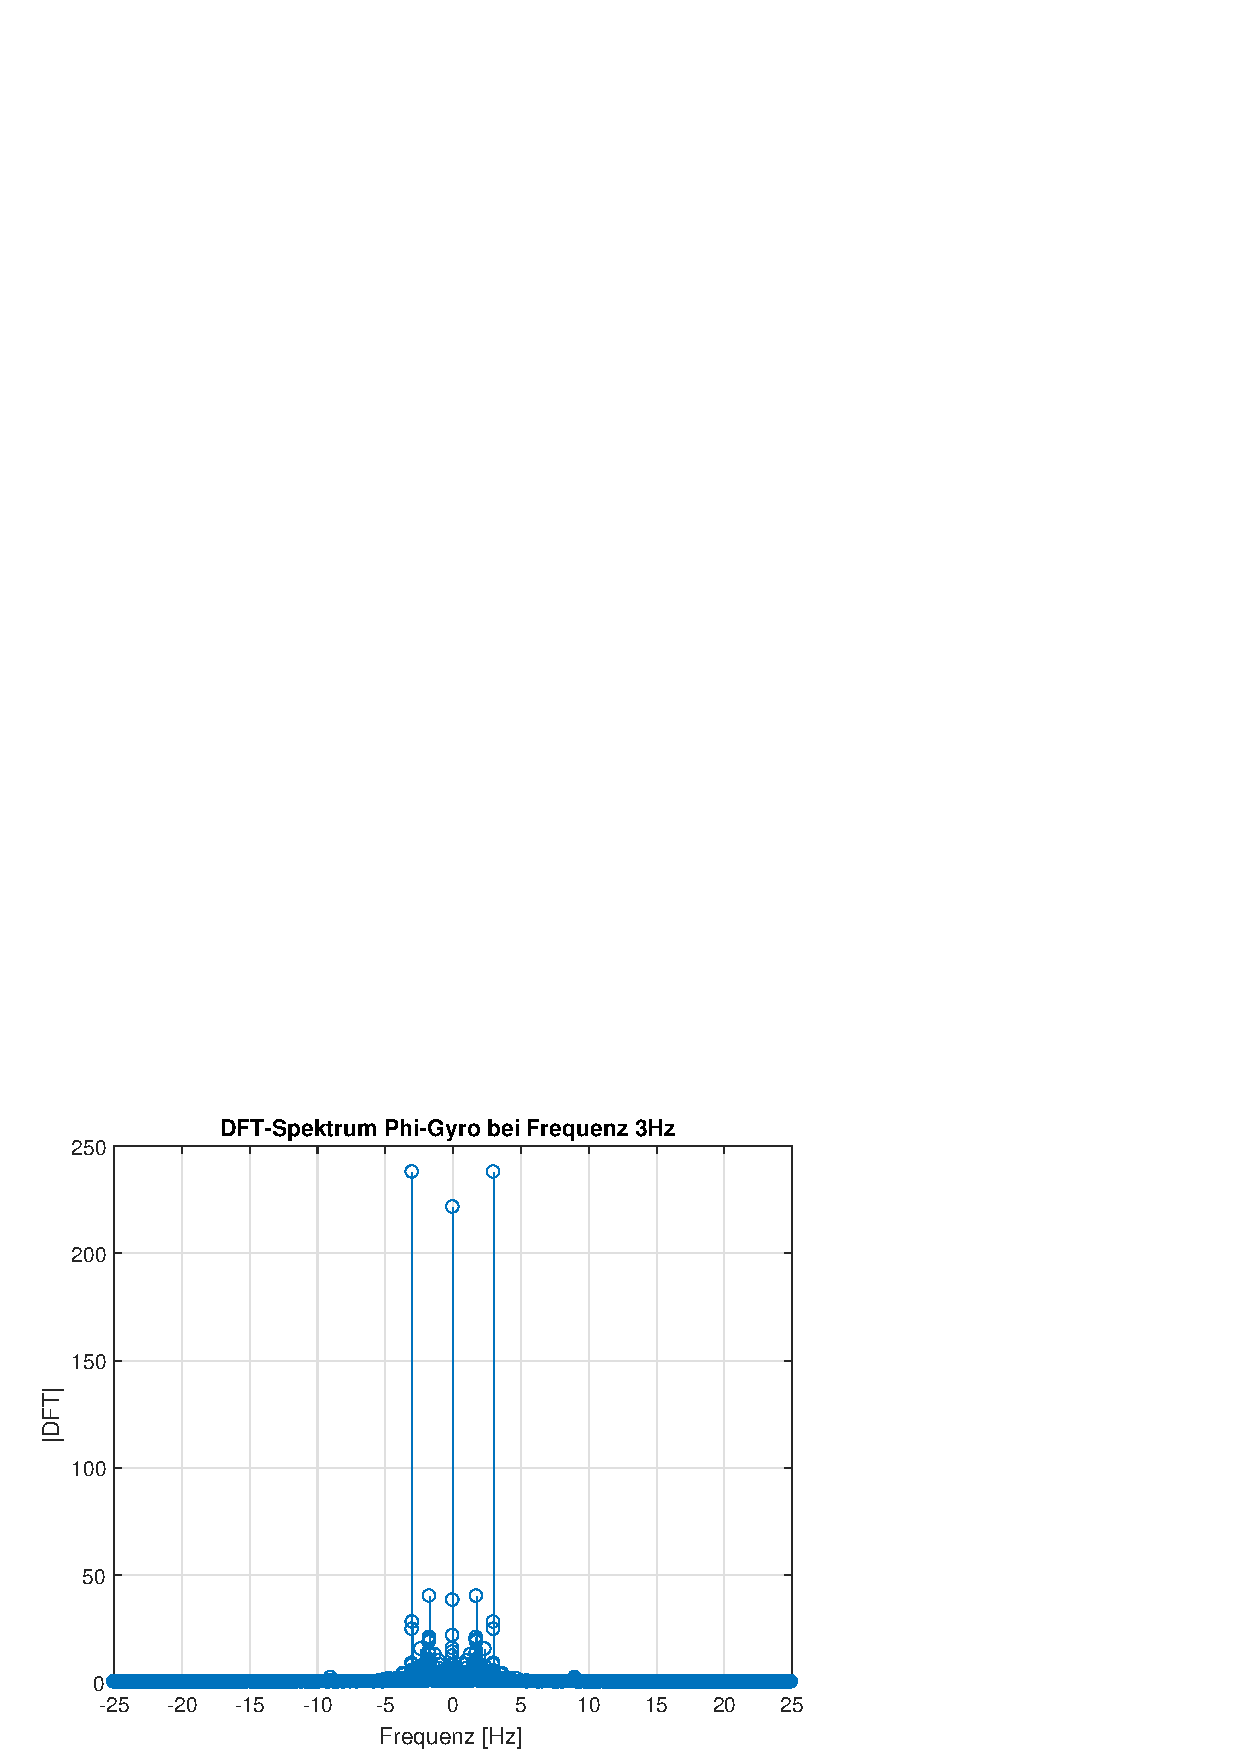
\includegraphics[width=0.5\linewidth]{img/dft_phi_g_4}
\end{figure}
\begin{figure}[h!]
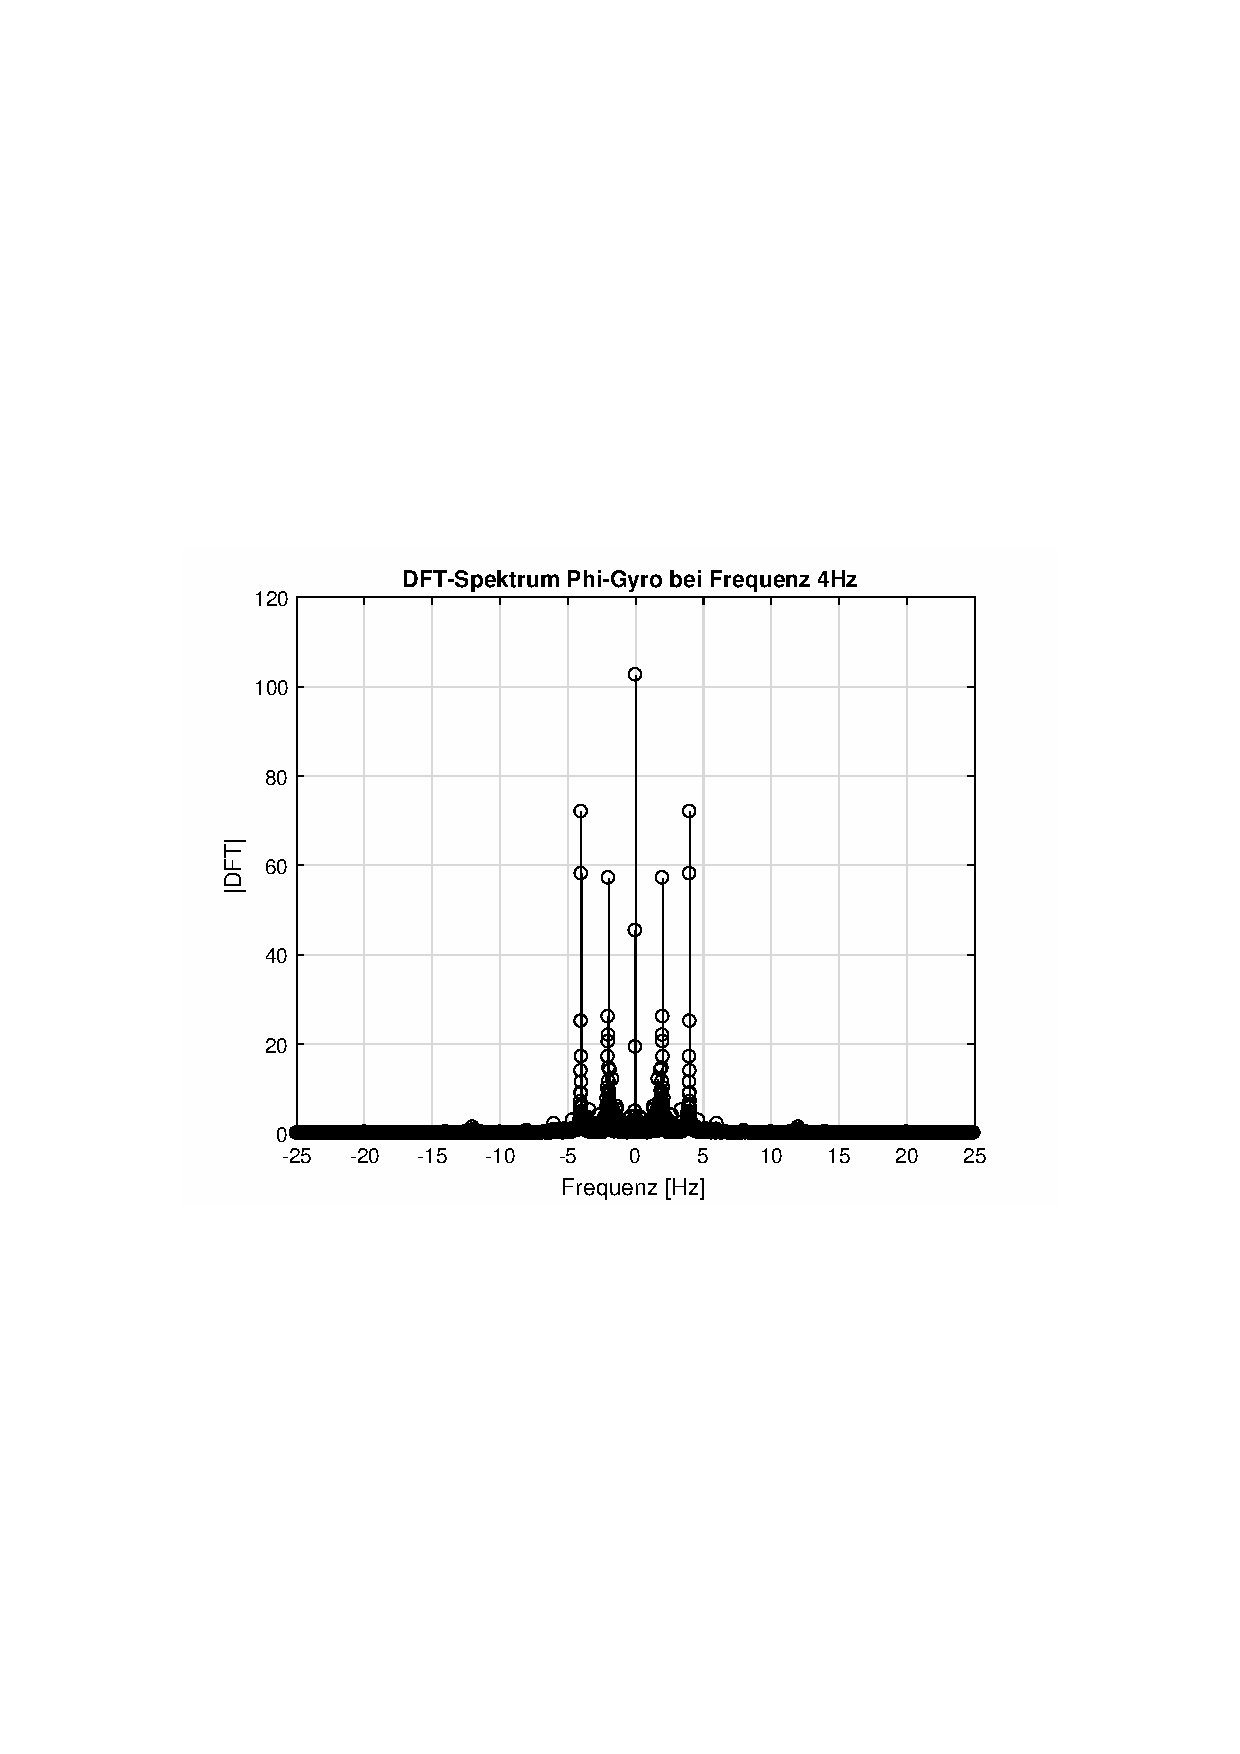
\includegraphics[width=0.5\linewidth]{img/dft_phi_g_5}
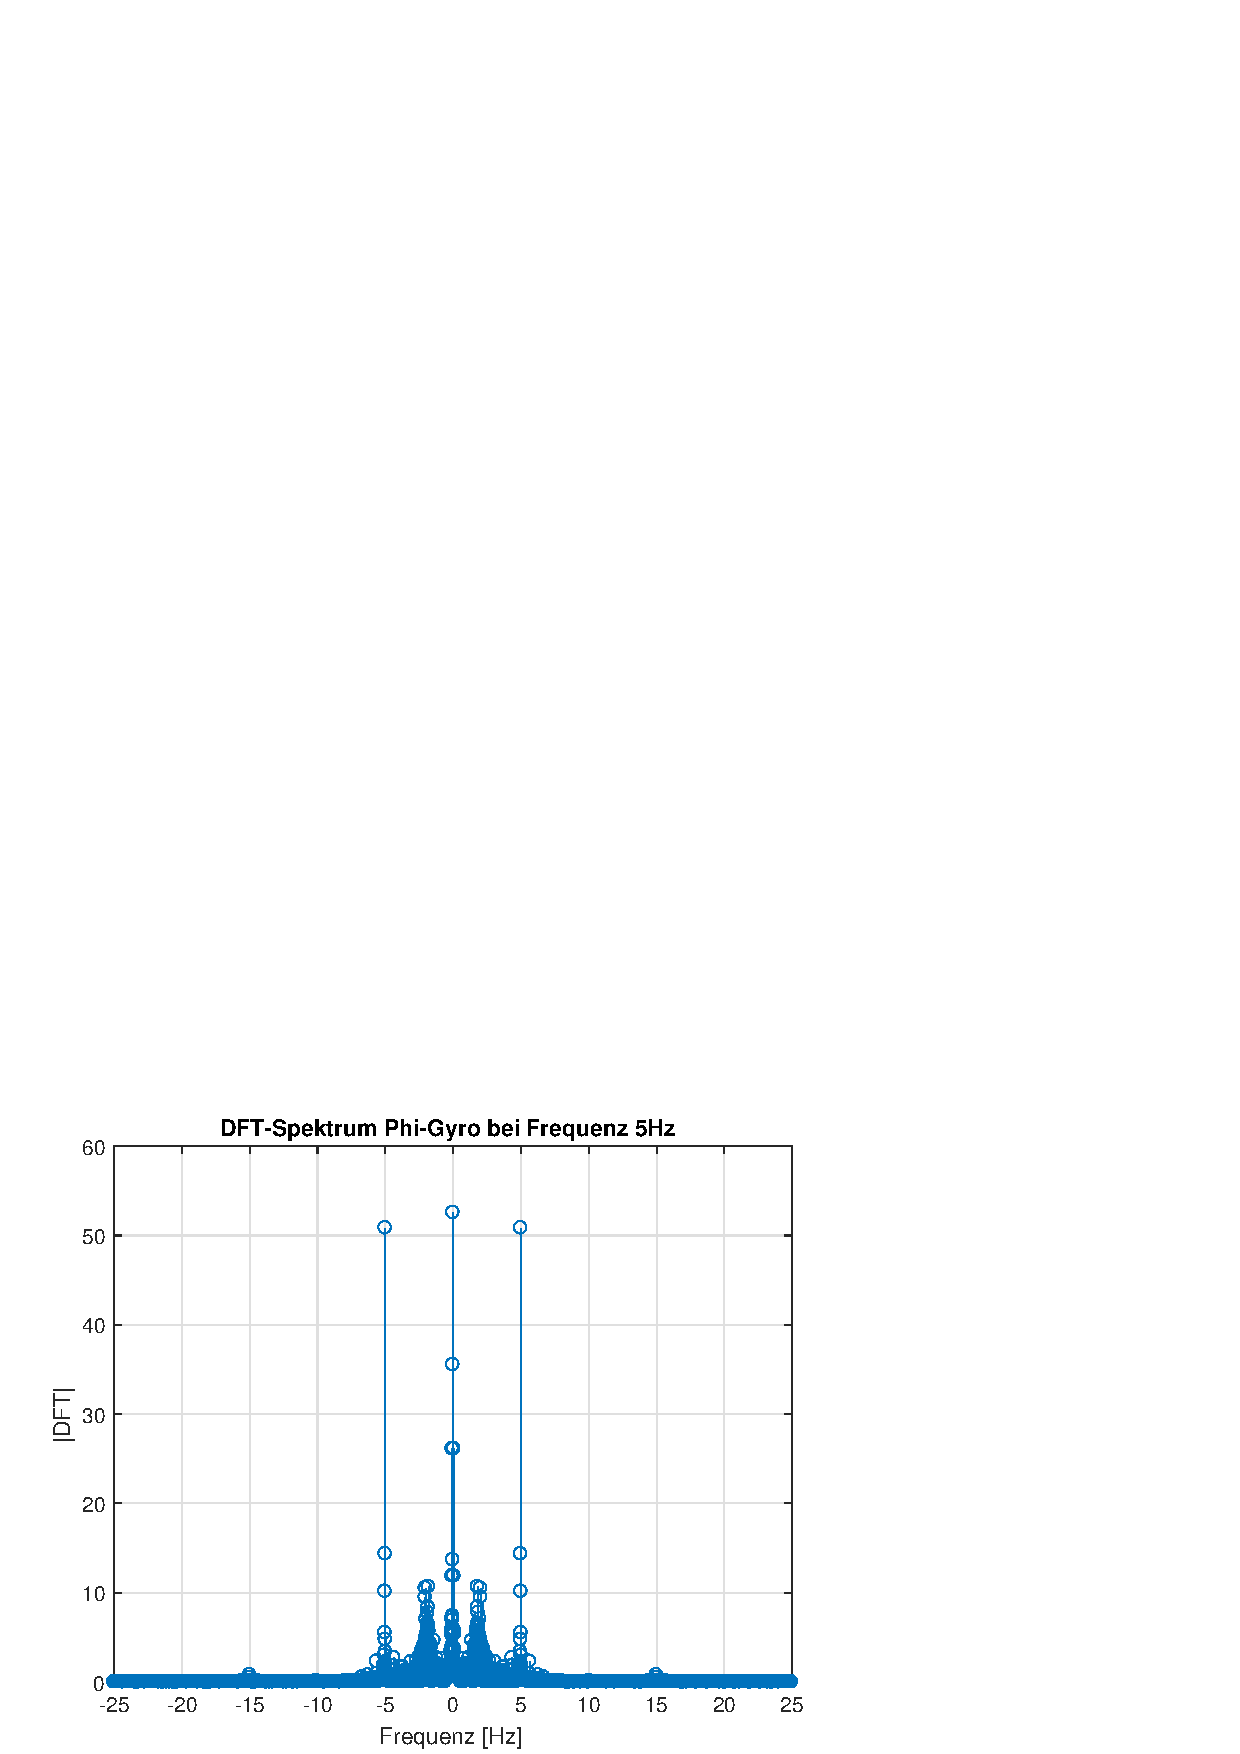
\includegraphics[width=0.5\linewidth]{img/dft_phi_g_6}
\end{figure}
\newpage
\begin{figure}[h!]
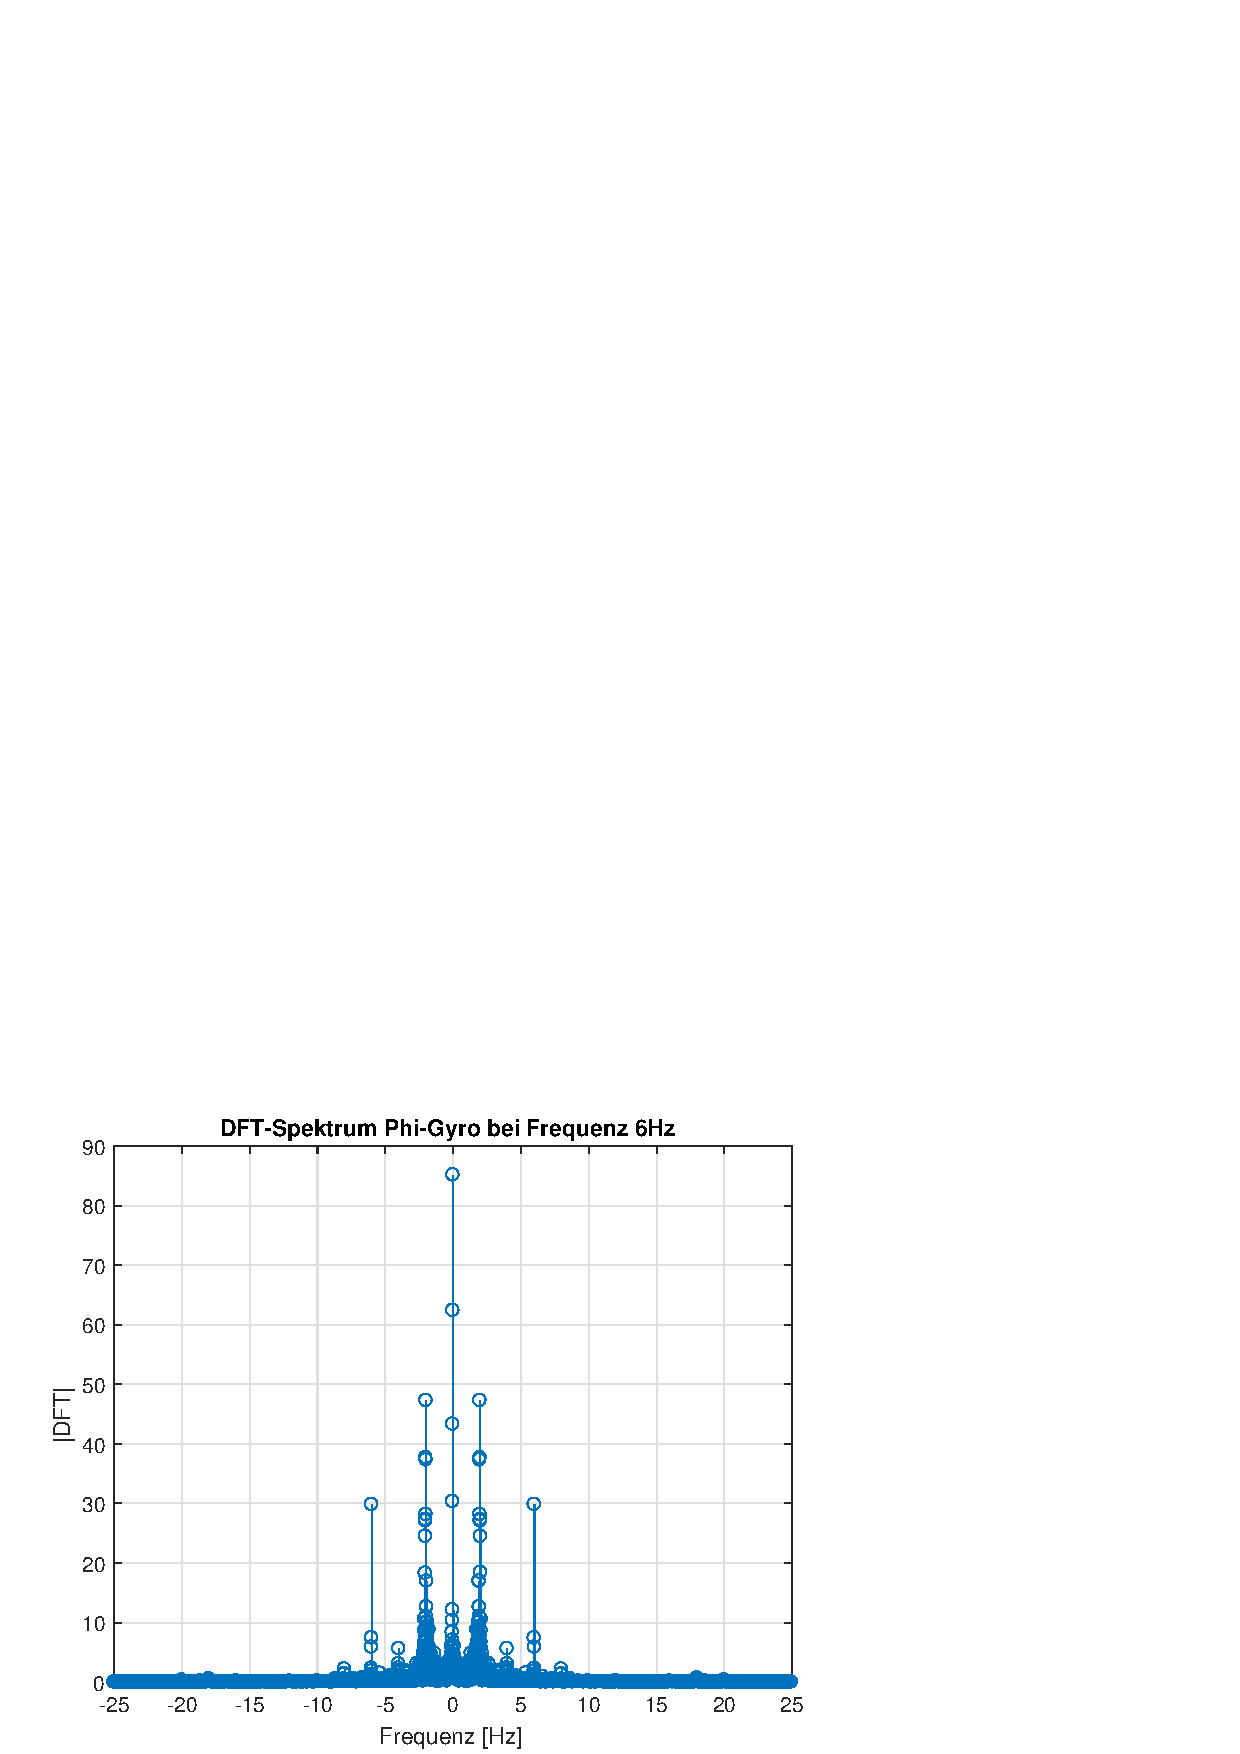
\includegraphics[width=0.5\linewidth]{img/dft_phi_g_7}
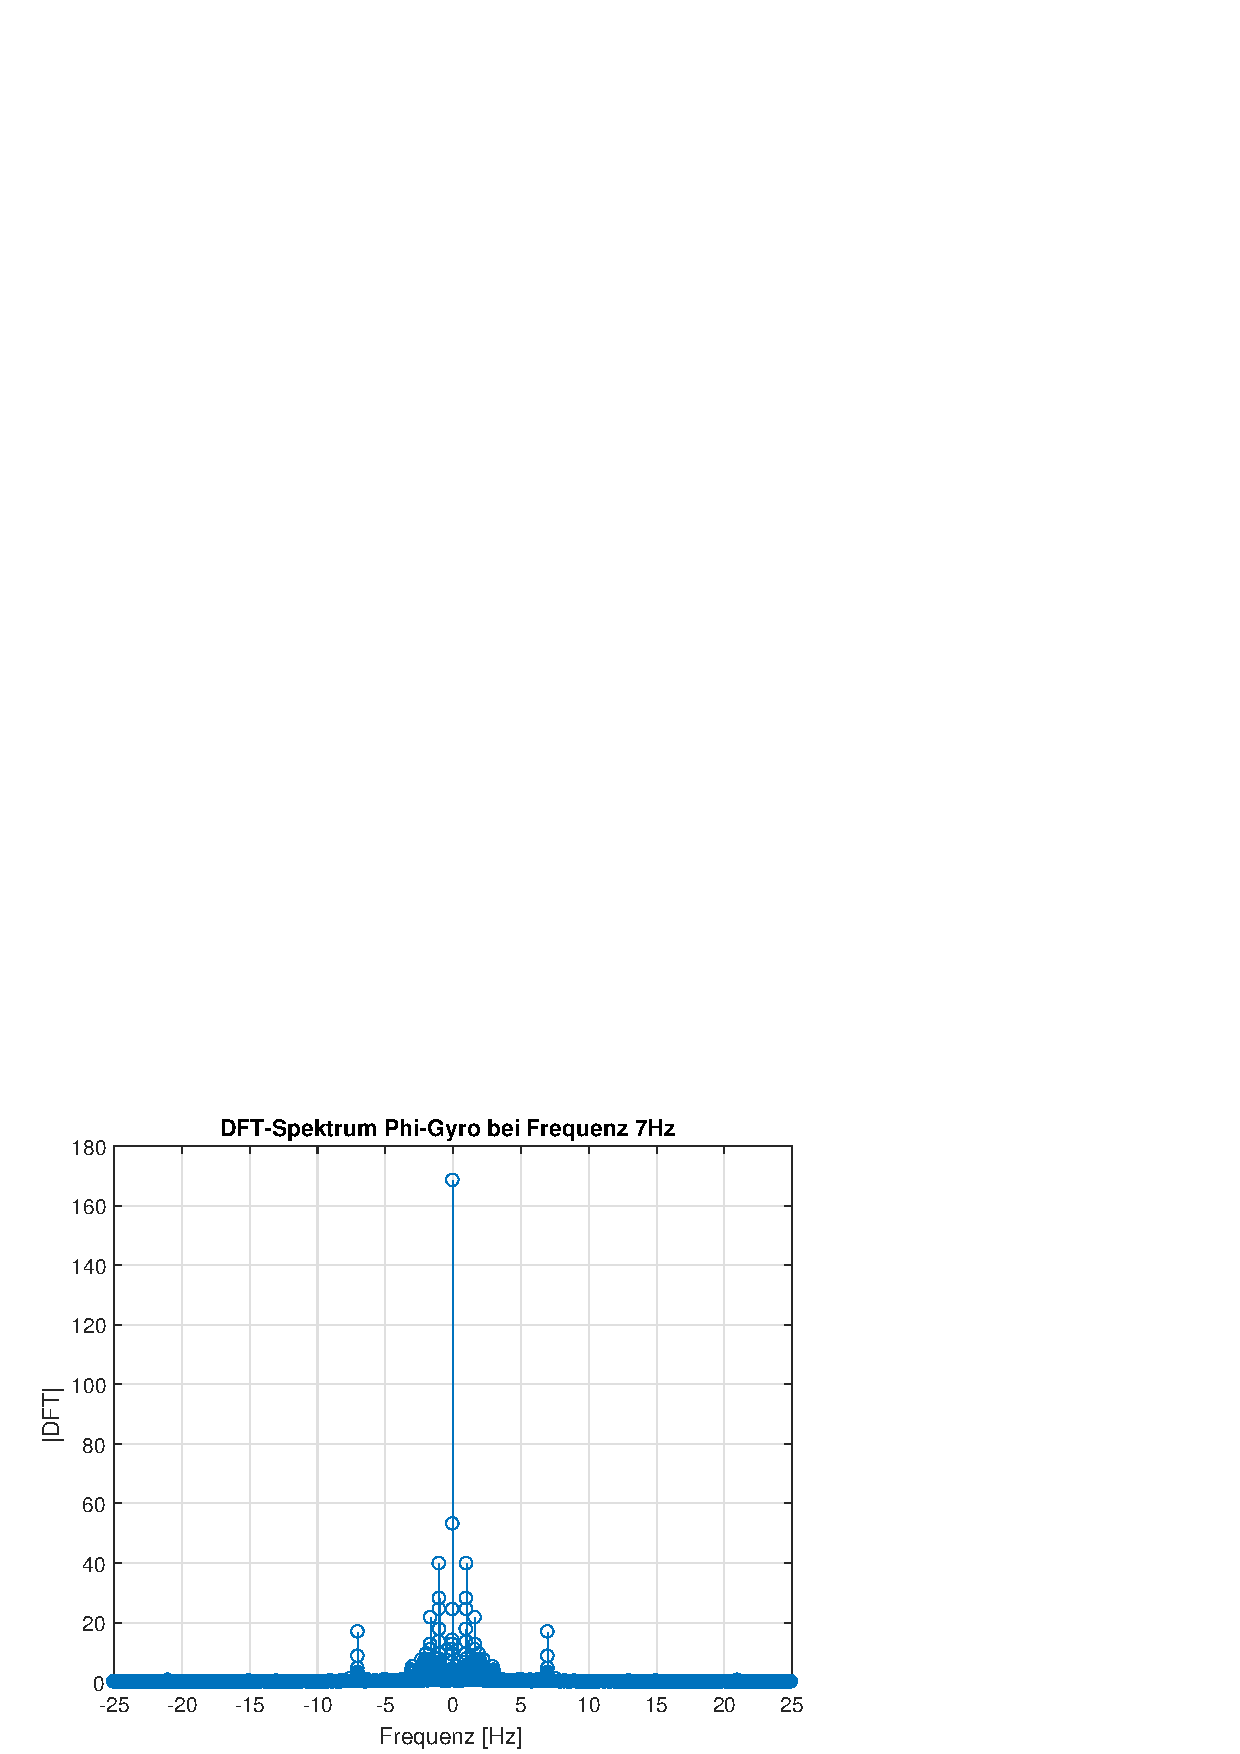
\includegraphics[width=0.5\linewidth]{img/dft_phi_g_8}
\end{figure}
\begin{figure}[h!]
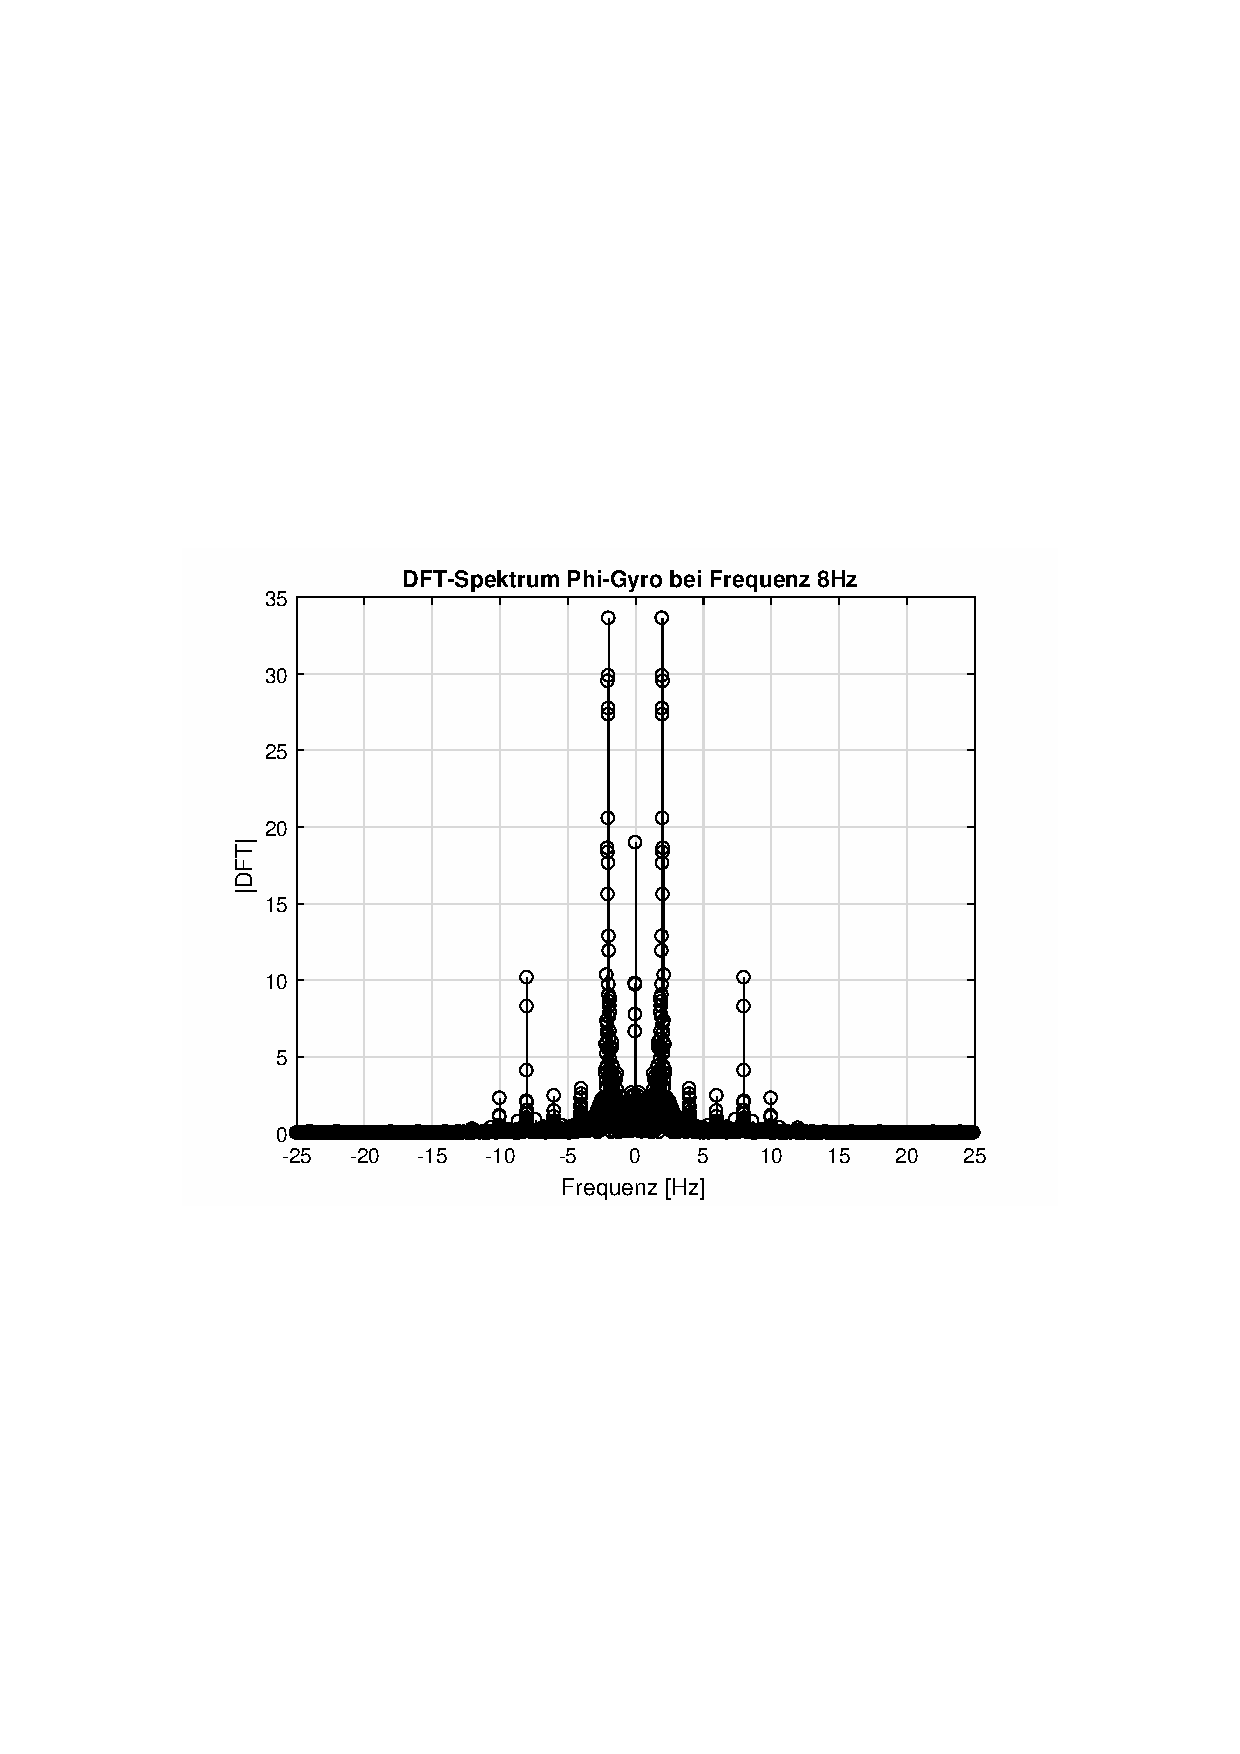
\includegraphics[width=0.5\linewidth]{img/dft_phi_g_9}
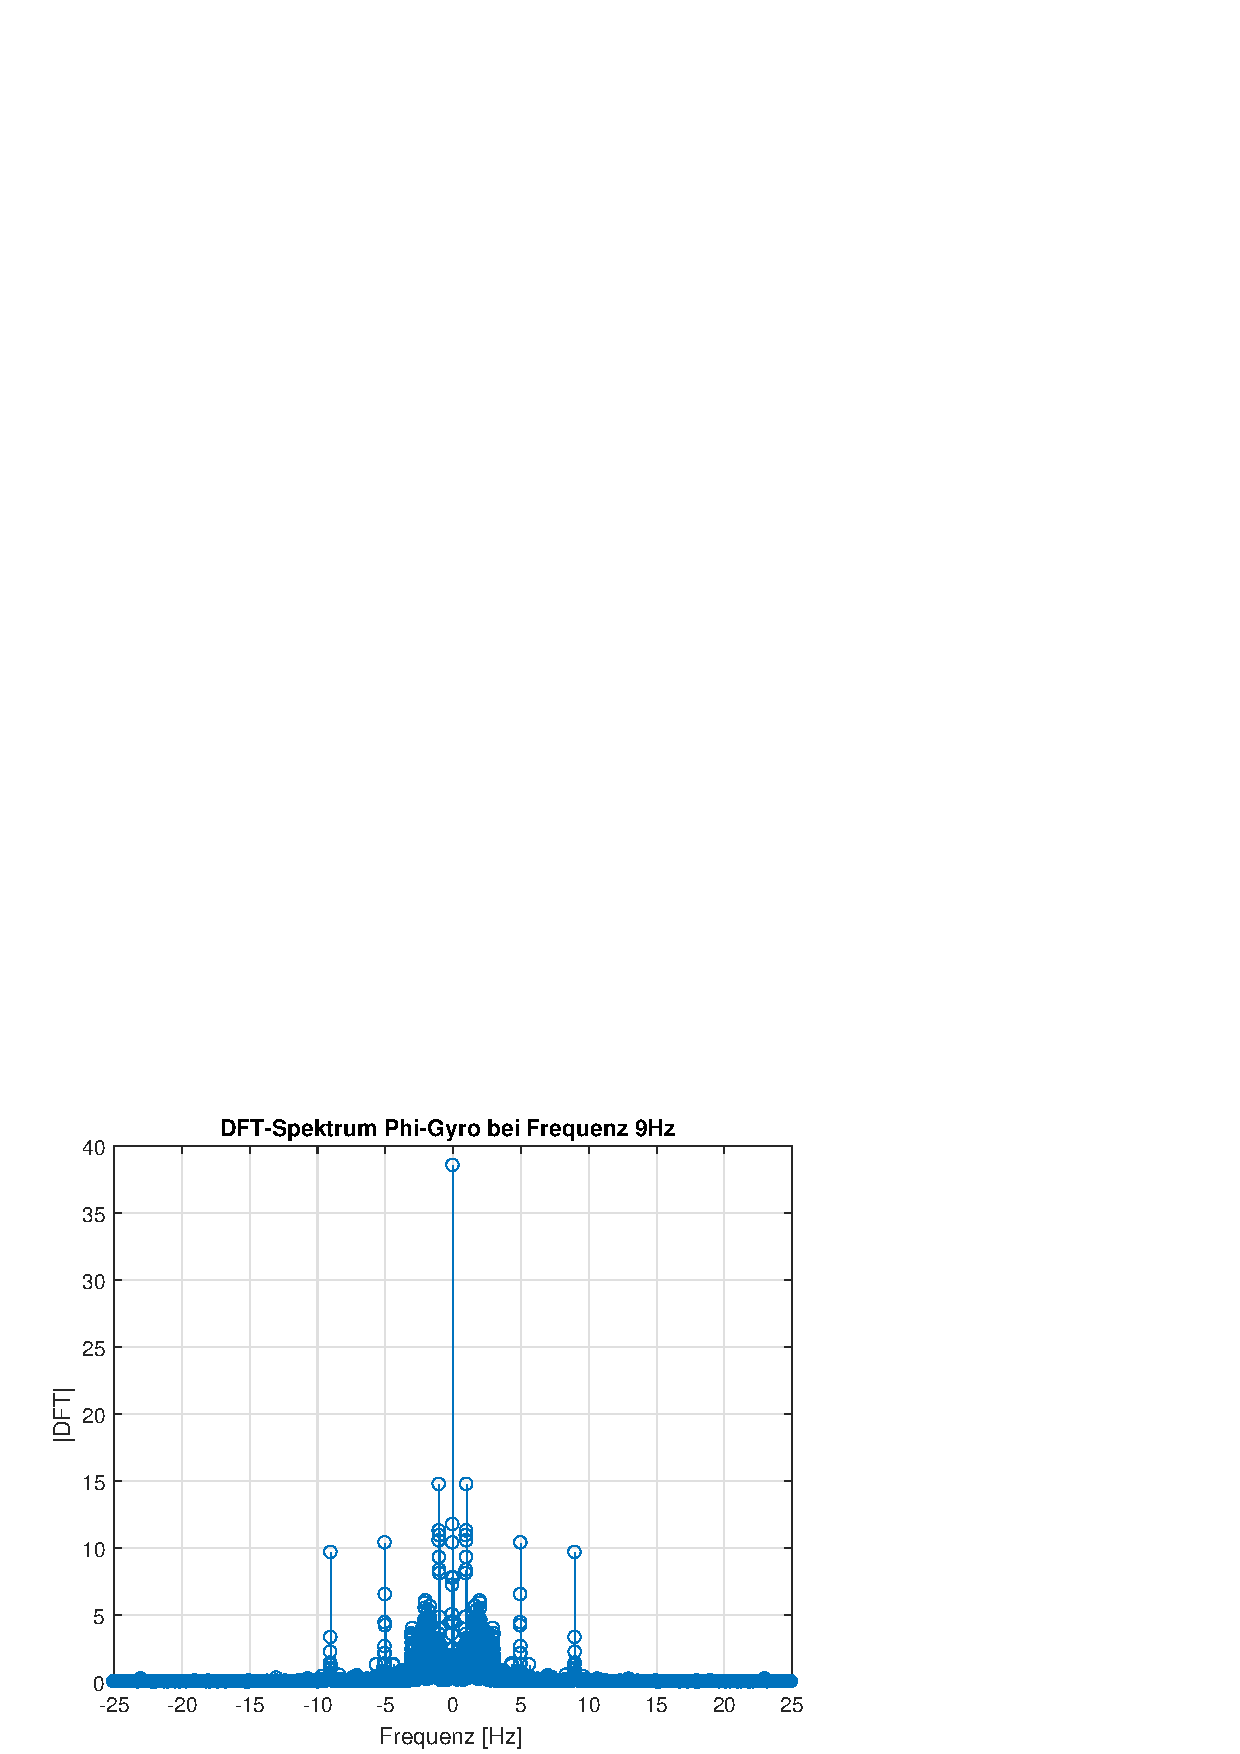
\includegraphics[width=0.5\linewidth]{img/dft_phi_g_10}
\end{figure}
\begin{figure}[h!]
\centering
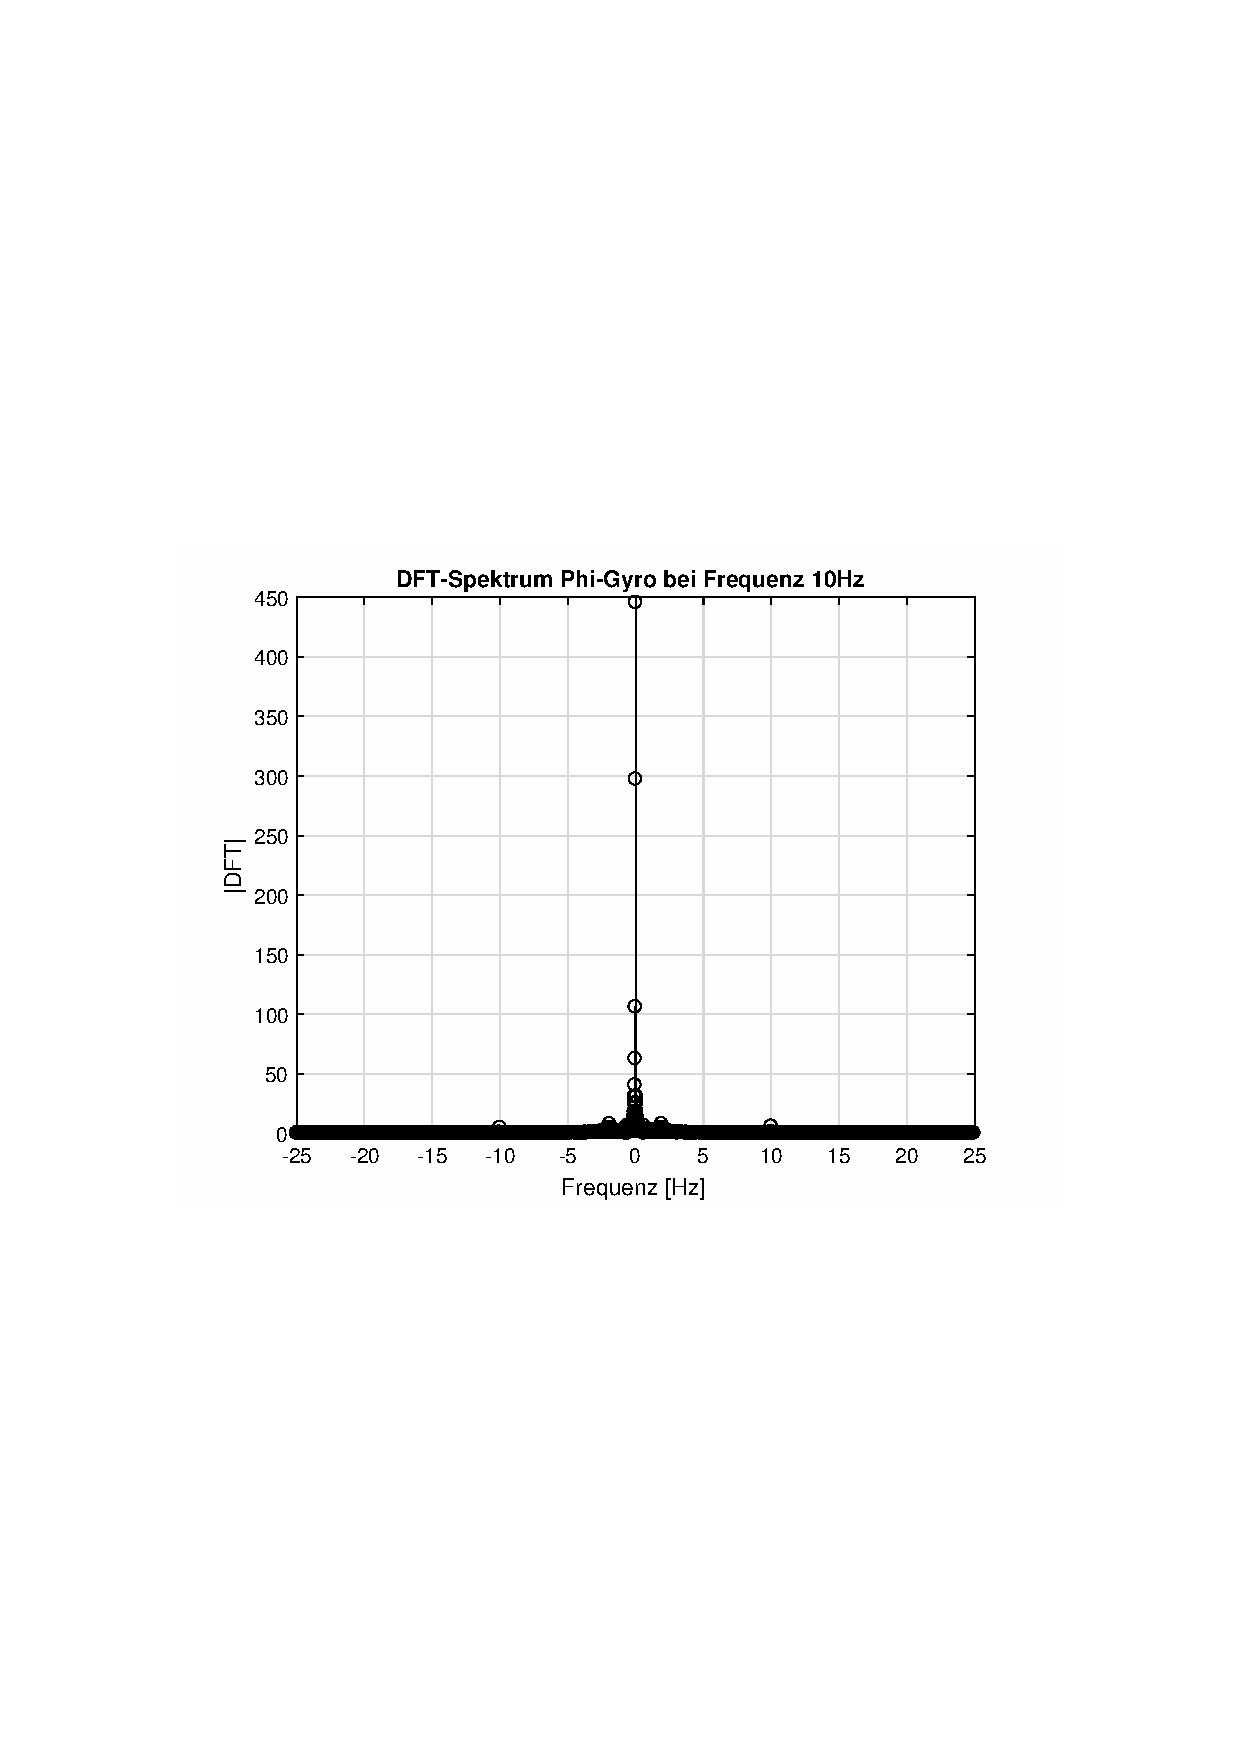
\includegraphics[width=0.5\linewidth]{img/dft_phi_g_11}
\end{figure}

\newpage
\subsection{Leistungsdichtespektren von $\varphi$ bei $T_M = sin(2\pi\cdot f\cdot t)$}
\begin{figure}[h!]
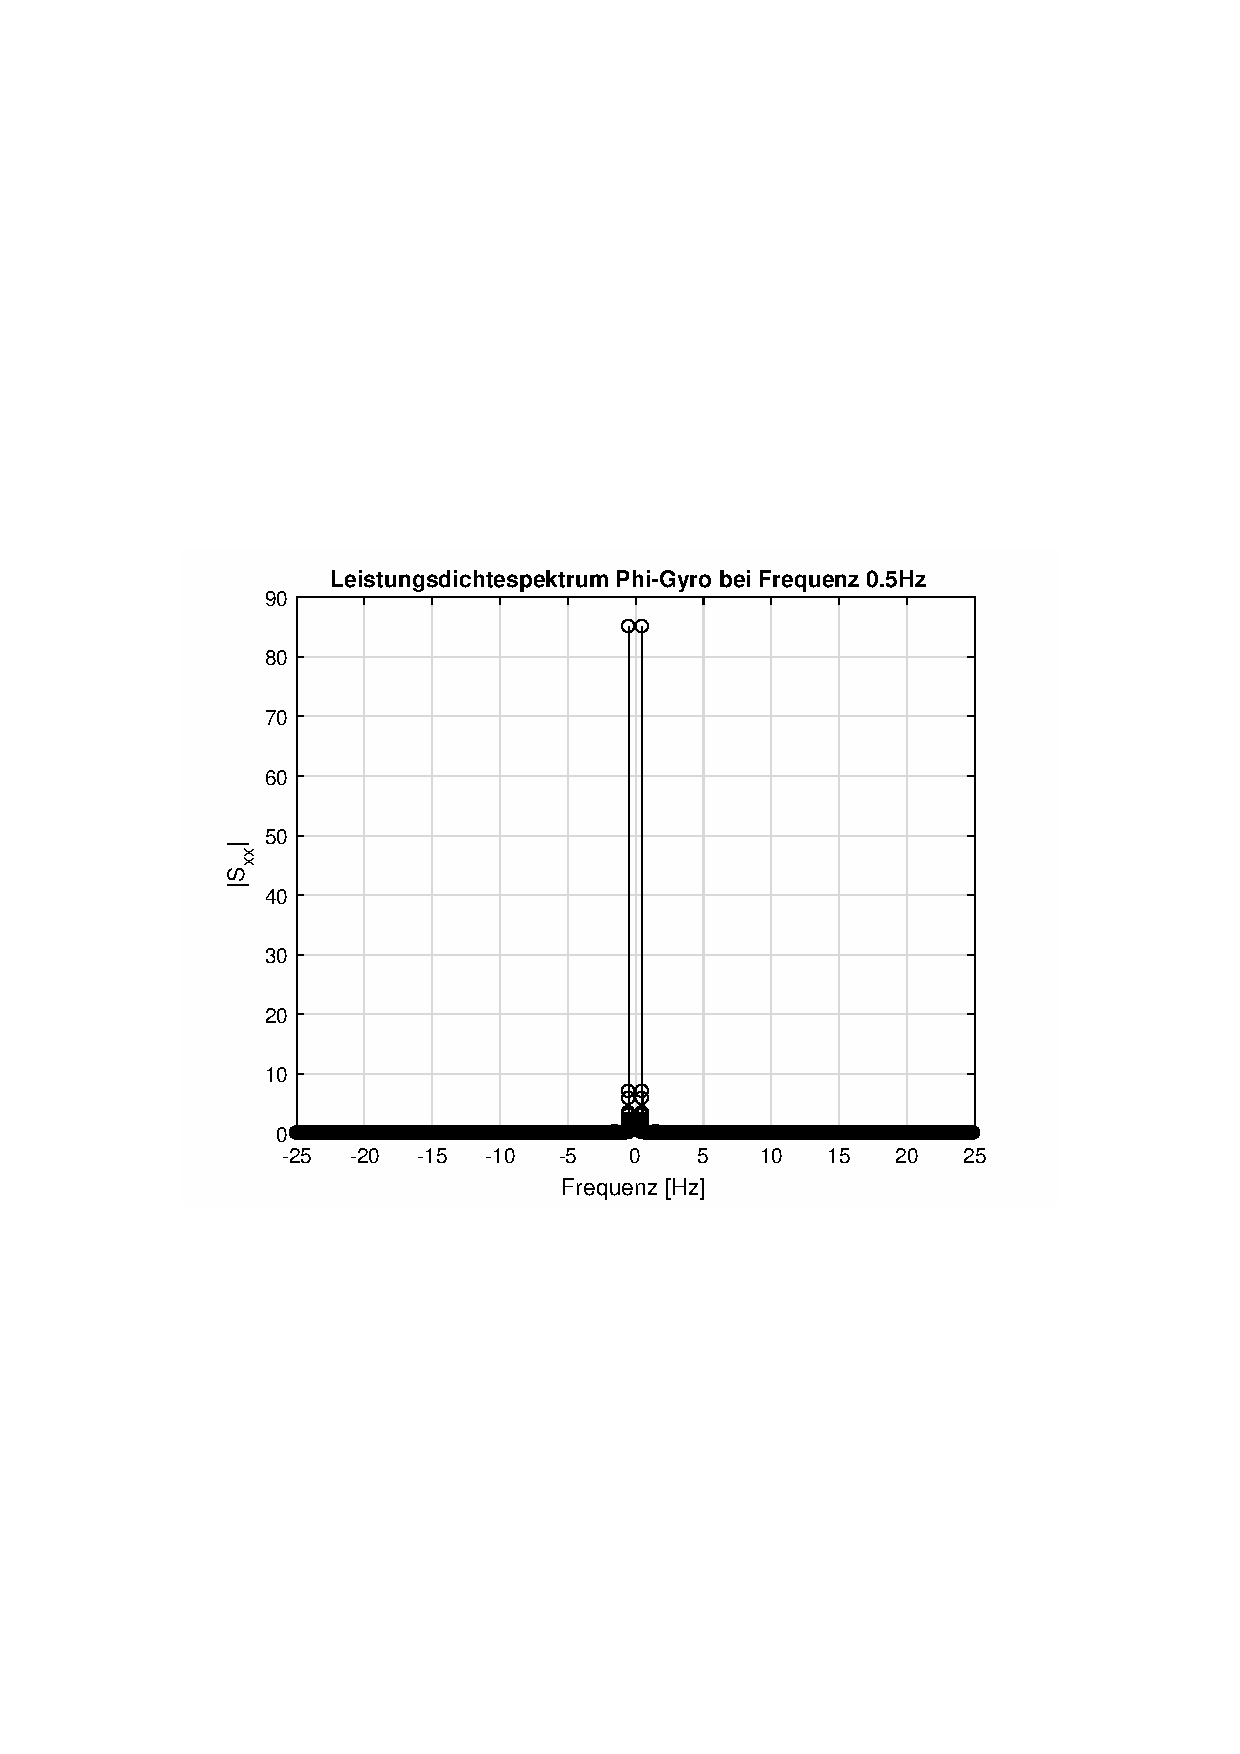
\includegraphics[width=0.5\linewidth]{img/lds_phi_g_1}
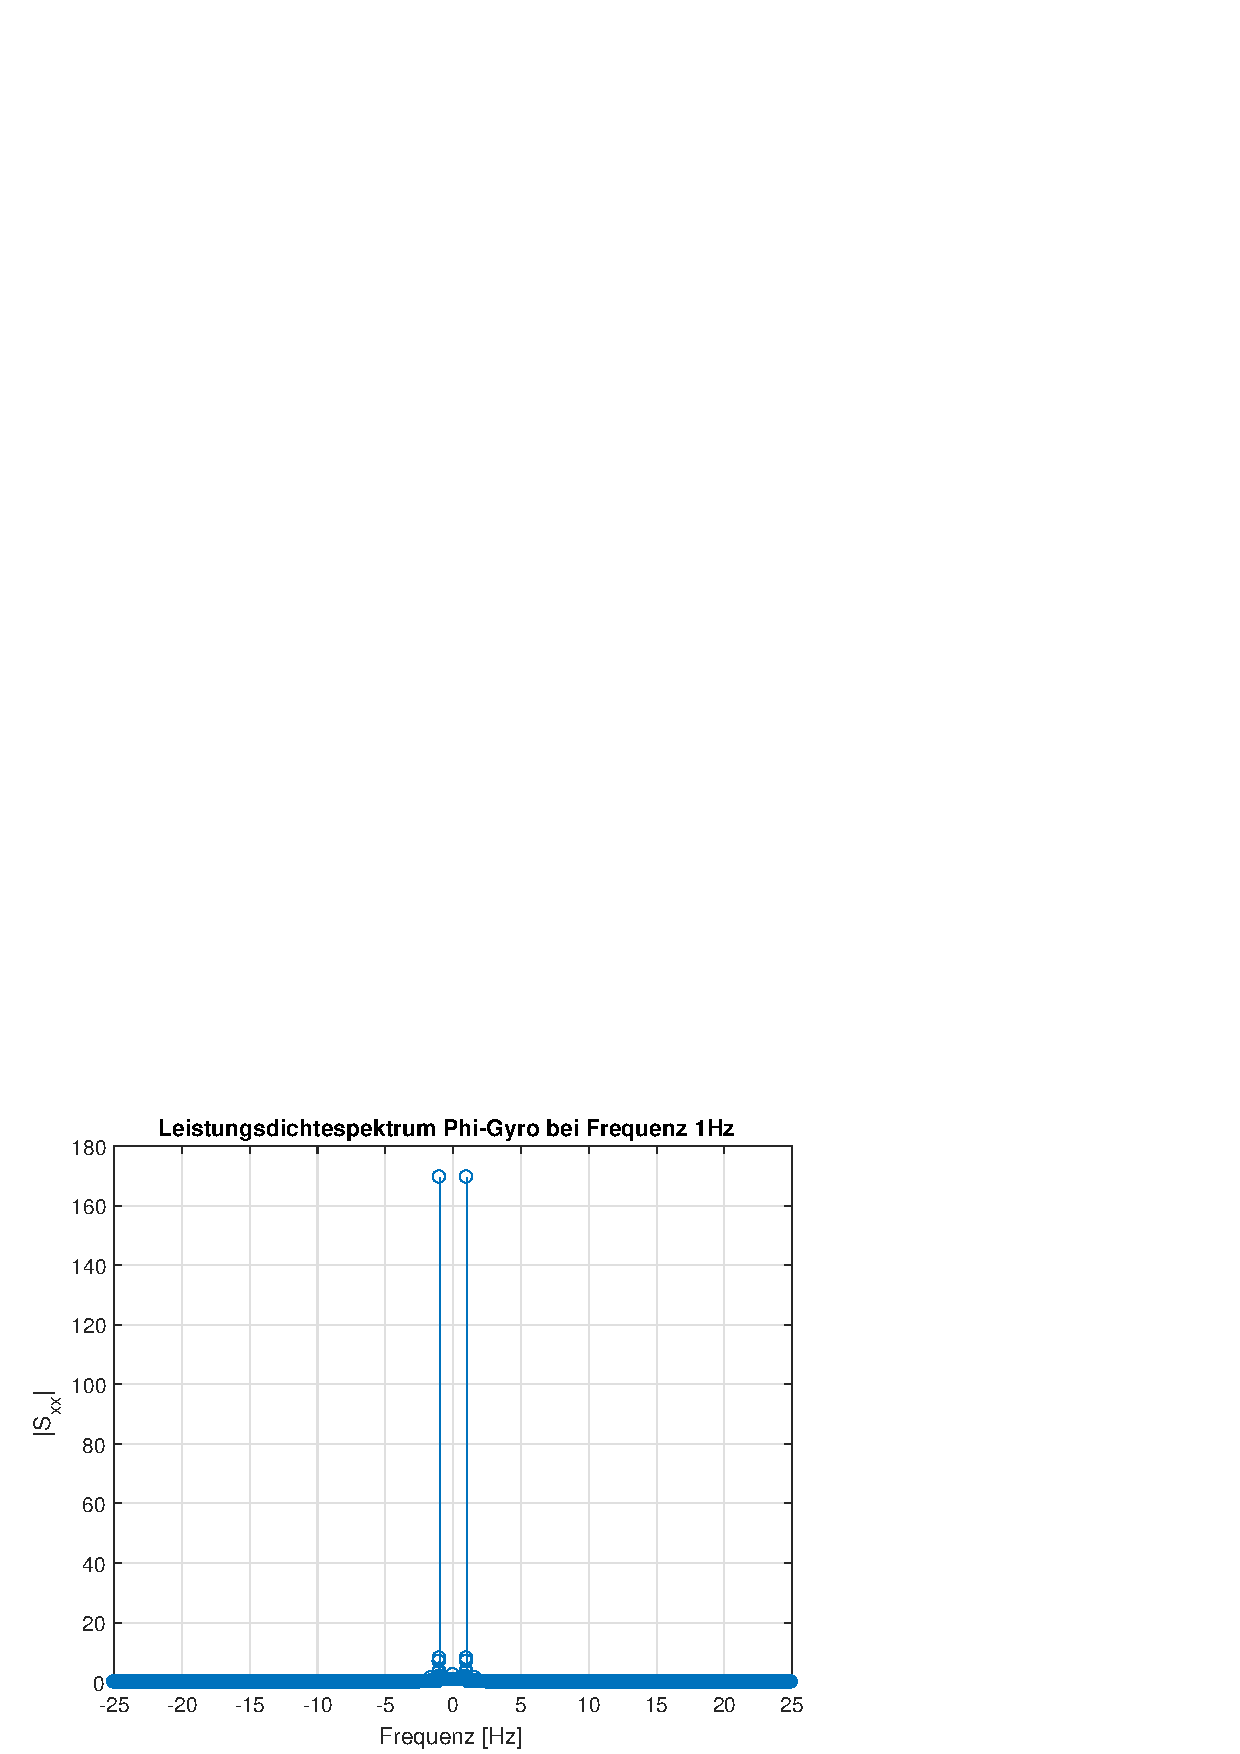
\includegraphics[width=0.5\linewidth]{img/lds_phi_g_2}
\end{figure}
\begin{figure}[h!]
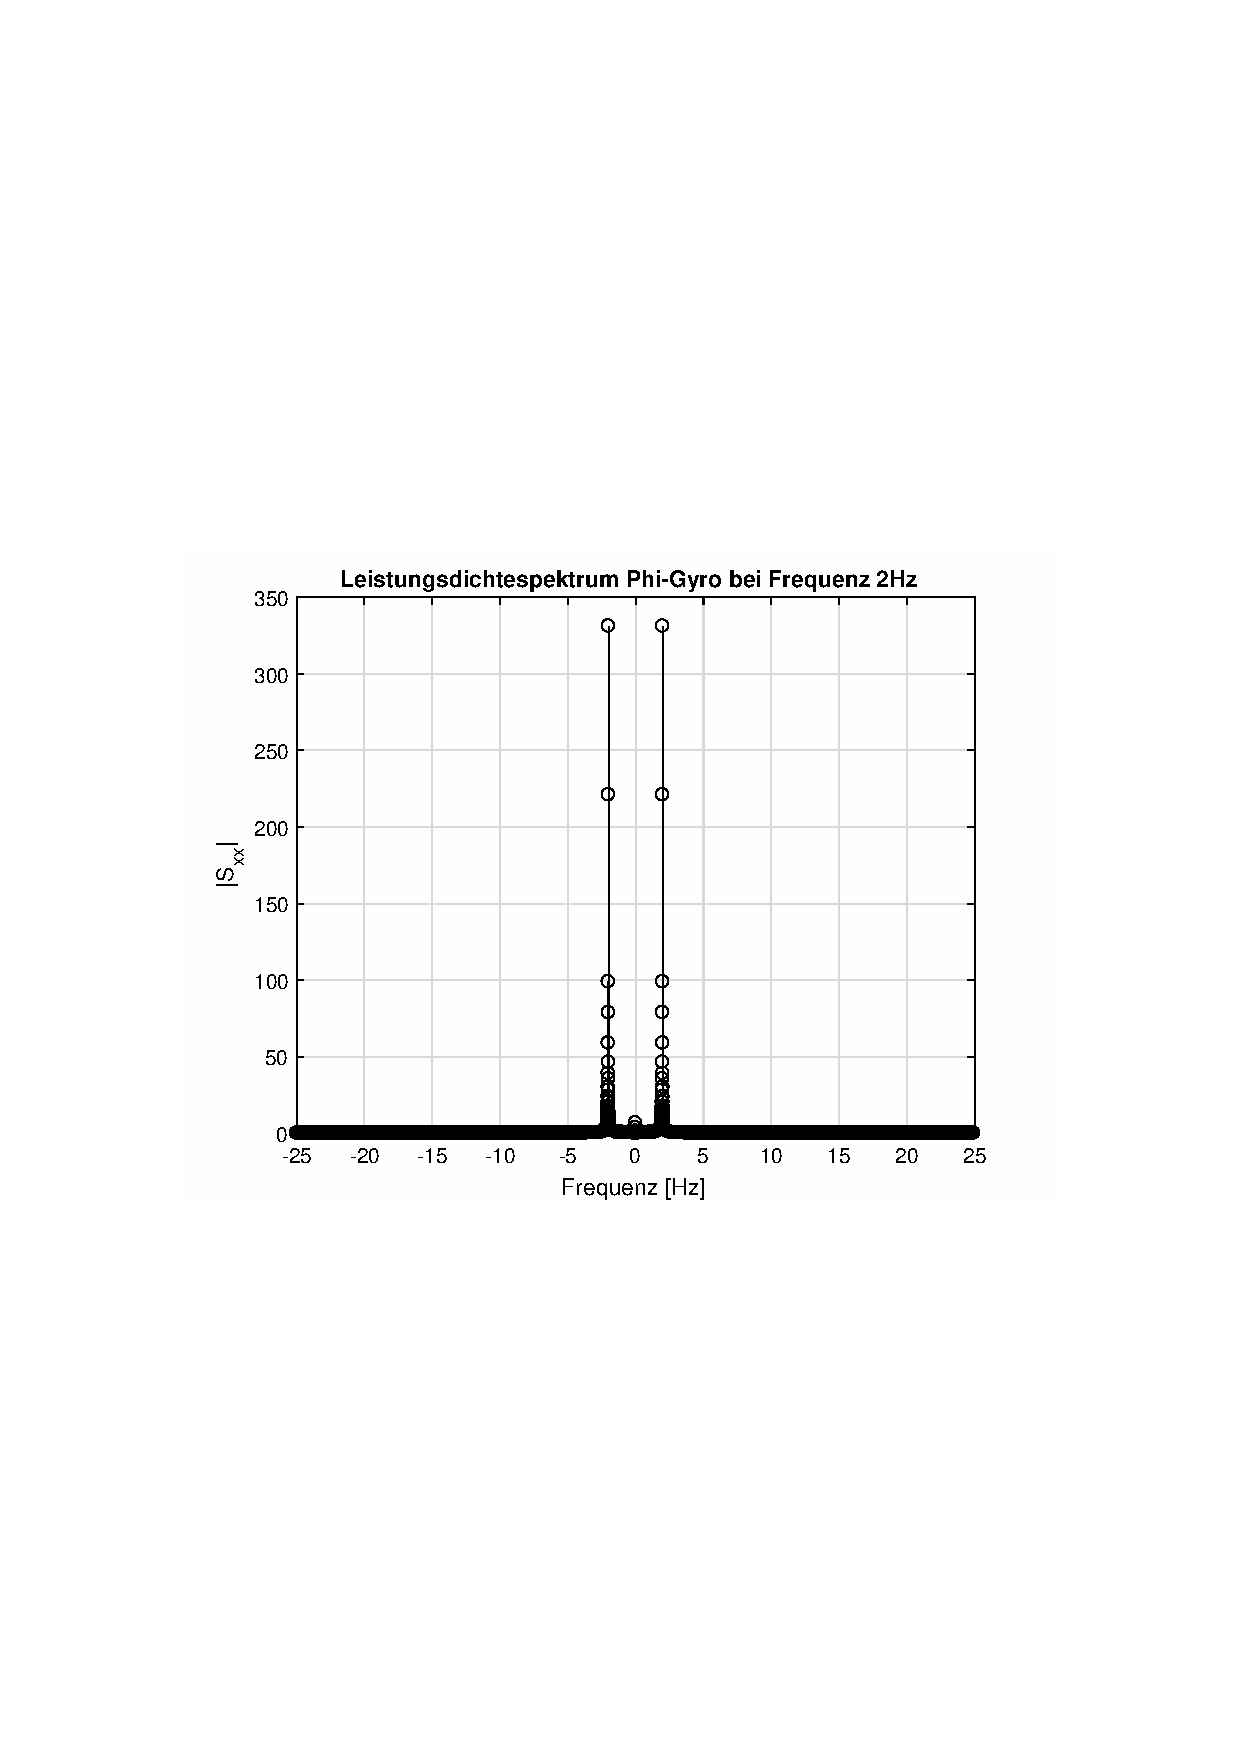
\includegraphics[width=0.5\linewidth]{img/lds_phi_g_3}
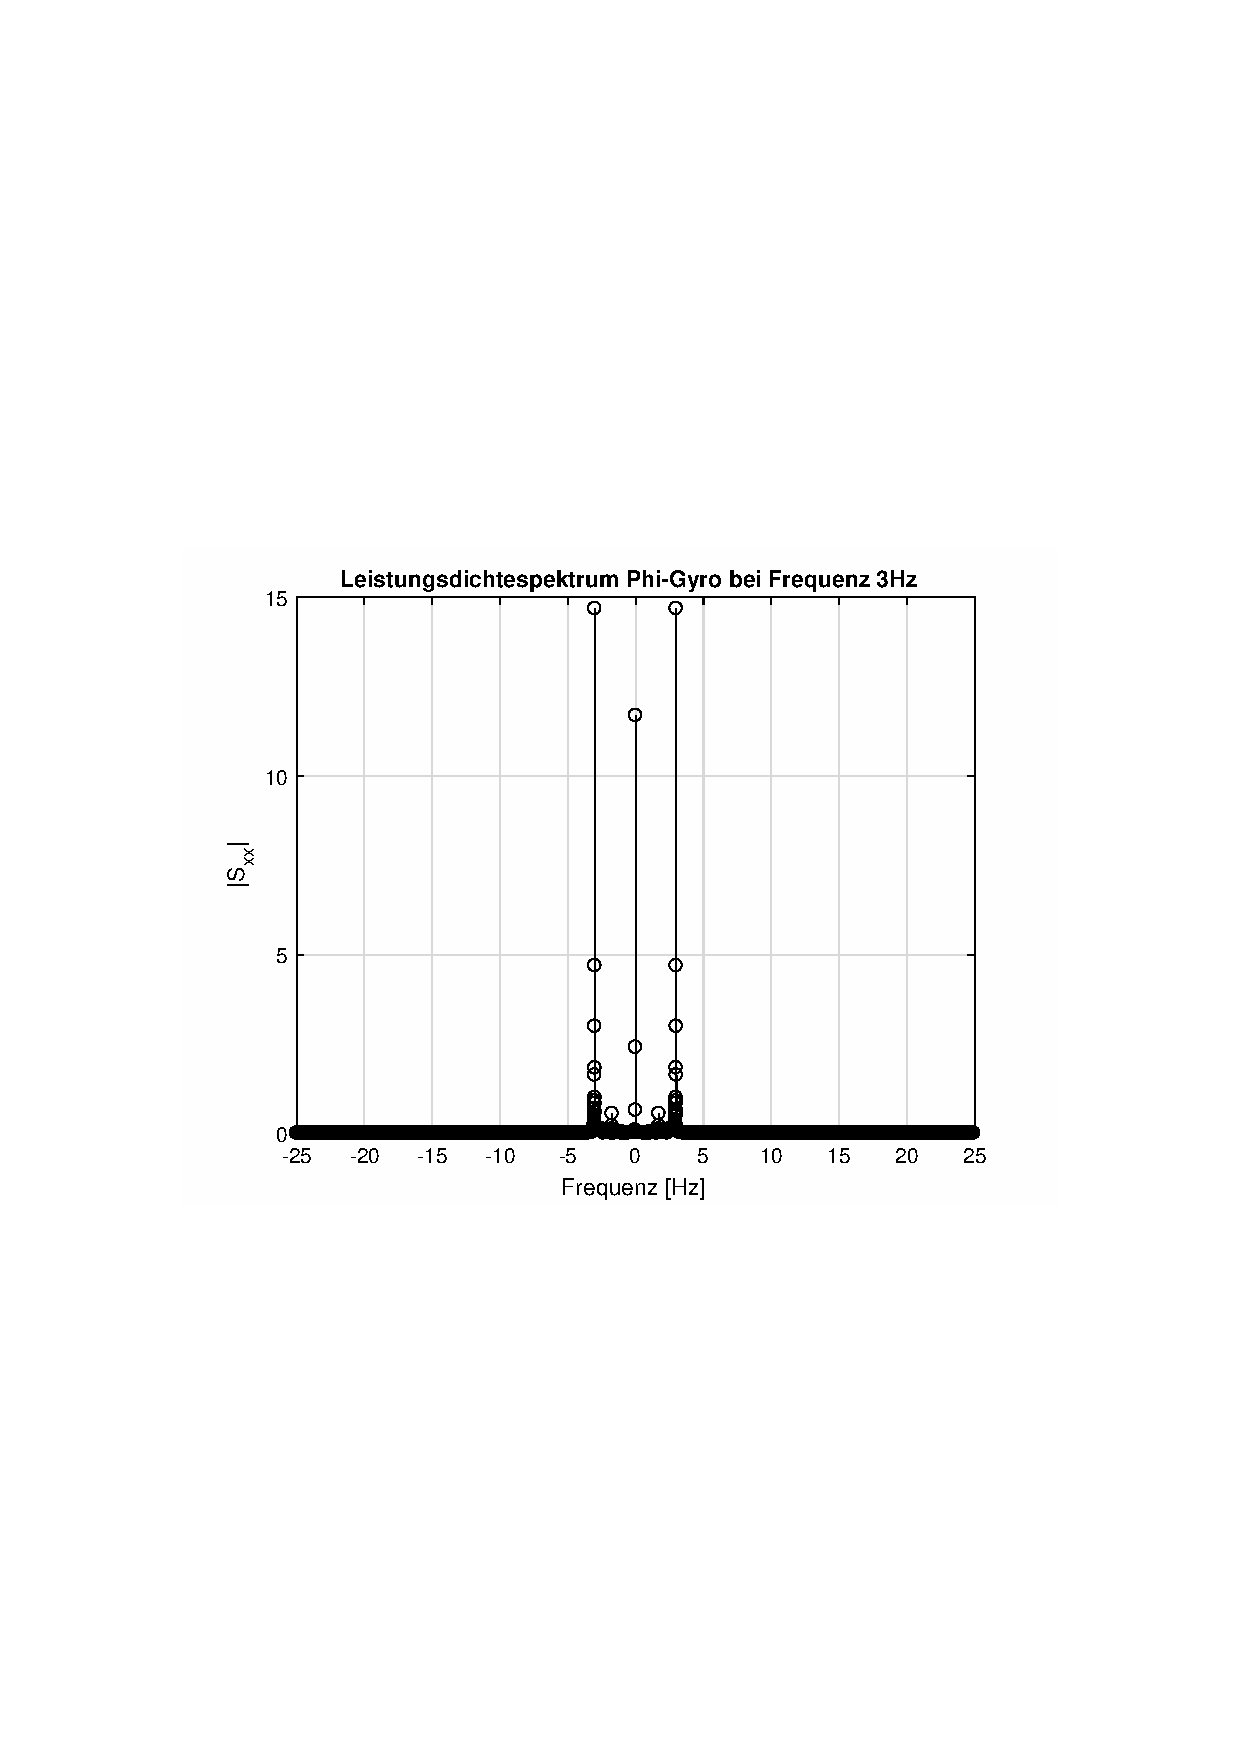
\includegraphics[width=0.5\linewidth]{img/lds_phi_g_4}
\end{figure}
\begin{figure}[h!]
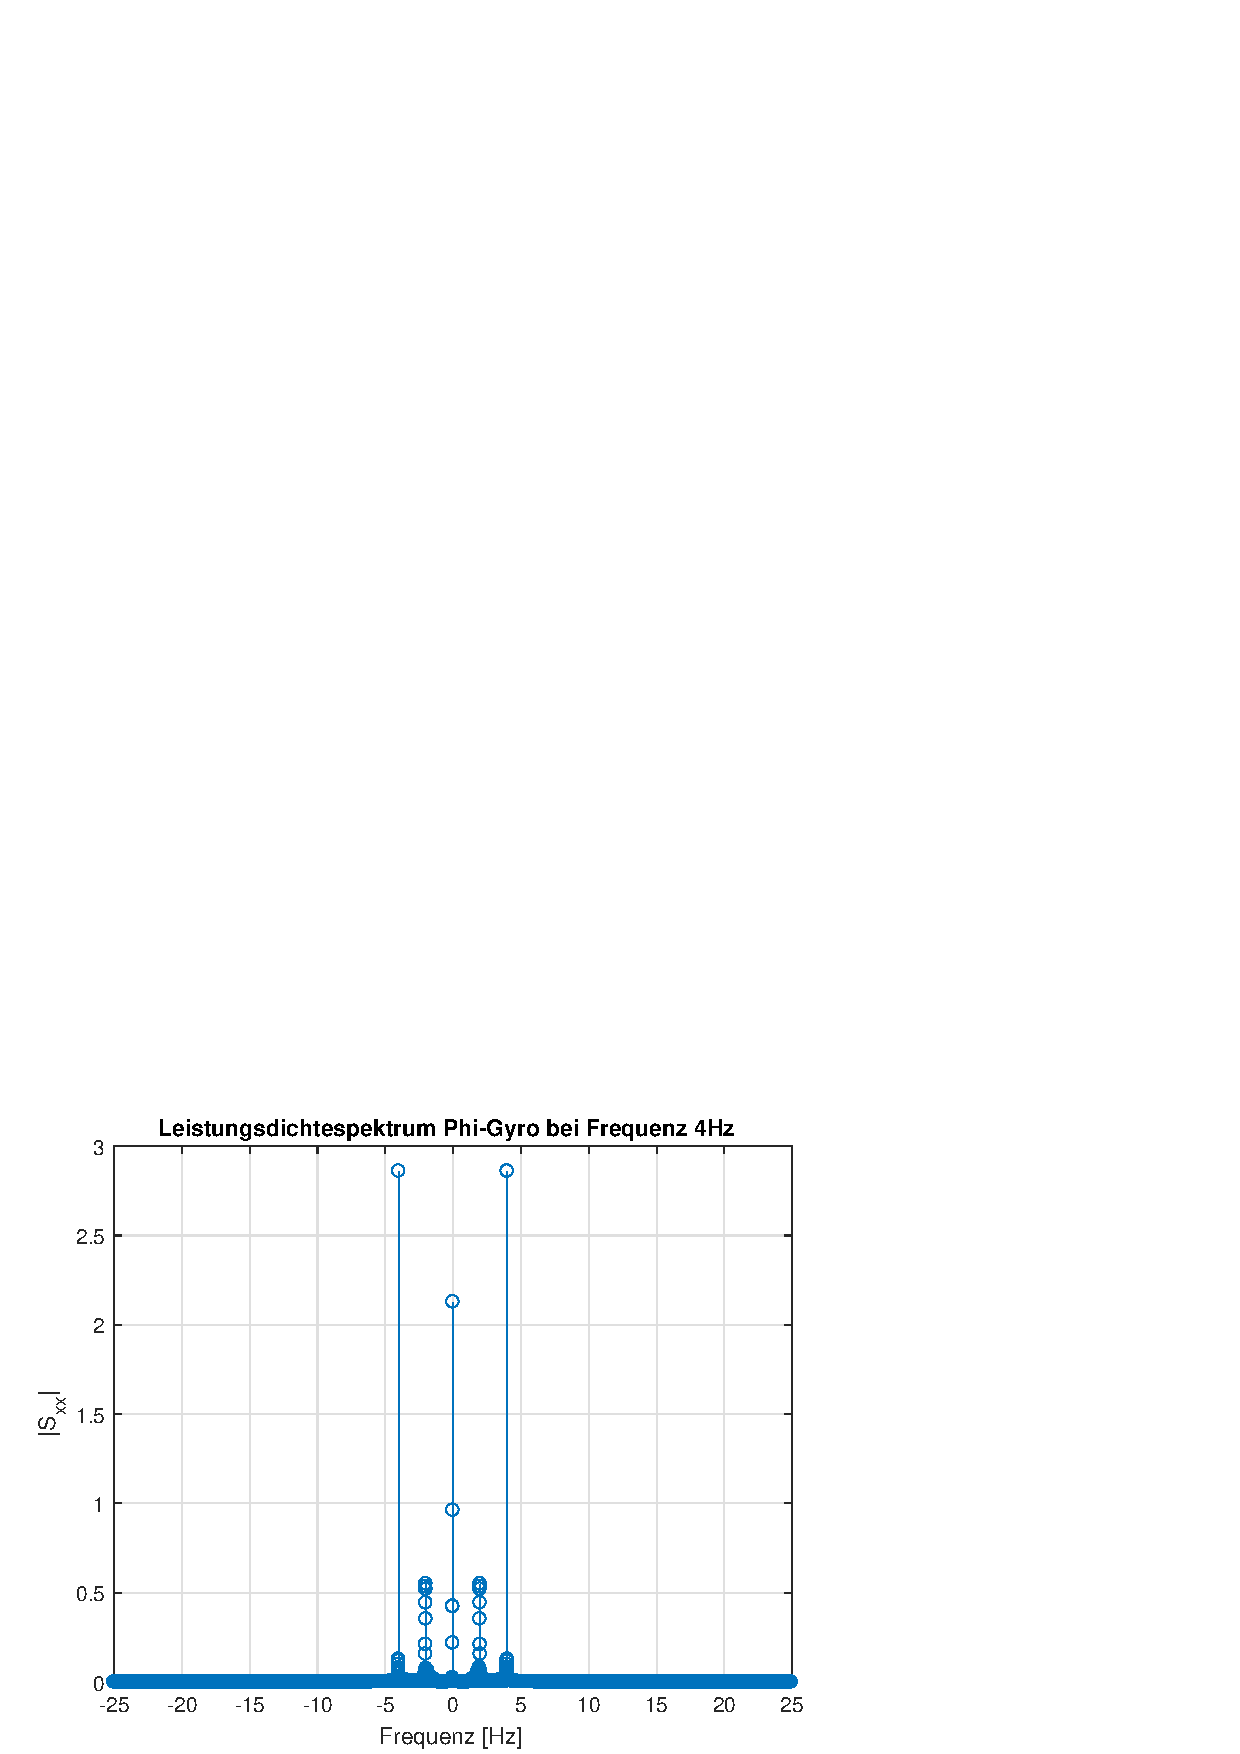
\includegraphics[width=0.5\linewidth]{img/lds_phi_g_5}
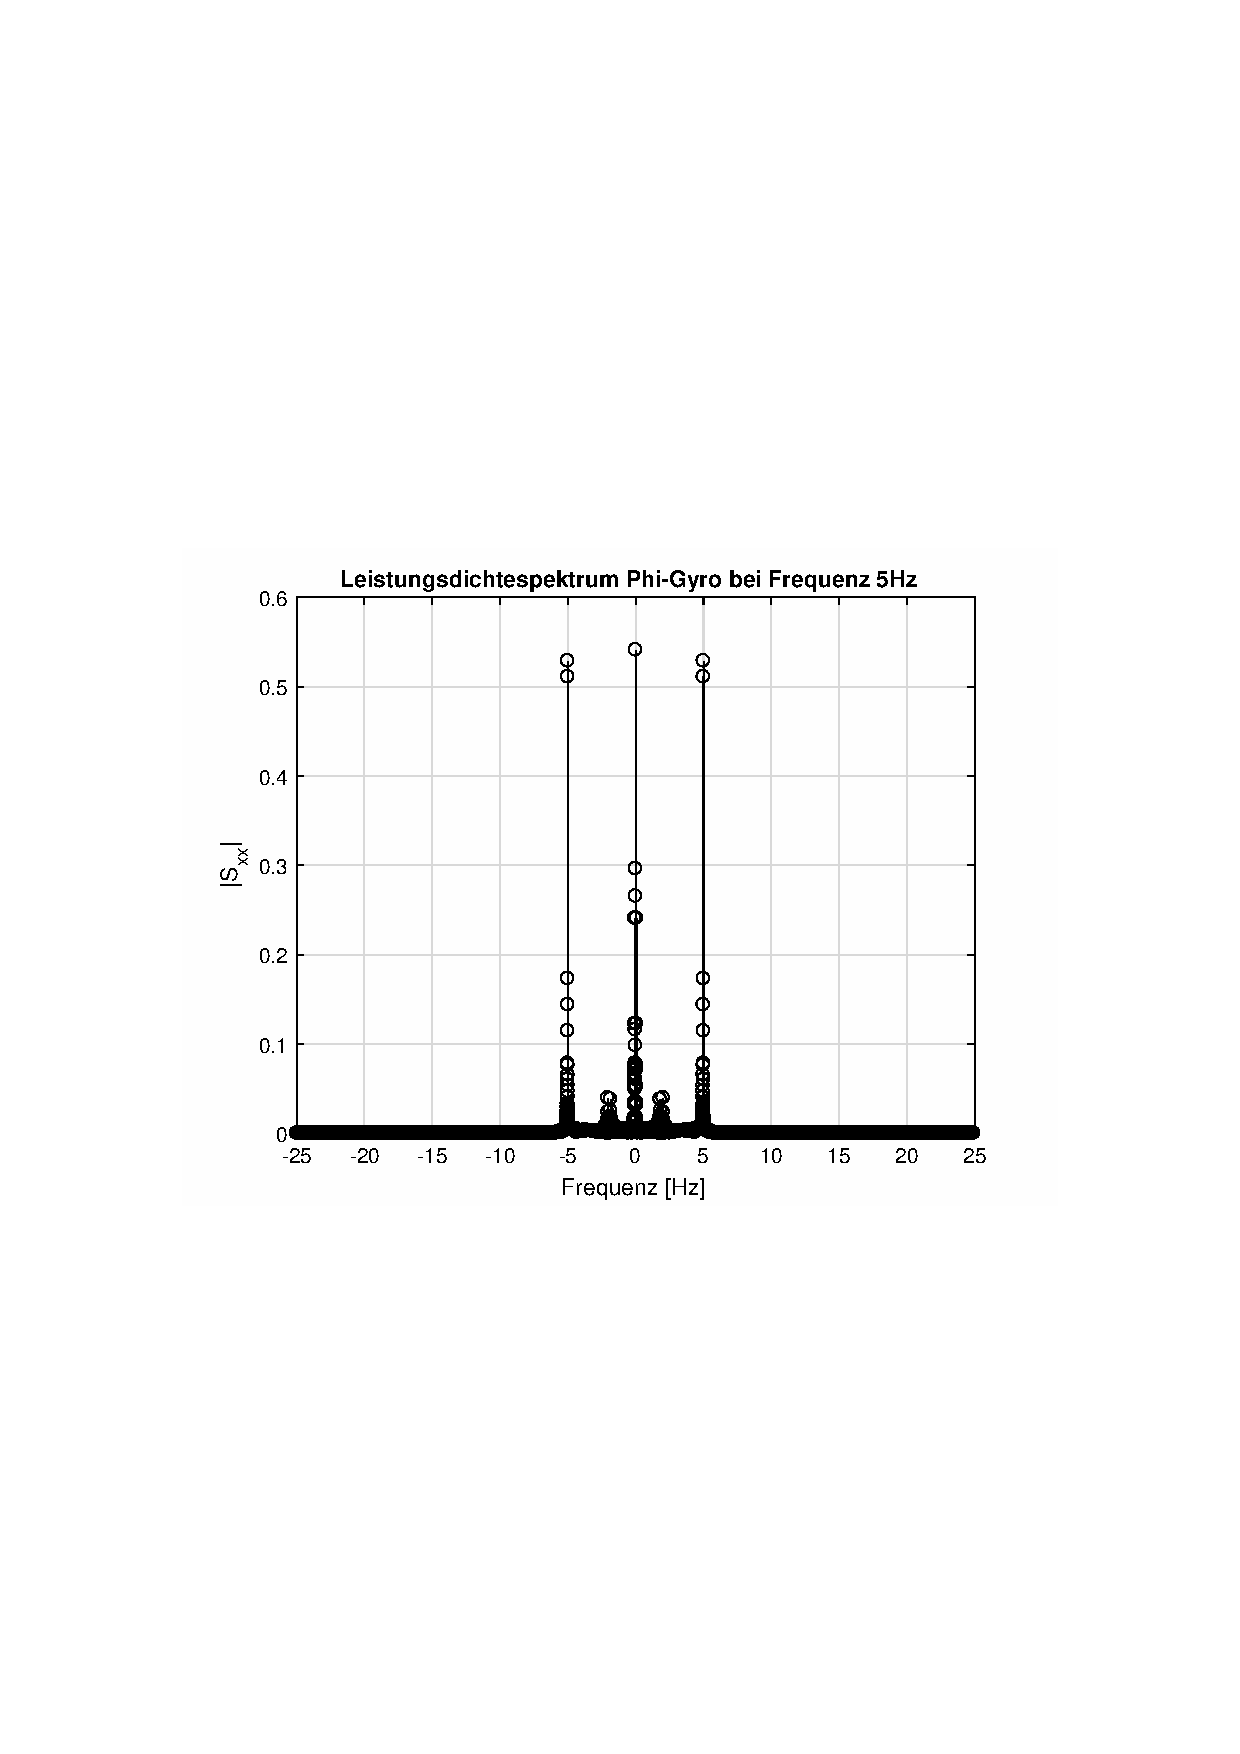
\includegraphics[width=0.5\linewidth]{img/lds_phi_g_6}
\end{figure}
\newpage
\begin{figure}[h!]
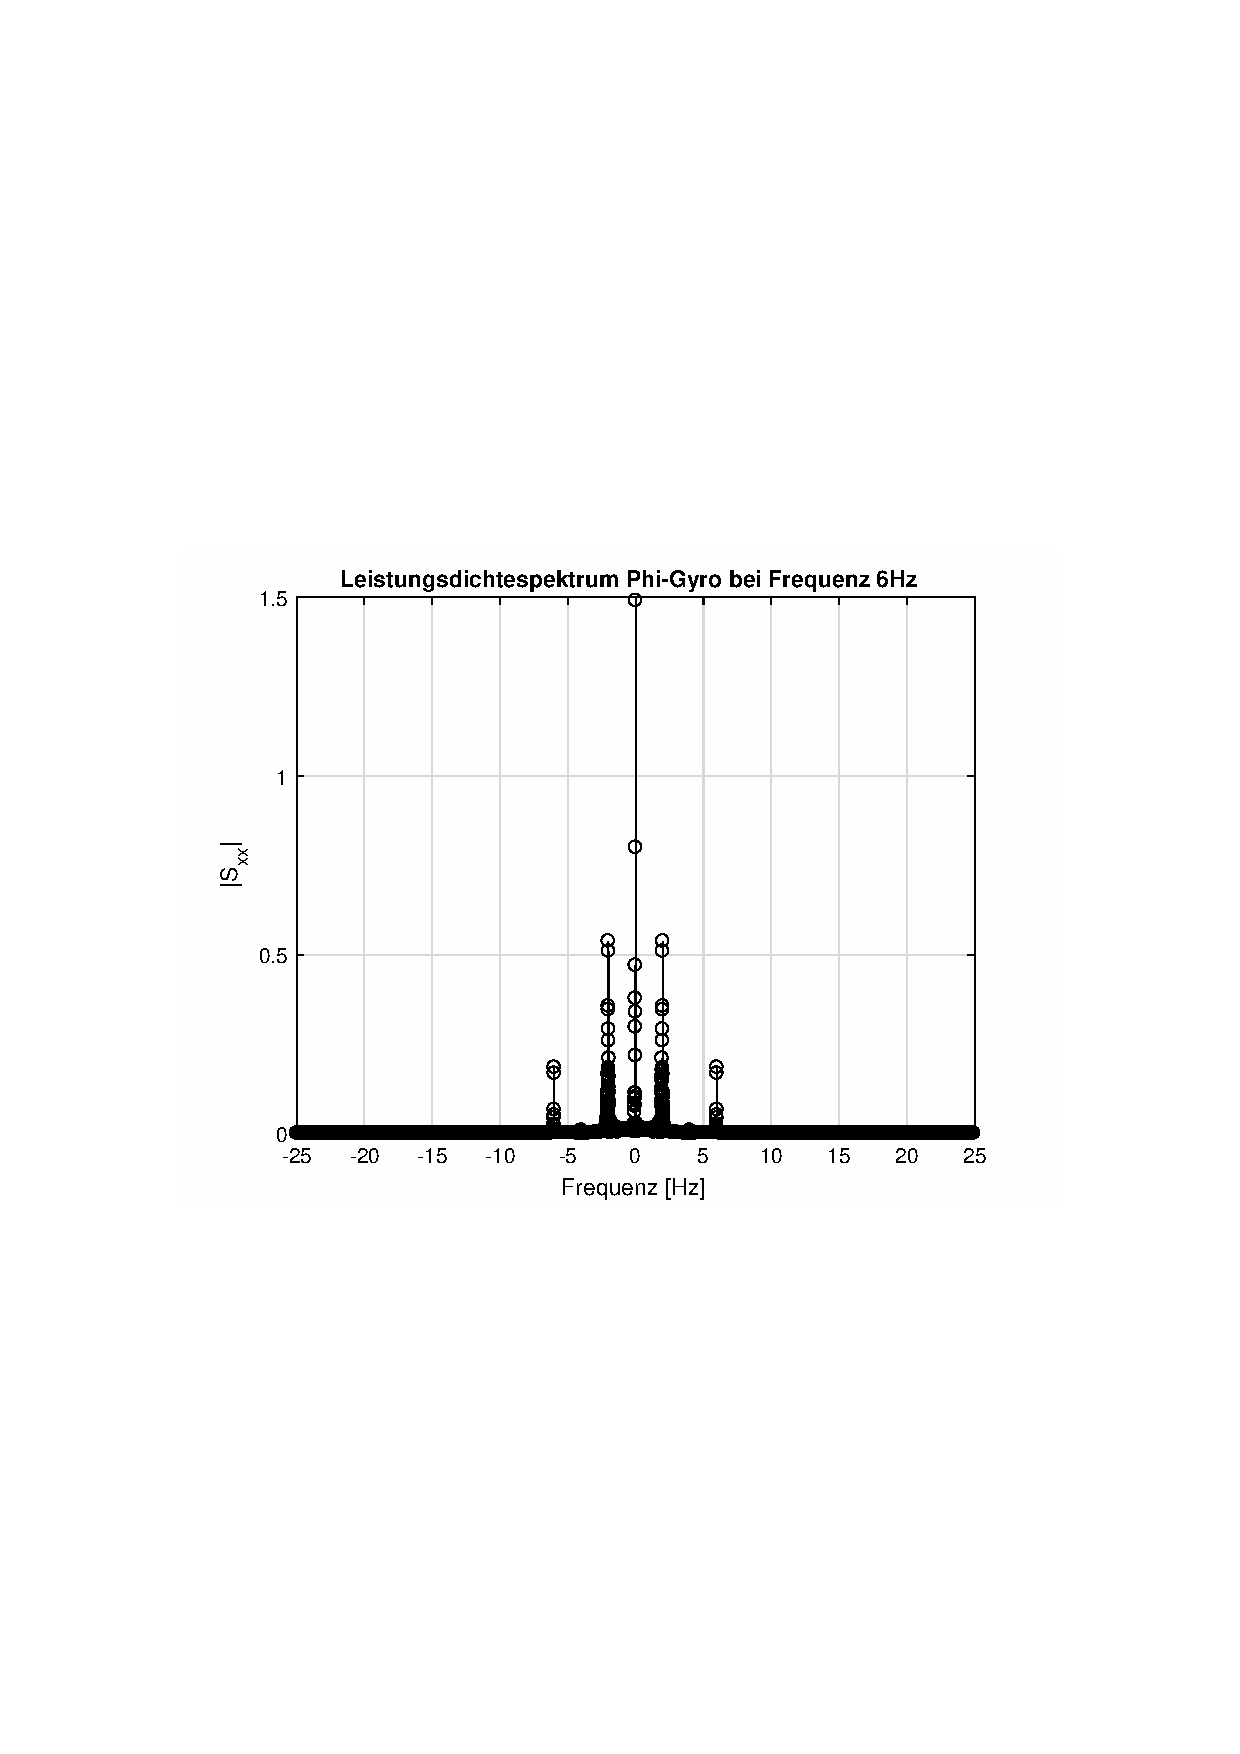
\includegraphics[width=0.5\linewidth]{img/lds_phi_g_7}
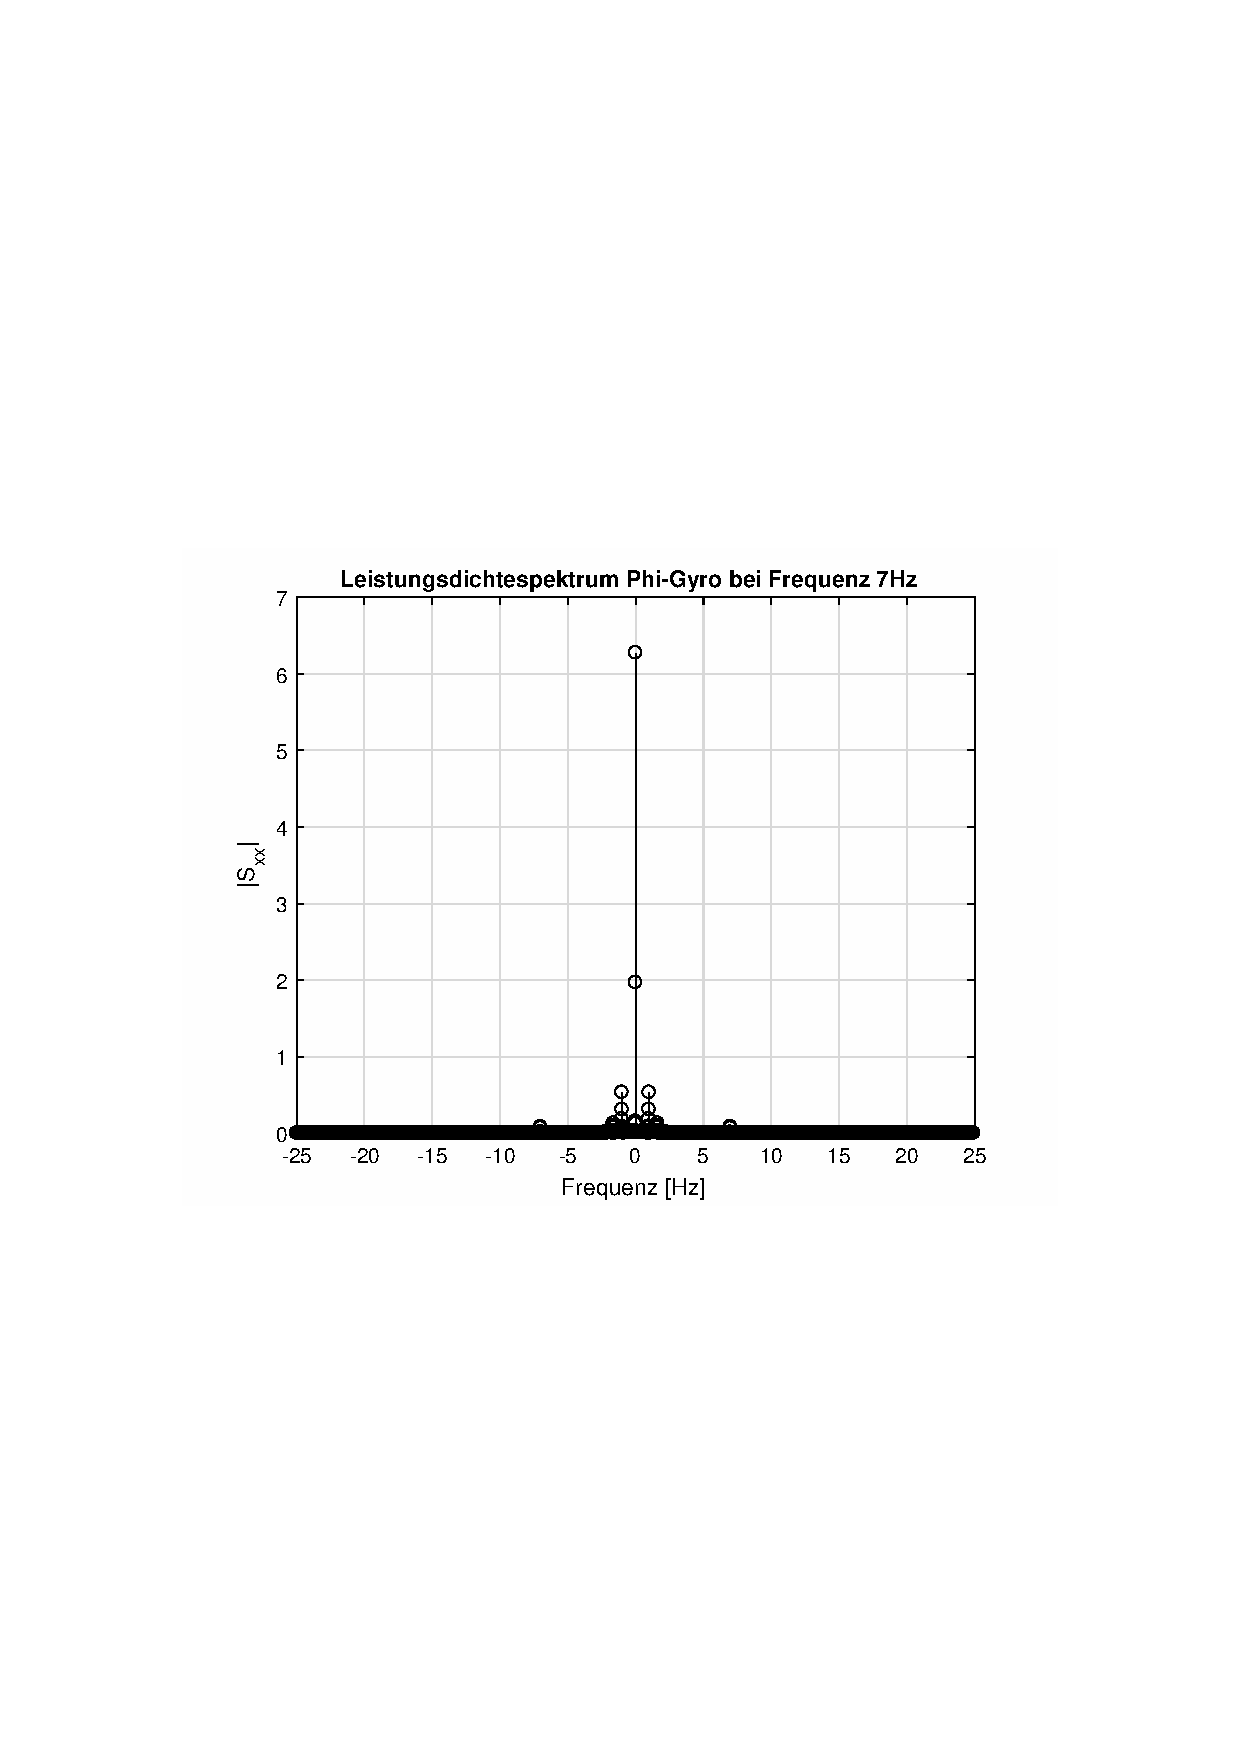
\includegraphics[width=0.5\linewidth]{img/lds_phi_g_8}
\end{figure}
\begin{figure}[h!]
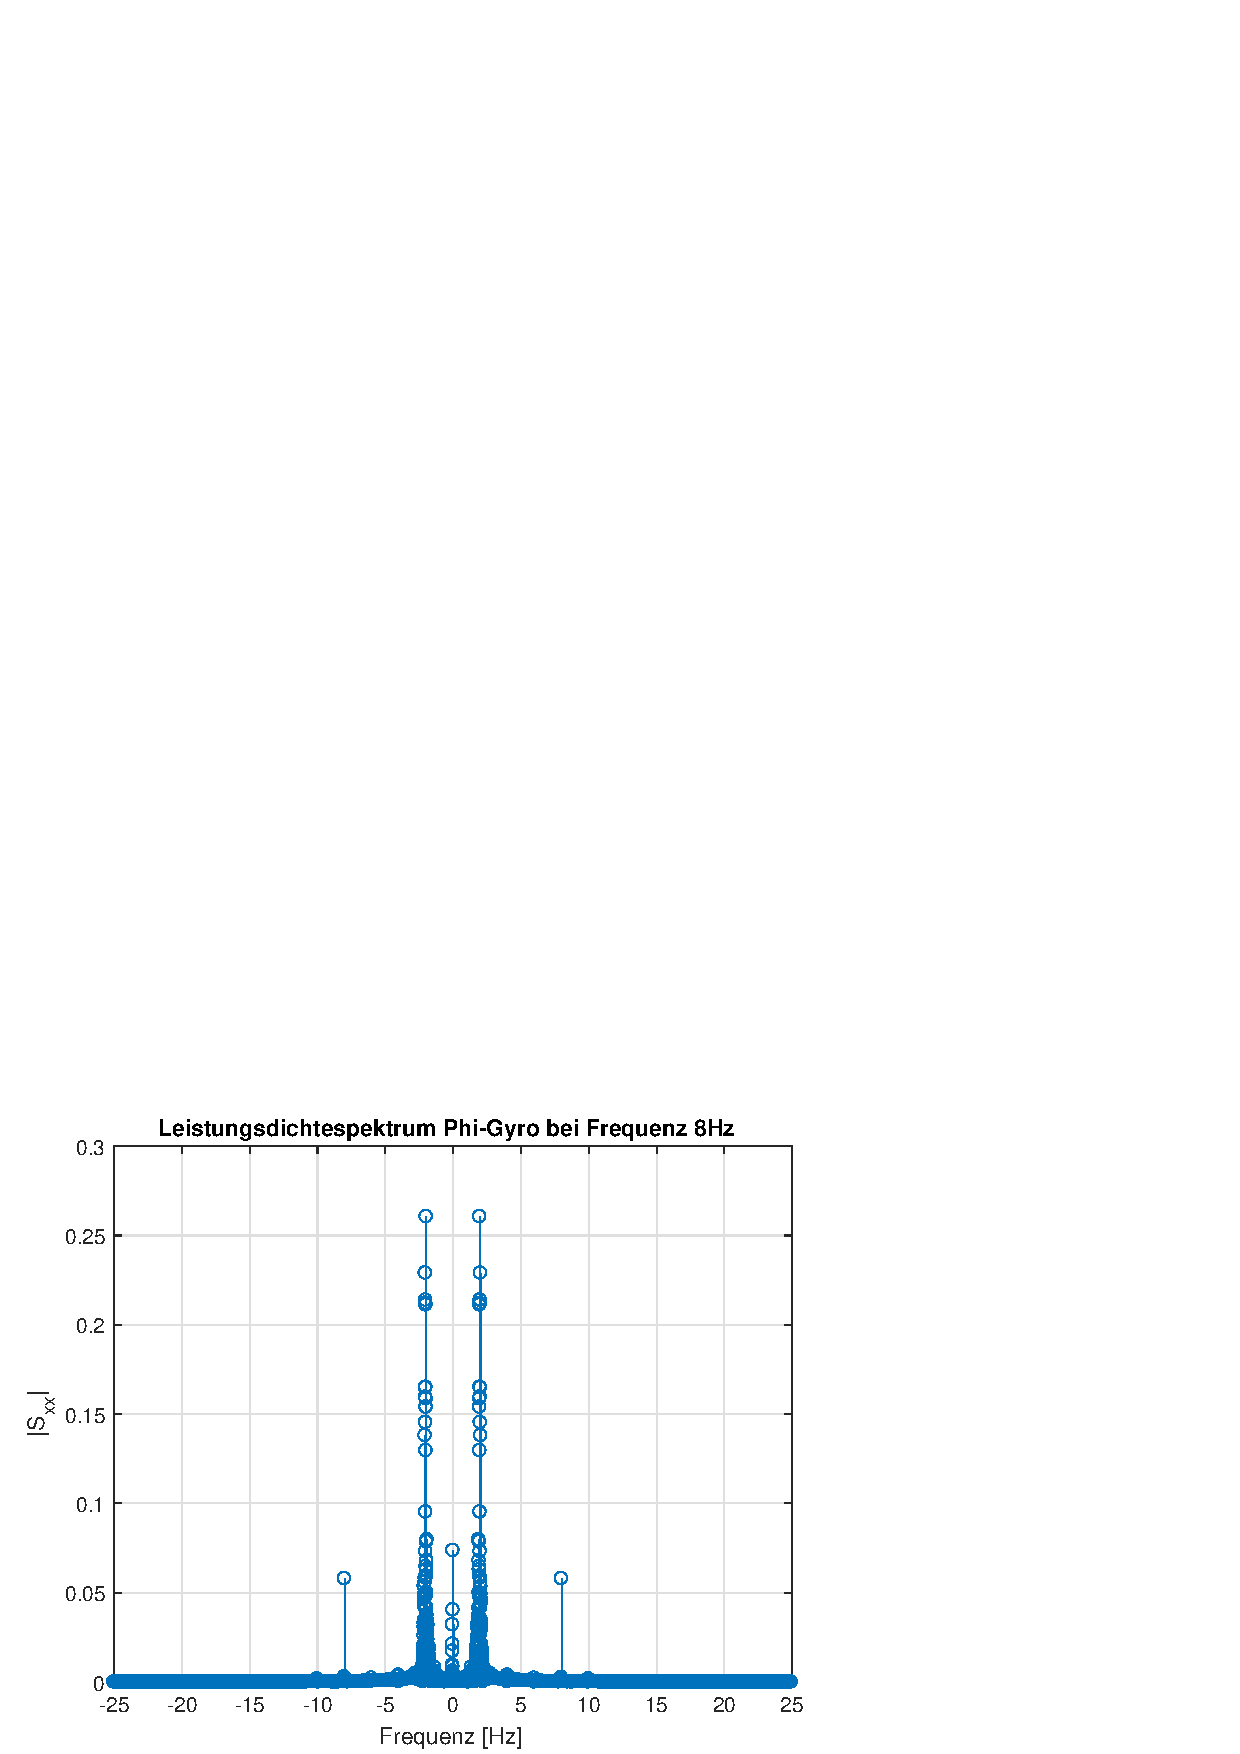
\includegraphics[width=0.5\linewidth]{img/lds_phi_g_9}
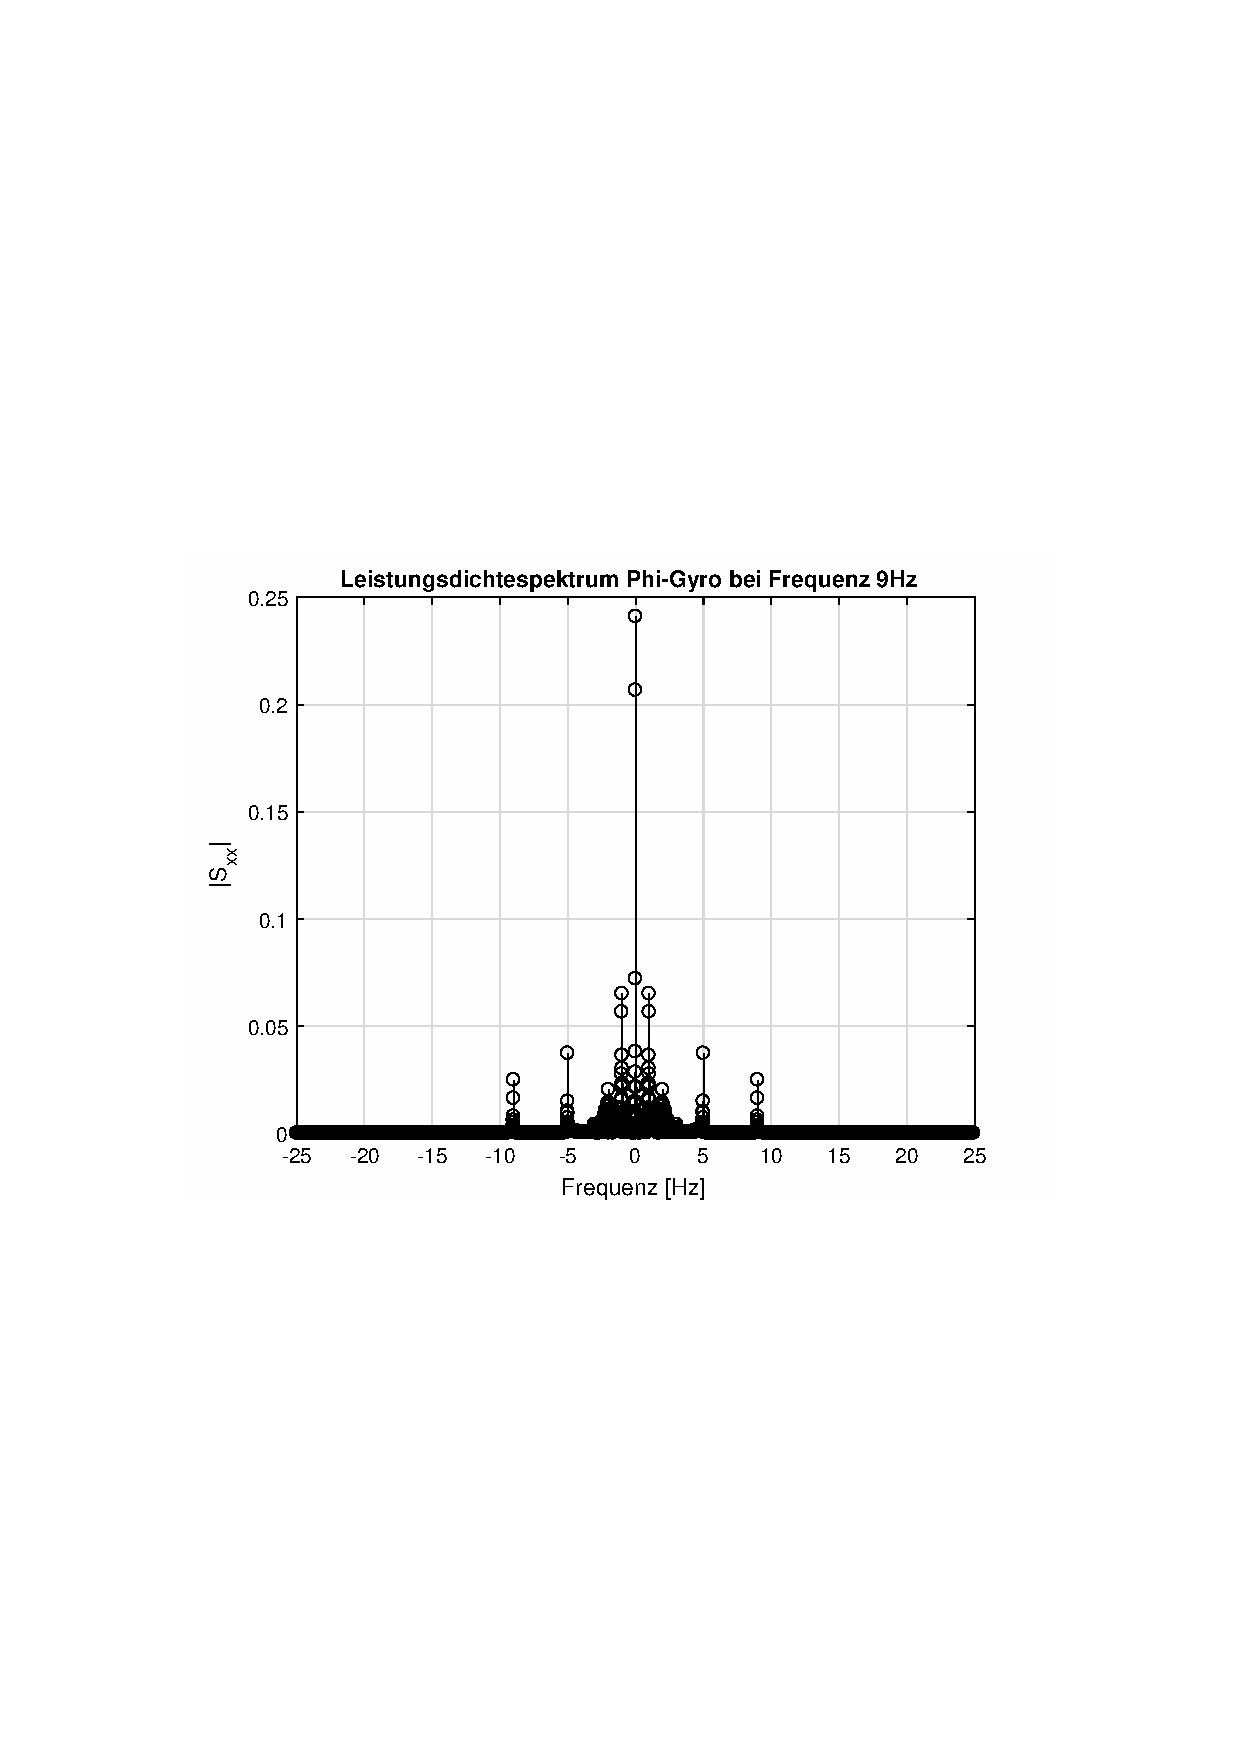
\includegraphics[width=0.5\linewidth]{img/lds_phi_g_10}
\end{figure}
\begin{figure}[h!]
\centering
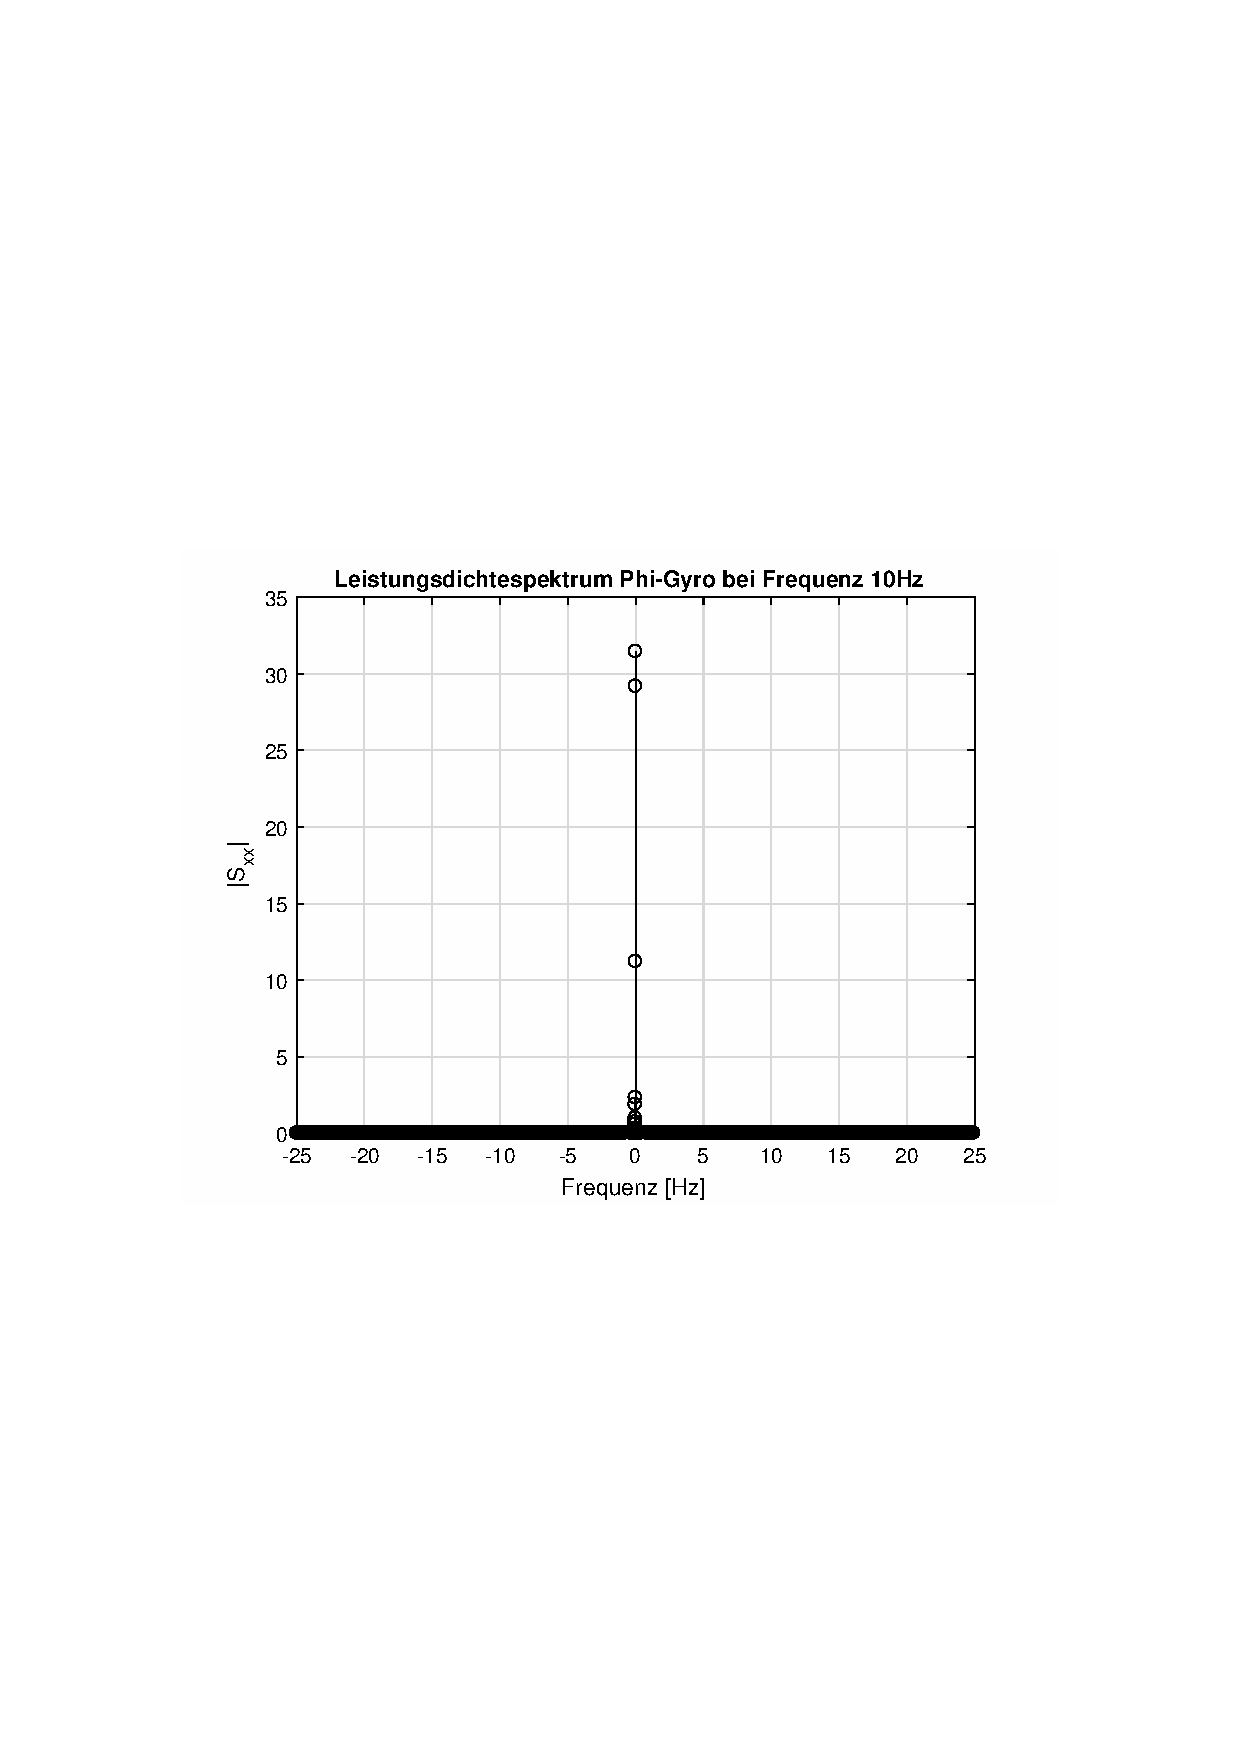
\includegraphics[width=0.5\linewidth]{img/lds_phi_g_11}
\end{figure}
\end{document}